\chapter{Search for di-Higgs Production in the Channel} % todo: yybb not capitalized?

\section{Analysis Overview}

Previous results were presented with an integrated luminosity of 36.1 fb$^{-1}$ representing ATLAS dataset in 2015 and 2016 \cite{HIGG-2016-15}, and were consistent with Standard Model expectations. The non-resonant analysis set an observed (expected) 95\% CL upper limit on the $HH$ cross-section of 0.73 (0.93) pb, corresponding to 22 (28) times the SM prediction. This Higgs trilinear coupling is constrained between $-8.2 < \kappa_\lambda < 13.2$ at 95\% CL ($-8.3 < \kappa_\lambda < 13.2$ expected). The resonant analysis presented within the context of a narrow width scalar coupling to the di-Higgs system as a function of $m_X$. The observed (expected) limits are between 1.1 pb (0.9 pb) and 0.12 pb (0.15 pb) over the range of $\unit{260}{\GeV} < m_X < \unit{1000}{\GeV}$.

\section{Data and Simulated Samples}


\subsection{Data}

The analysis presented uses $pp$ collision data recorded by the ATLAS experiment at the LHC in 2015 and 2016, the first half of ``Run 2.'' After detector and data quality requirements, the total collected data corresponds to 36.1 \ifb. The loose diphoton trigger is used for this search, \texttt{HLT\_g35\_loose\_g25\_loose}, which triggers on diphoton events where the leading (subleading) photon \pt is greater than 35\% (25\%) the diphoton invariant mass.

\subsection{Simulated Samples}

Simulation is generated as outlined in Chapter \ref{ch:eventreco} in order to compare prediction to data. Independent samples are made for the considered signal hypotheses, as well as for the predominant backgrounds.

\subsubsection{Signal Samples}

This analysis considers two signals sources: \gls{SM} non-resonant di-Higgs production and resonant di-Higgs production through a scalar resonance.

\noindent\textbf{Non-resonant \gls{SM} Signal Samples}\\
\indent The non-resonant di-Higgs signal sample corresponding to \gls{SM} \gls{ggF} \hh production is generated at \gls{NLO} in \gls{QCD} through an \gls{EFT}.

\noindent\textbf{Non-resonant Varied \klambda Signal Samples}\\
\indent Samples for non-resonant di-Higgs production with varied \klambda were generated at values $\klambda = 0, \pm 1, \pm 2, \pm 4, \pm 6, \pm 10$. These samples were generated at \gls{LO}, then reweighted to \gls{NNLO} through a $K$-factor, taking the ratio of the cross-sections of the FT\textsubscript{approx} \gls{SM} non-resonant signal sample (at \gls{NNLO}) and the $\klambda =1$ sample (at \gls{LO}).

For generic \klambda, an interpolation function can be used to predict the amplitude, and thus the signal yield. The amplitude can be written as

\begin{equation}
  A(k_t,\klambda) = k_t^2 B + k_t \klambda T
\end{equation}

Where $B$ is the contribution from the box diagram (with two $th$ vertices, thus squared), $T$ is the contribution from the trilinear diagram (containing one $th$ and one $hhh$ vertex). If we square this amplitude and vary \klambda (consider values 0, 1, and 10),

\begin{align}
  &|A(k_t,\klambda)|^2 = k_t^4 |B|^2 + k_t^2\klambda^2 |T|^2 + k_t^3\klambda(B^*T + BT^*)\\
  &|A(1,0)|^2 = |B|^2\\
  &|A(1,1)|^2 = |B|^2 + |T|^2 + (B^*T + BT^*)\\
  &|A(1,10)|^2 = |B|^2 + 100|T|^2 + 10(B^*T + BT^*)
\end{align}

We can then combine these equations to express the squared amplitude in terms of the amplitudes of the varied reference samples
\begin{equation}
  |A(k_t,\klambda)|^2 = k_t^2 \left[ 
    \frac{90 k_t^2 + 9\klambda^2 - 99k_t\klambda}{90}|A(1,0)|^2 +
    \frac{100 k_t\klambda - 10\klambda^2}{90}|A(1,1)|^2 +
    \frac{\klambda^2 - k_t\klambda}{90}|A(1,1)|^2 \right]
\end{equation}
% todo : add to appendix validation plots?

\subsubsection{Background Samples}

The dominant background in this analysis are the non-resonant \myy continuum events. Additionally, mono-Higgs boson production is a subdominant background to this analysis. 

\noindent\textbf{\yy-Continuum}\\
\indent The \yy-continuum sample is generated using \SHERPA, generating processes including two photons and jets (\yy+jets). This \gls{MC} sample is used predominantly for shape information, since normalization is taken through a data-driven approach. 

\noindent\textbf{Mono-Higgs Production}\\
\indent The following mono-Higgs production channels are considered: gluon-gluon fusion ($ggH$), vector-boson fusion ($VBF\ H$) Z-associated production ($ZH$), W-associated production ($WH$), single and top quark pair associated production ($tH$ and \tth, respectively), and bottom quark pair associated production ($b\bar{b}H$). Rates for these samples are taken from the 2016 Yellow Report \cite{yellow-report}. The generators for these samples vary, and are listed in Table \ref{tab:single-higgs-samples}, along with the cross-section times \gls{BR} for each sample.

\begin{table}[htbp]
  \begin{center}
    \caption[Mono-Higgs boson backgrounds considered, including generator and PDF used to produce each sample]{Mono-Higgs boson backgrounds considered, including generator and PDF used to produce each sample. Cross-section for each sample is shown, multiplied by the $H\rightarrow \gamma\gamma$ \gls{BR} of 0.00227. Cross-sections assume $\sqrt{s}=\unit{13}{\TeV}$ and $m_{H}=\unit{125}{\GeV}$.}
    \label{tab:single-higgs-samples}
    \begin{tabular}{|c|c|c|}
      \hline
      Process & Generator+PDF & $\sigma \times \mathcal{B}\ (H\rightarrow\gamma\gamma)$ \\
      \hline
      $ggH$ & \makecell{\POWHEG+ \peight \\ PDF4LHC15}& 0.1101404\\
      \hline
      $VBF\ H$ & \makecell{\POWHEG+ \peight \\ PDF4LHC15}& 0.00857833\\
      \hline
      $W^-H$ & \makecell{\POWHEG+ \peight \\ PDF4LHC15}& 0.00120605\\
      \hline
      $W^+H$ & \makecell{\POWHEG+ \peight \\ PDF4LHC15}& 0.00190226\\
      \hline
      $ZH$ & \makecell{\POWHEG+ \peight \\ PDF4LHC15}& 0.001724519\\
      \hline
      $ggZH$ & \makecell{\POWHEG+ \peight \\ PDF4LHC15}& 0.000278529\\
      \hline
      \tth & \makecell{\peight \\ A14 NNPDF23LO}& 0.001149755\\
      \hline
      $b\bar{b}H$ (positive) & \makecell{\AMCatNLO+ \peight \\ A14 NNPDF23LO}& 0.00110390\\
      \hline
      $b\bar{b}H$ (negative) & \makecell{\AMCatNLO+ \peight \\ A14 NNPDF23LO}& -8.95378e-05\\
      \hline
      $tH$ ($t$-channel) & \makecell{\MADGRAPH+ \peight \\ A14 CT10ME}& 0.00016857\\
      \hline
      $tH$ ($W$-associated) & \makecell{\AMCatNLO+ \peight \\ UEEE5 CTEQ6L1 CT10ME}& 3.44359e-05\\
      \hline
    \end{tabular}
  \end{center}
\end{table}


\section{Object Definition}
\subsection{Photons}

Selected photons for this analysis are converted or unconverted photons which pass tight ID cuts (outlined in Section \ref{ssec:em-signatures}). Photons must have $\pt > \unit{25}{\GeV}$ and $\abseta < 2.37$. Additionally, the crack region of $1.37 < \abseta < 1.52$ is rejected.

Photons must pass an ambiguity tool is used to differentiate overlapping photons and electrons \cite{r1-photonID}.
%TODO : continue this (p28)

The leading photon \pt distribution is shown in Figure \ref{fig:photon_l_pt}, the subleading is shown in Figure \ref{fig:photon_s_pt}.

\begin{figure}[htbp]
  \centering
  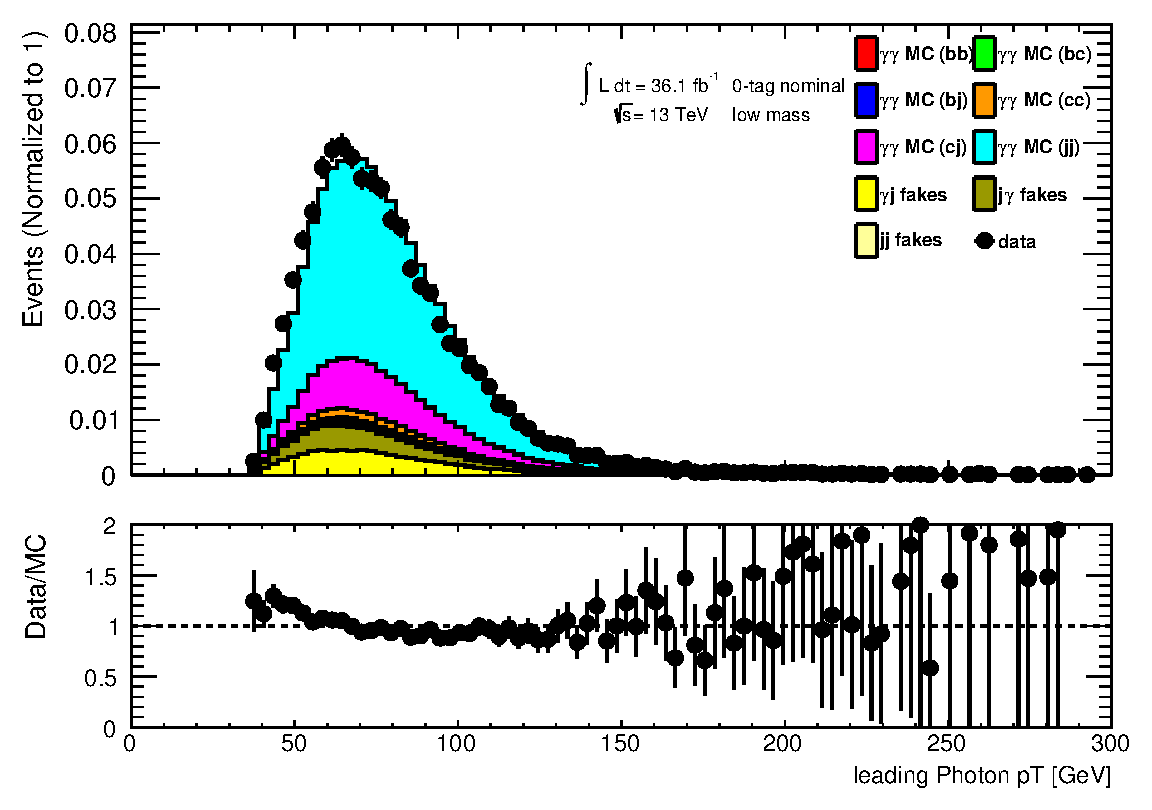
\includegraphics[width=0.48\textwidth]{chapters/chapter5_yybb/images/data_MC_comparison/h_CR_l_0t_nominal_leadingPhoton_pt.pdf}
  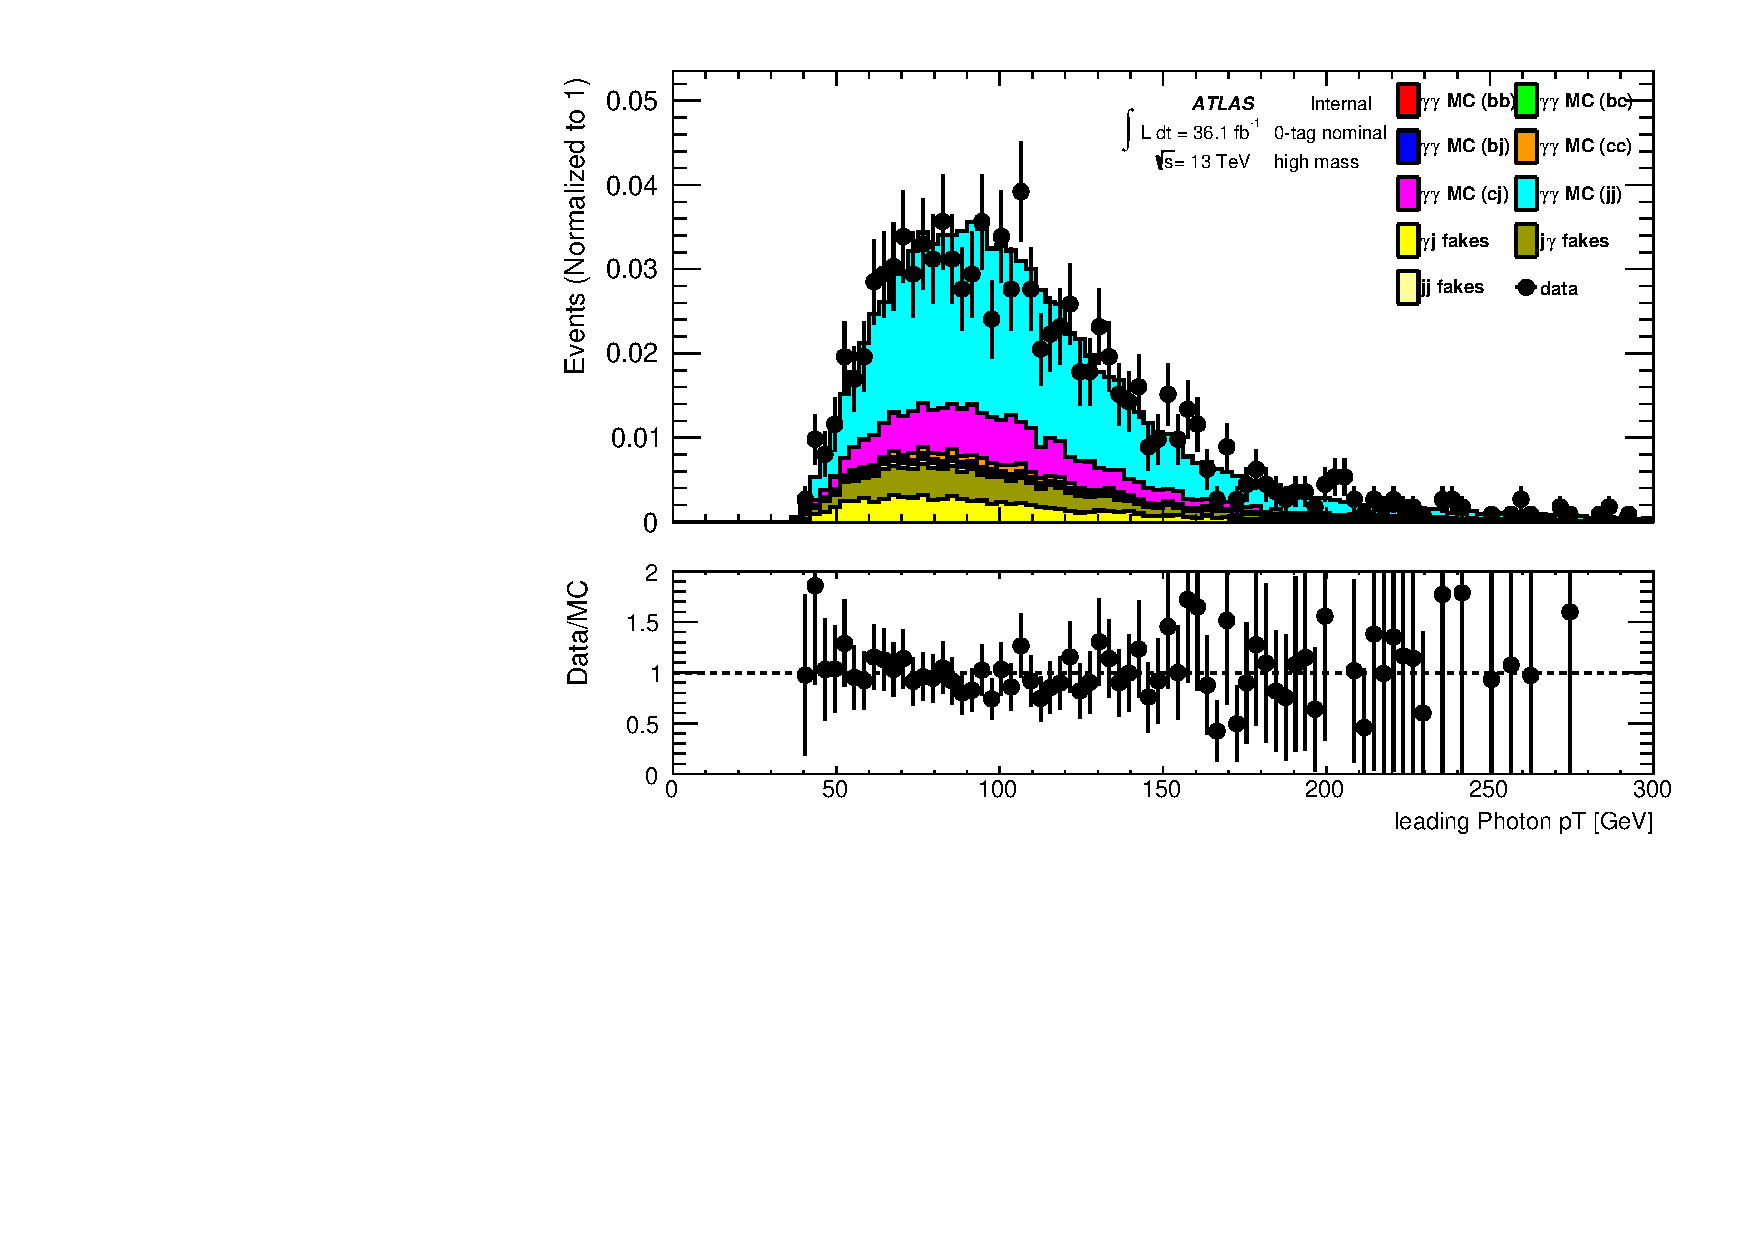
\includegraphics[width=0.48\textwidth]{chapters/chapter5_yybb/images/data_MC_comparison/h_CR_h_0t_nominal_leadingPhoton_pt.pdf}
  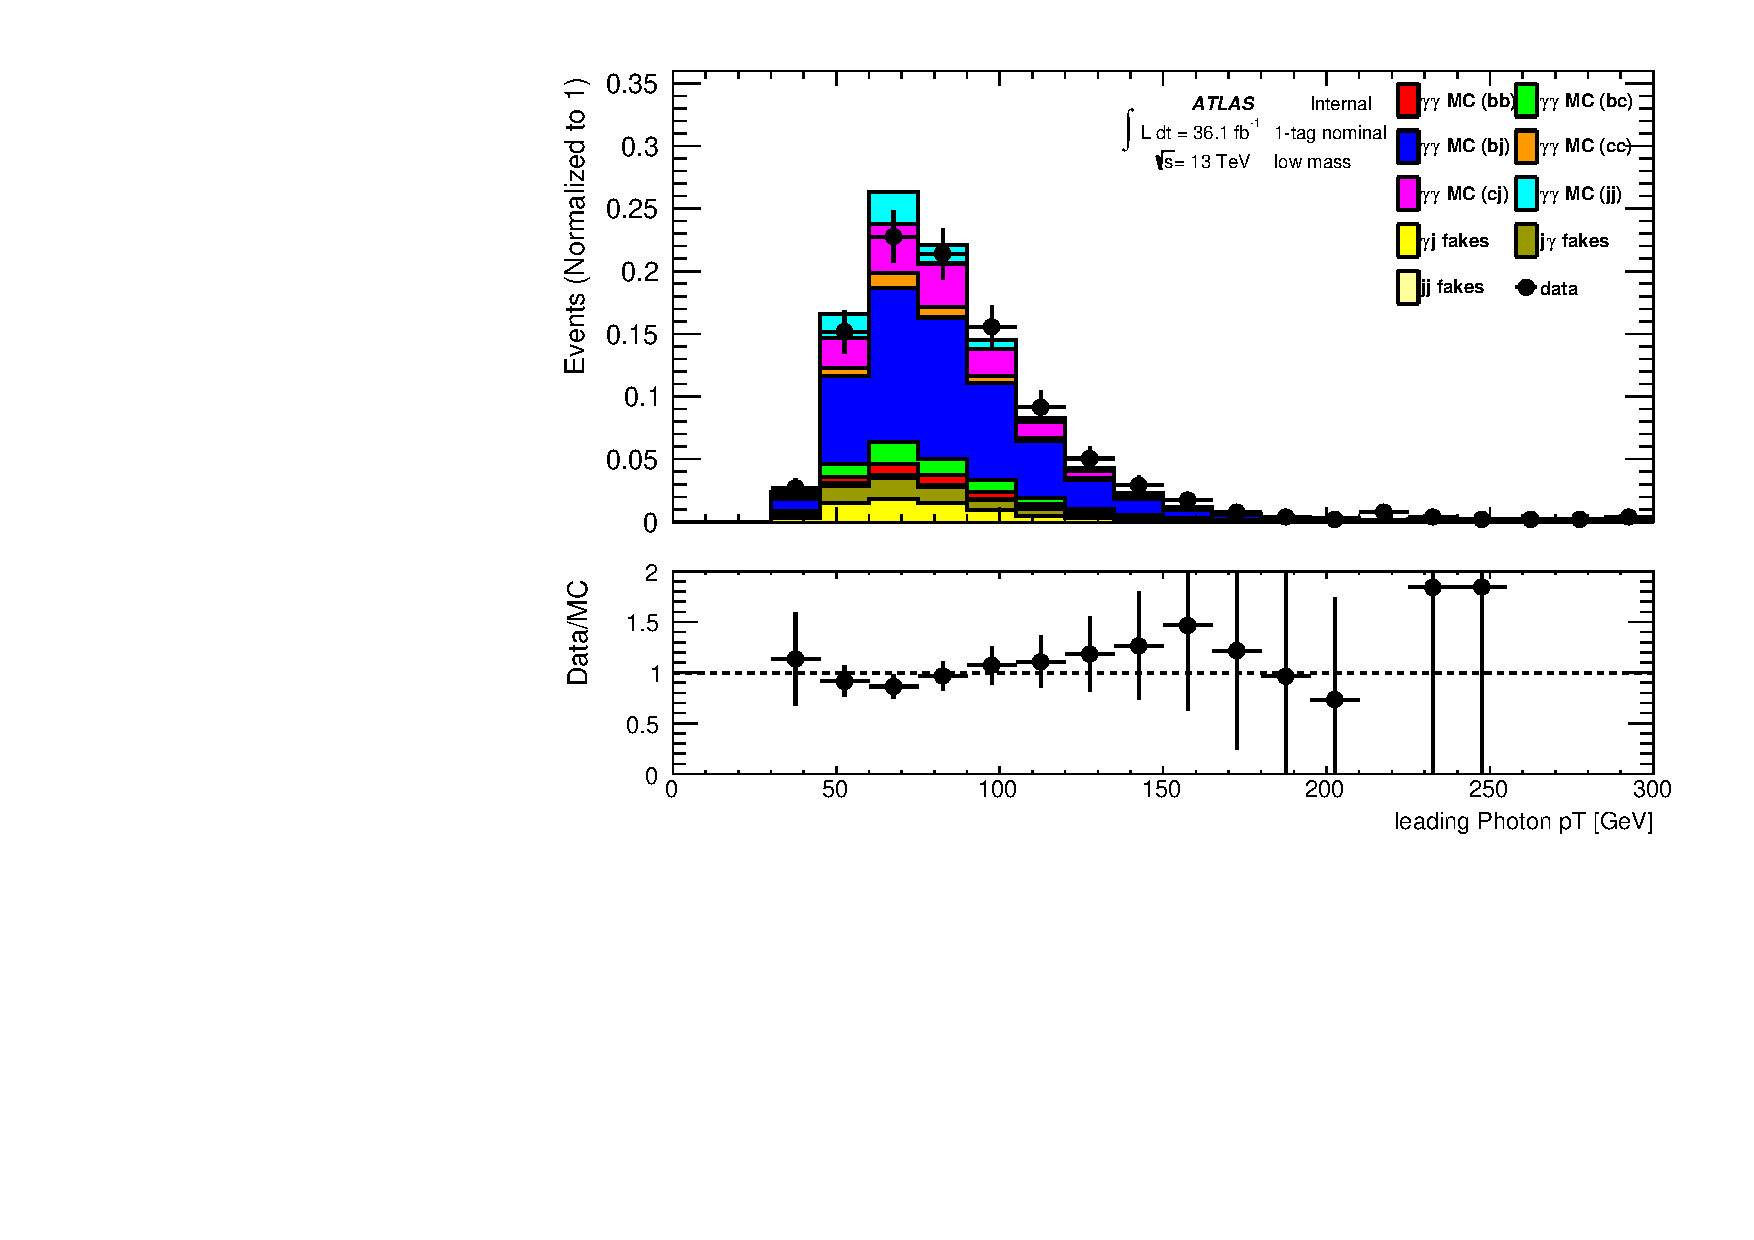
\includegraphics[width=0.48\textwidth]{chapters/chapter5_yybb/images/data_MC_comparison/h_SR_l_1t_nominal_leadingPhoton_pt.pdf}
  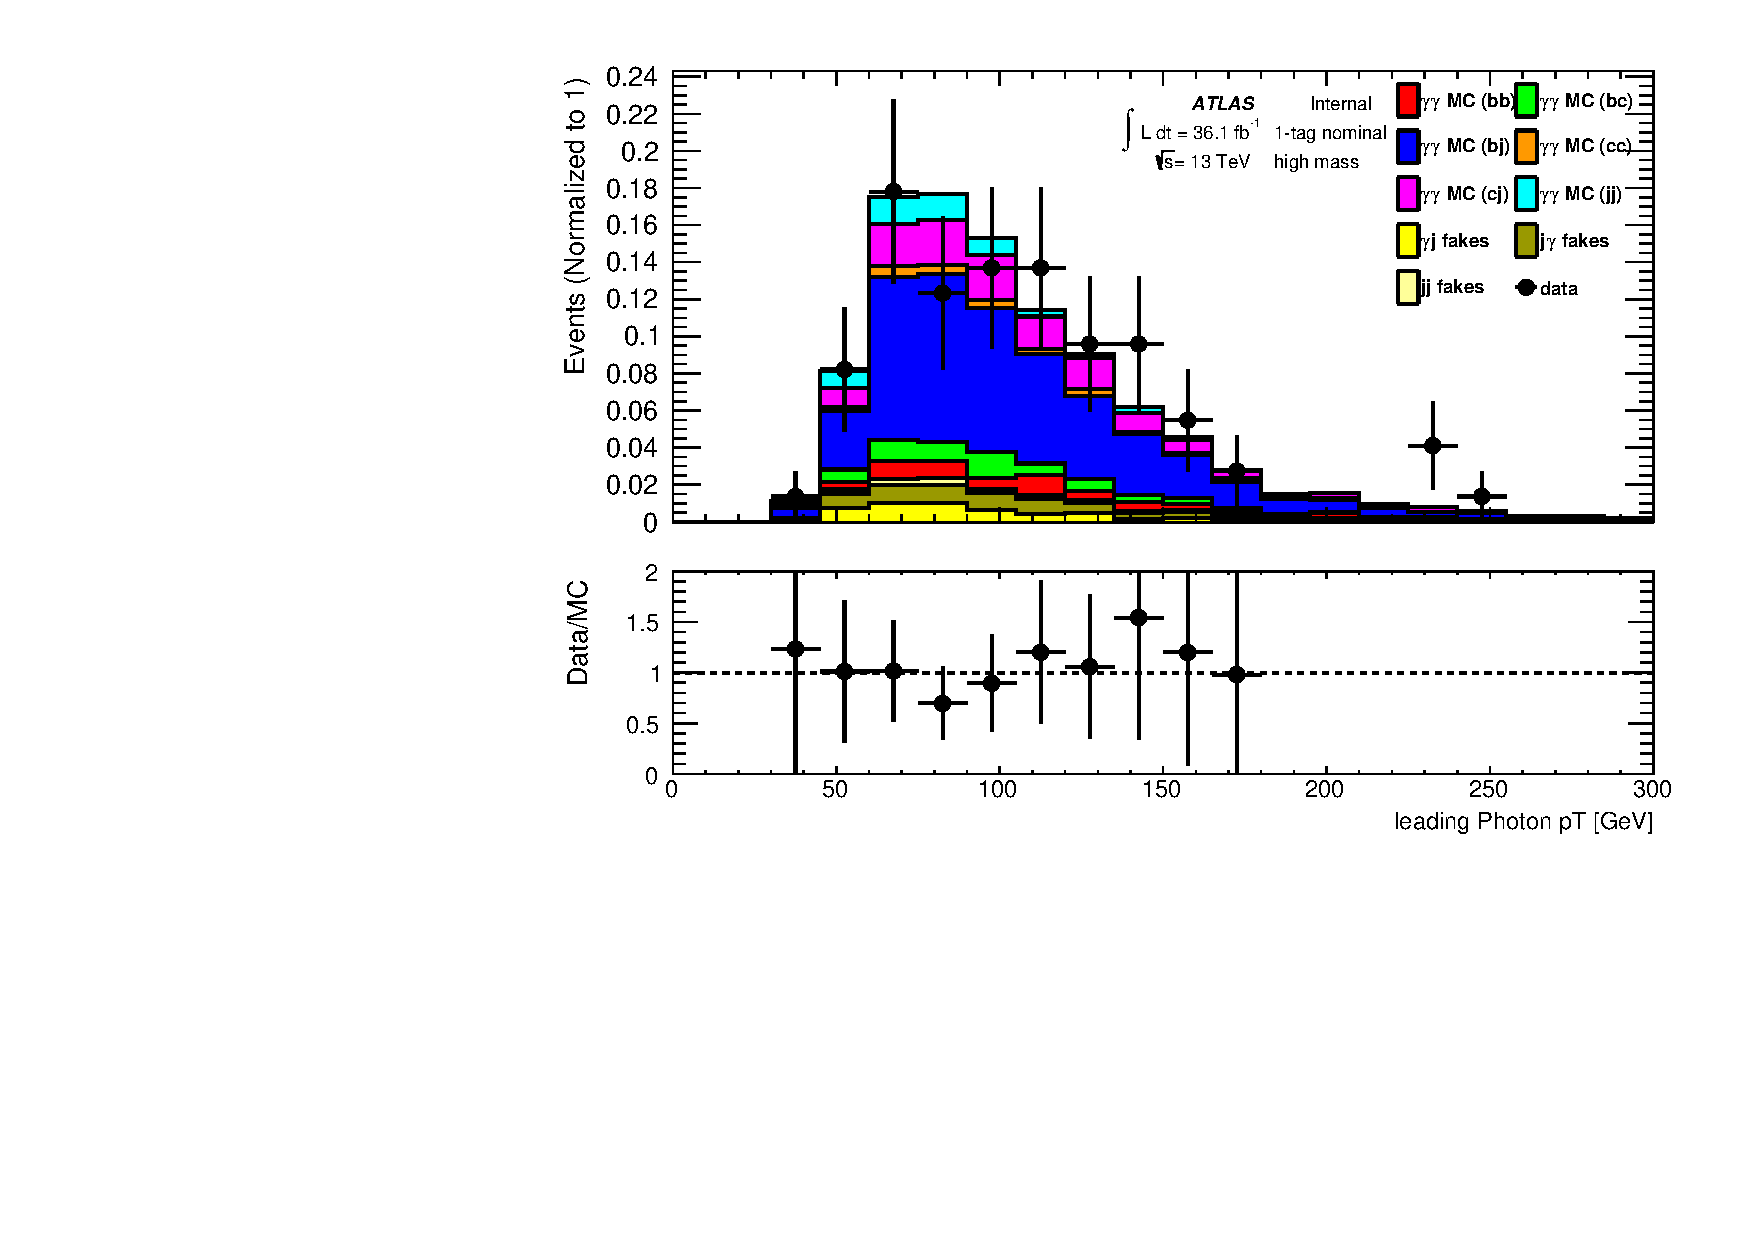
\includegraphics[width=0.48\textwidth]{chapters/chapter5_yybb/images/data_MC_comparison/h_SR_h_1t_nominal_leadingPhoton_pt.pdf}
  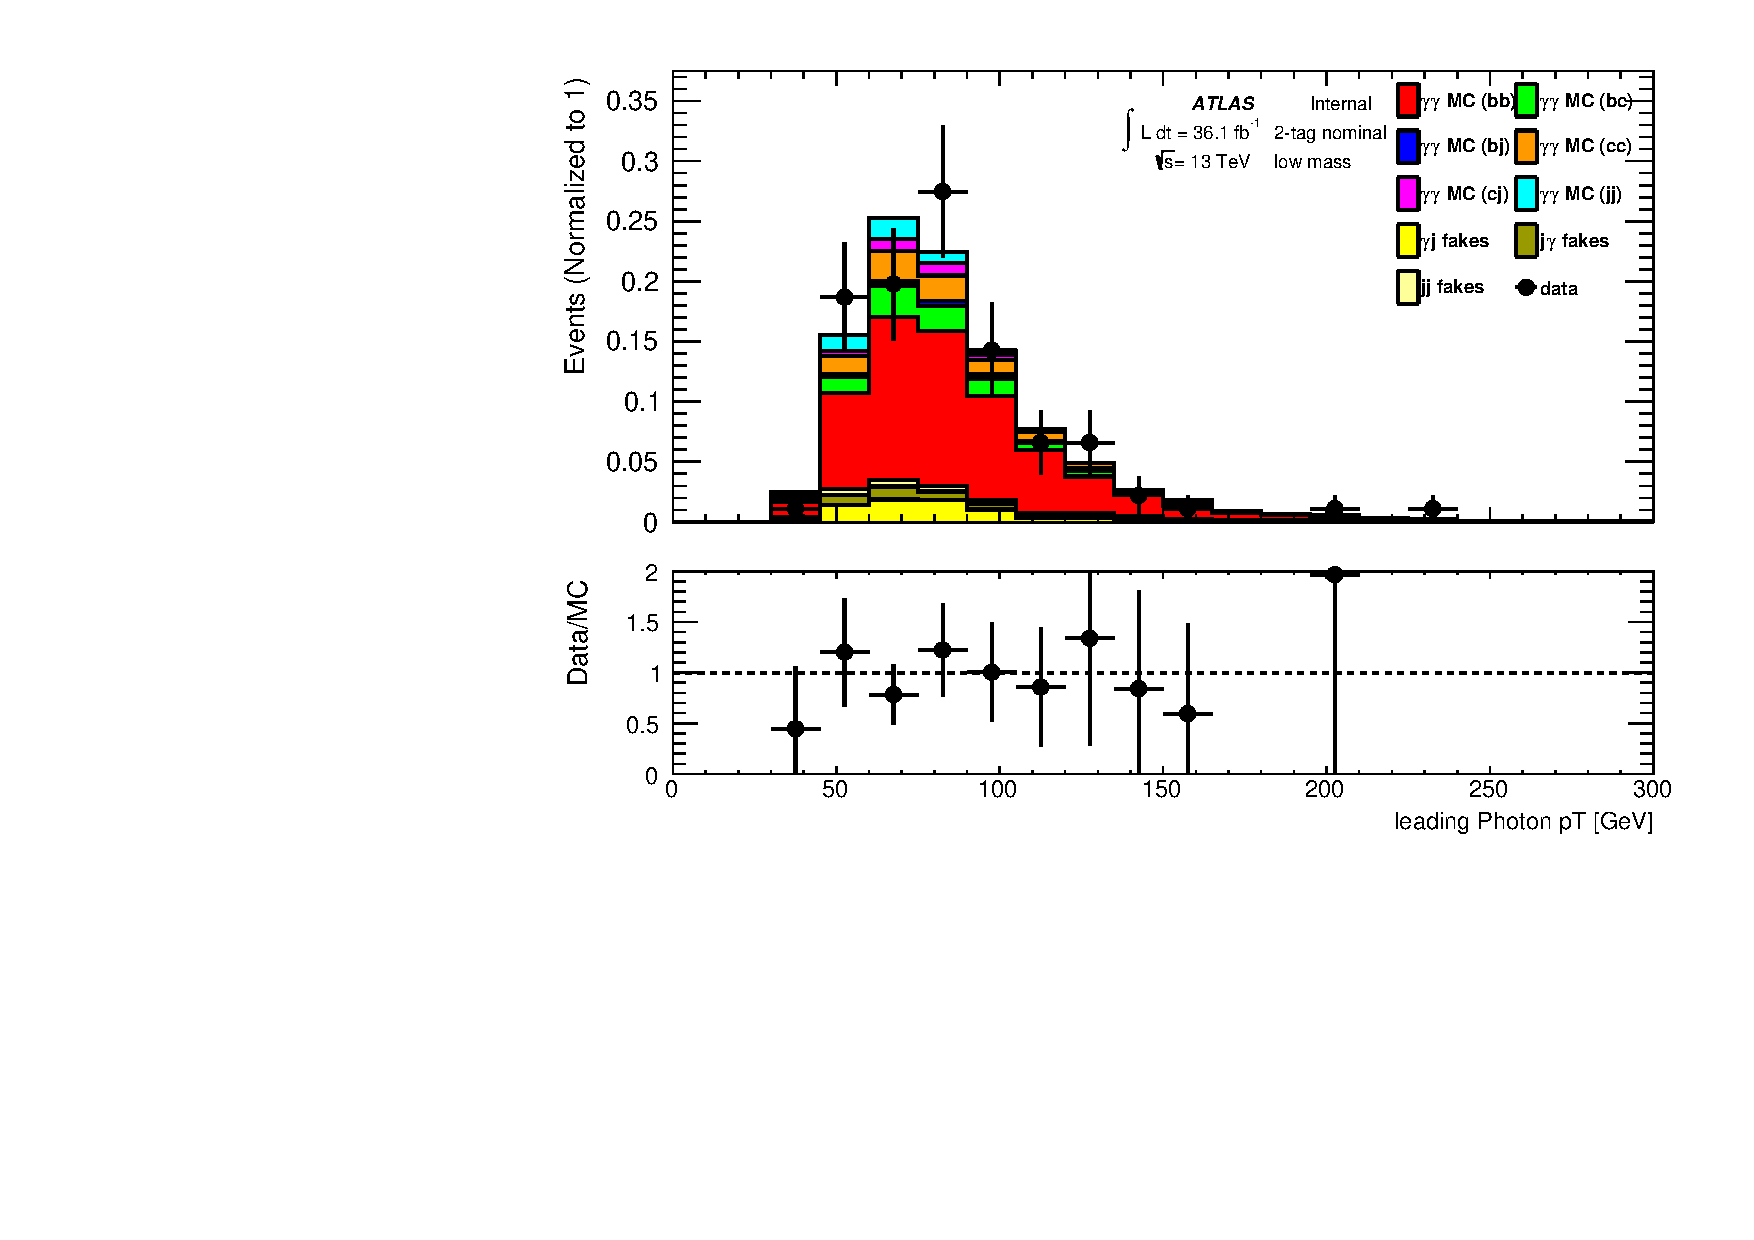
\includegraphics[width=0.48\textwidth]{chapters/chapter5_yybb/images/data_MC_comparison/h_SR_l_2t_nominal_leadingPhoton_pt.pdf}
  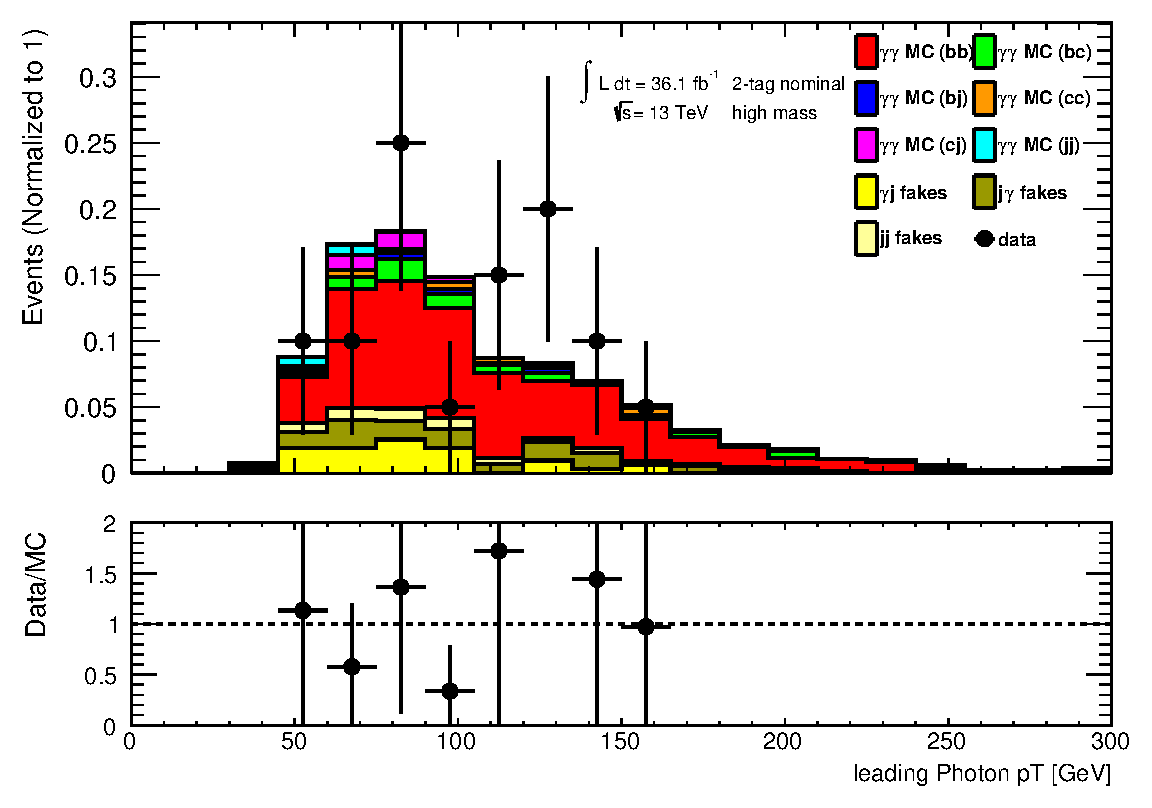
\includegraphics[width=0.48\textwidth]{chapters/chapter5_yybb/images/data_MC_comparison/h_SR_h_2t_nominal_leadingPhoton_pt.pdf}
  \caption[Leading photon \pt.]{Leading photon \pt by b-tagging category. The low (left) and high (right) mass selections are shown. Both data and MC are normalized such that the integral is 1.
  \label{fig:photon_l_pt}}
\end{figure}

\begin{figure}[htbp]
  \centering
  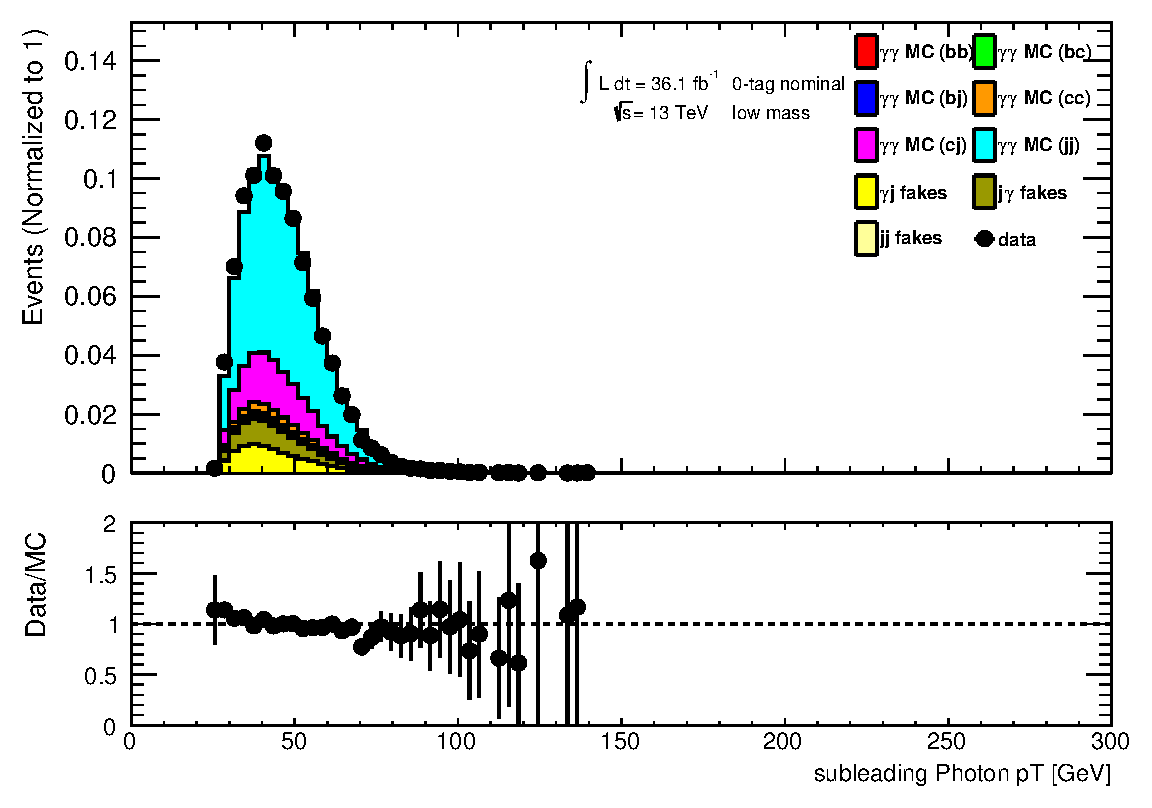
\includegraphics[width=0.48\textwidth]{chapters/chapter5_yybb/images/data_MC_comparison/h_CR_l_0t_nominal_subleadingPhoton_pt.pdf}
  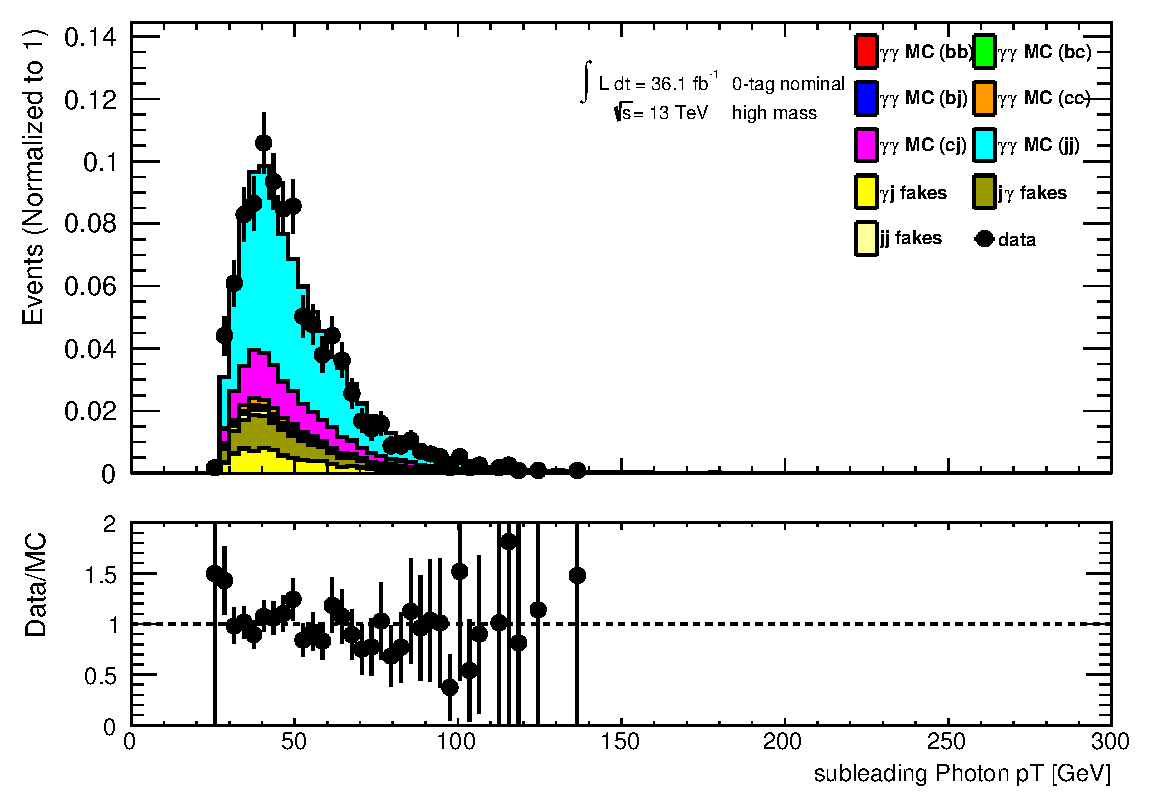
\includegraphics[width=0.48\textwidth]{chapters/chapter5_yybb/images/data_MC_comparison/h_CR_h_0t_nominal_subleadingPhoton_pt.pdf}
  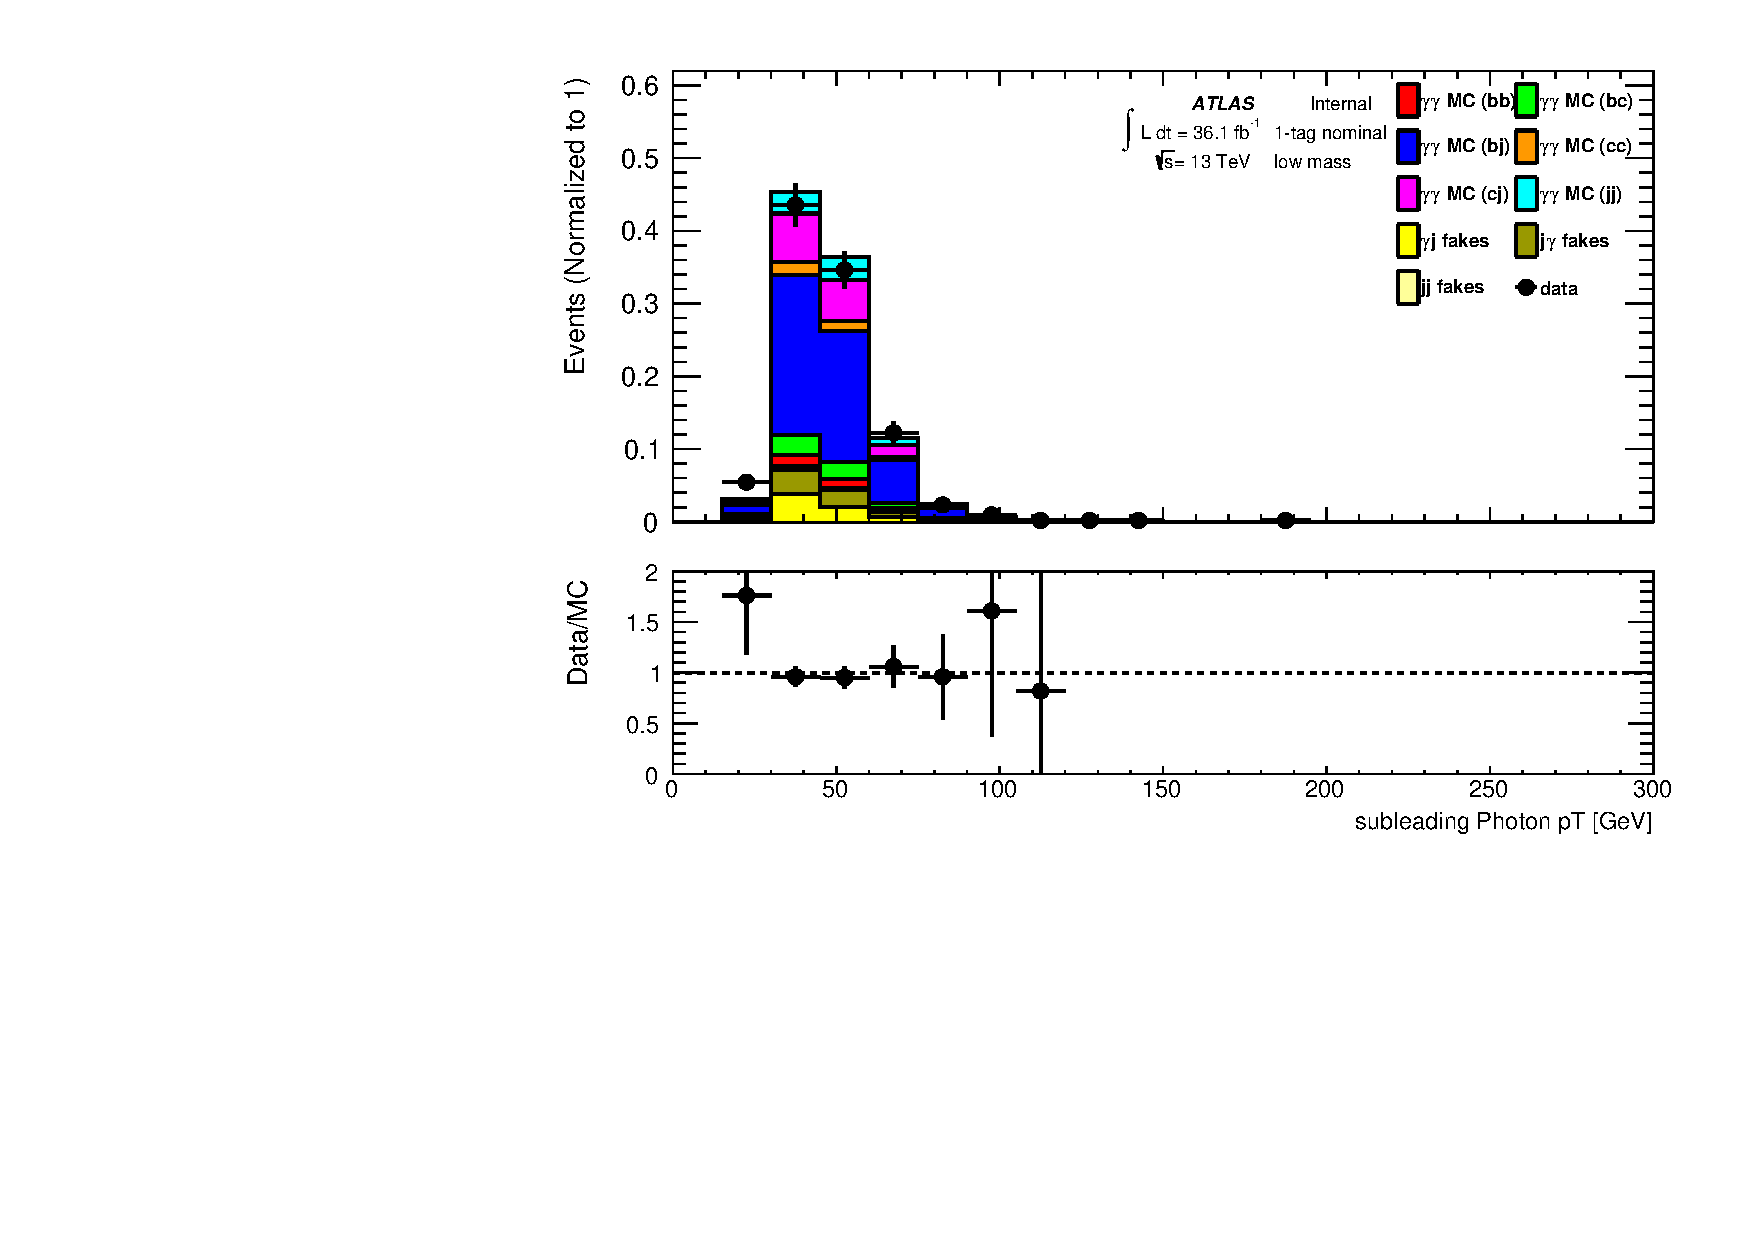
\includegraphics[width=0.48\textwidth]{chapters/chapter5_yybb/images/data_MC_comparison/h_SR_l_1t_nominal_subleadingPhoton_pt.pdf}
  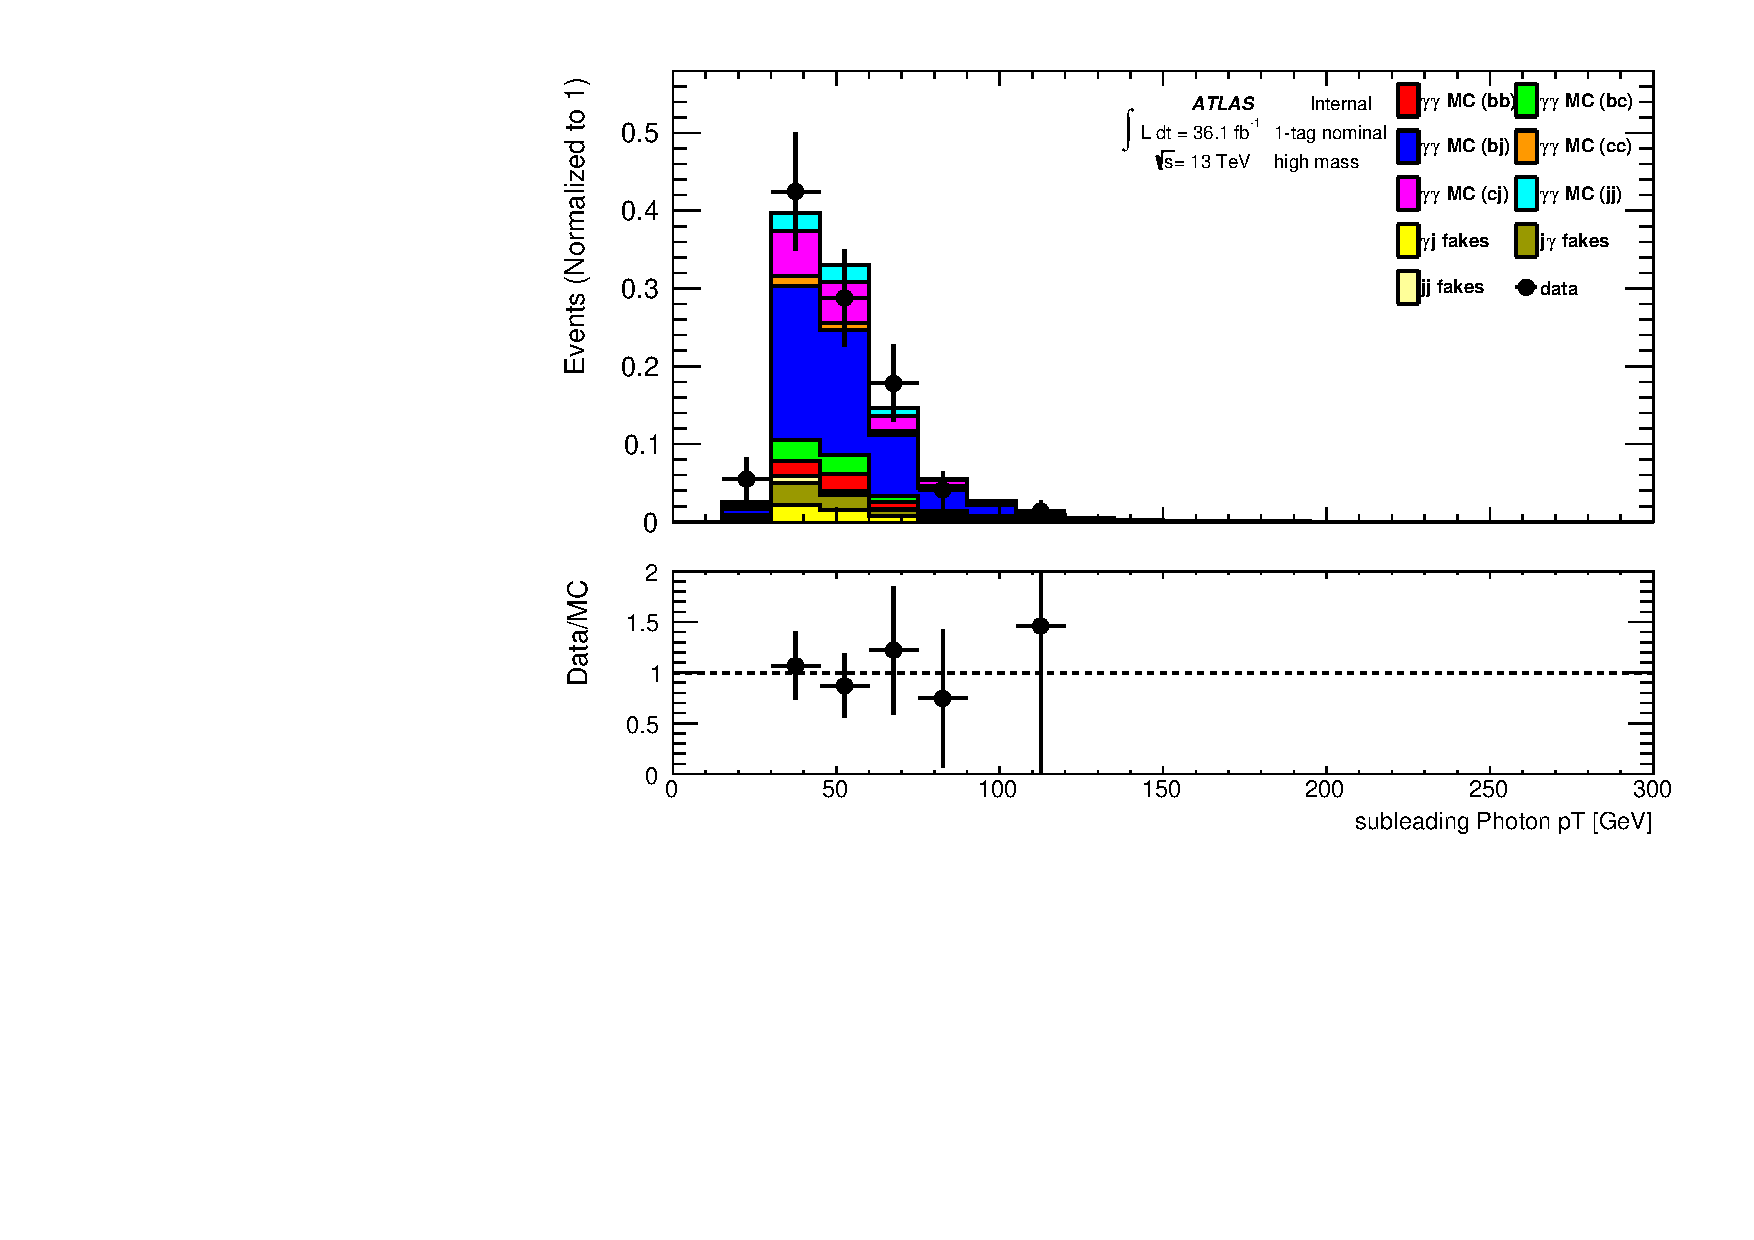
\includegraphics[width=0.48\textwidth]{chapters/chapter5_yybb/images/data_MC_comparison/h_SR_h_1t_nominal_subleadingPhoton_pt.pdf}
  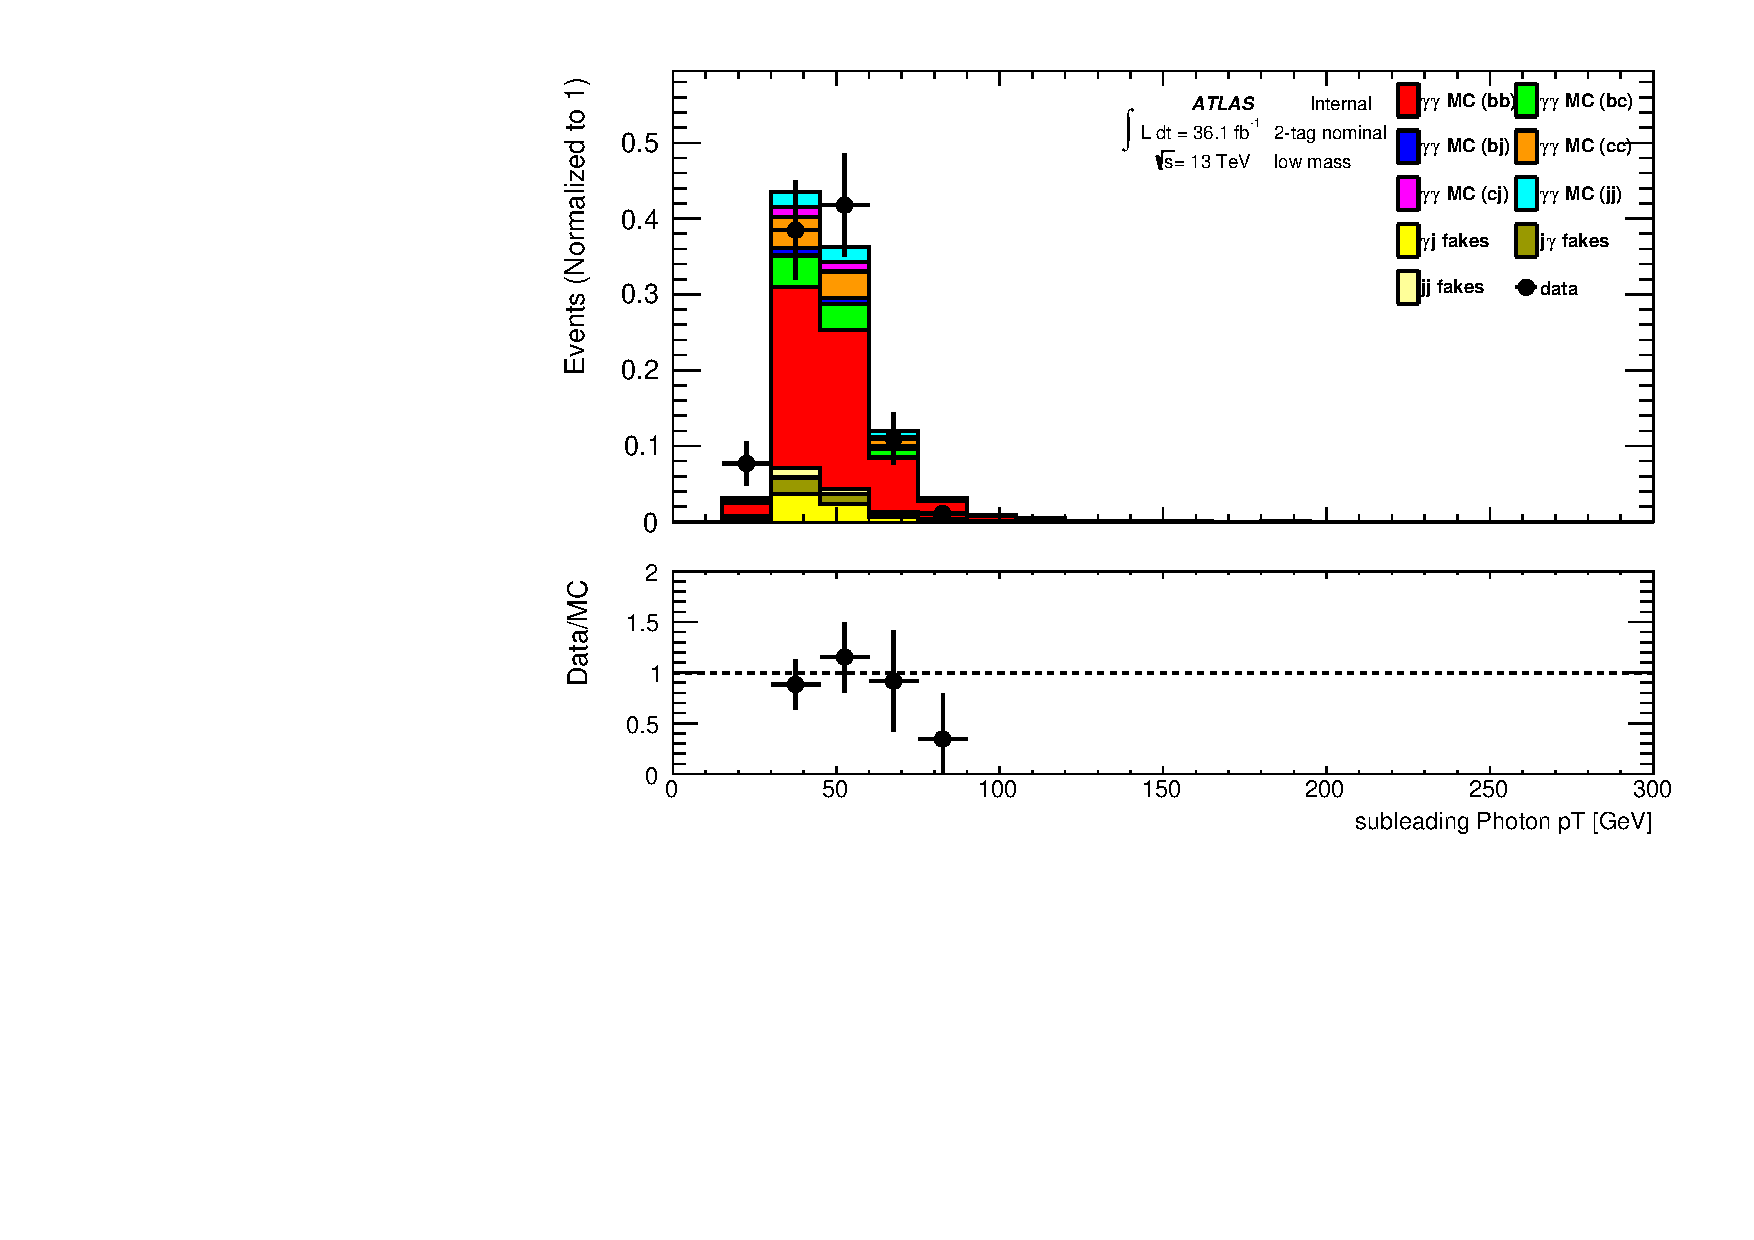
\includegraphics[width=0.48\textwidth]{chapters/chapter5_yybb/images/data_MC_comparison/h_SR_l_2t_nominal_subleadingPhoton_pt.pdf}
  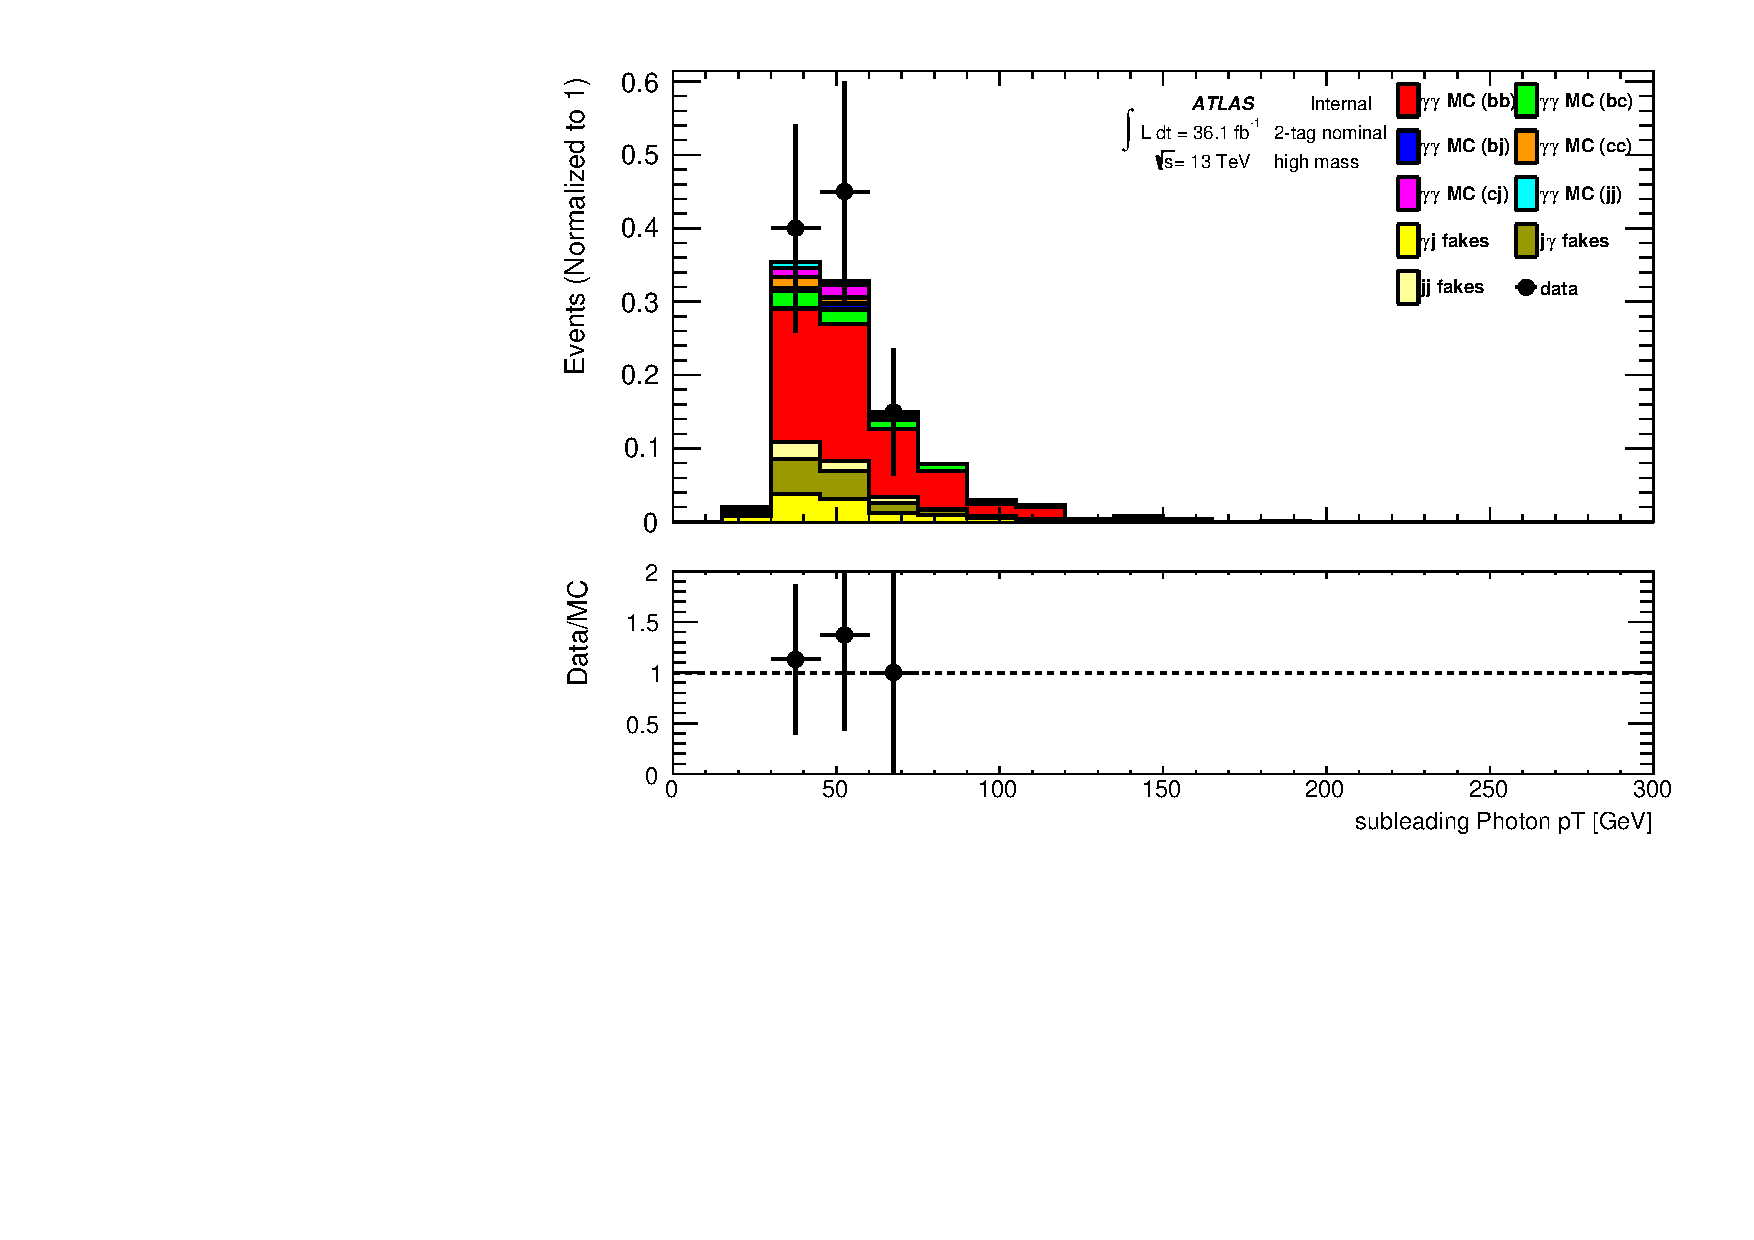
\includegraphics[width=0.48\textwidth]{chapters/chapter5_yybb/images/data_MC_comparison/h_SR_h_2t_nominal_subleadingPhoton_pt.pdf}
  \caption[Subleading photon \pt.]{Subleading photon \pt by b-tagging category. The low (left) and high (right) mass selections are shown. Both data and MC are normalized such that the integral is 1.
  \label{fig:photon_s_pt}}
\end{figure}


\subsection{Jets}

Jets are defined using the \antikt algorithm with $R=0.4$, using jets with energy corrected for pile-up effects and direction readjusted to the primary vertex (EM-JES jets). Jets considered must have $\pt > \unit{25}{\GeV}$ and be within the tagging region, $\abseta < 2.5$. The following additional requirements are applied\footnote{This selection is similar to that of the default jet selection for ATLAS $H\rightarrow \yy$ analyses. The $\abseta < 2.5$ is an additional requirement imposed atop that selection for b-tagging.}:

\begin{itemize}
  \item Jets with $\pt < \unit{50}{\GeV}$ and $\abseta < 2.4$ must pass the ``default'' \gls{JVT} requirement, with $|\text{JVT}| \geq 0.59$ \cite{JVT}.
  \item Events that contain a jet passing the ``LooseBad'' cut are vetoed. 
  \item Jets with $\Dr < 0.4$ from a tight, isolated photon are vetoed.
  \item Jets with $\Dr < 0.2$ from a selected electron are vetoed.
\end{itemize}



Following this selection, candidate jets are selected in the following way:
\begin{itemize}
  \item In the 0-tag control region, the two leading jets are the candidate jets.
  \item In the 1-tag region, one of the jets is the b-tagged jet, the other is selected via a \gls{BDT}
  \item In the 2-tag region, the two b-tagged jets are the candidate jets.
\end{itemize}

\begin{figure}[htbp]
  \centering
  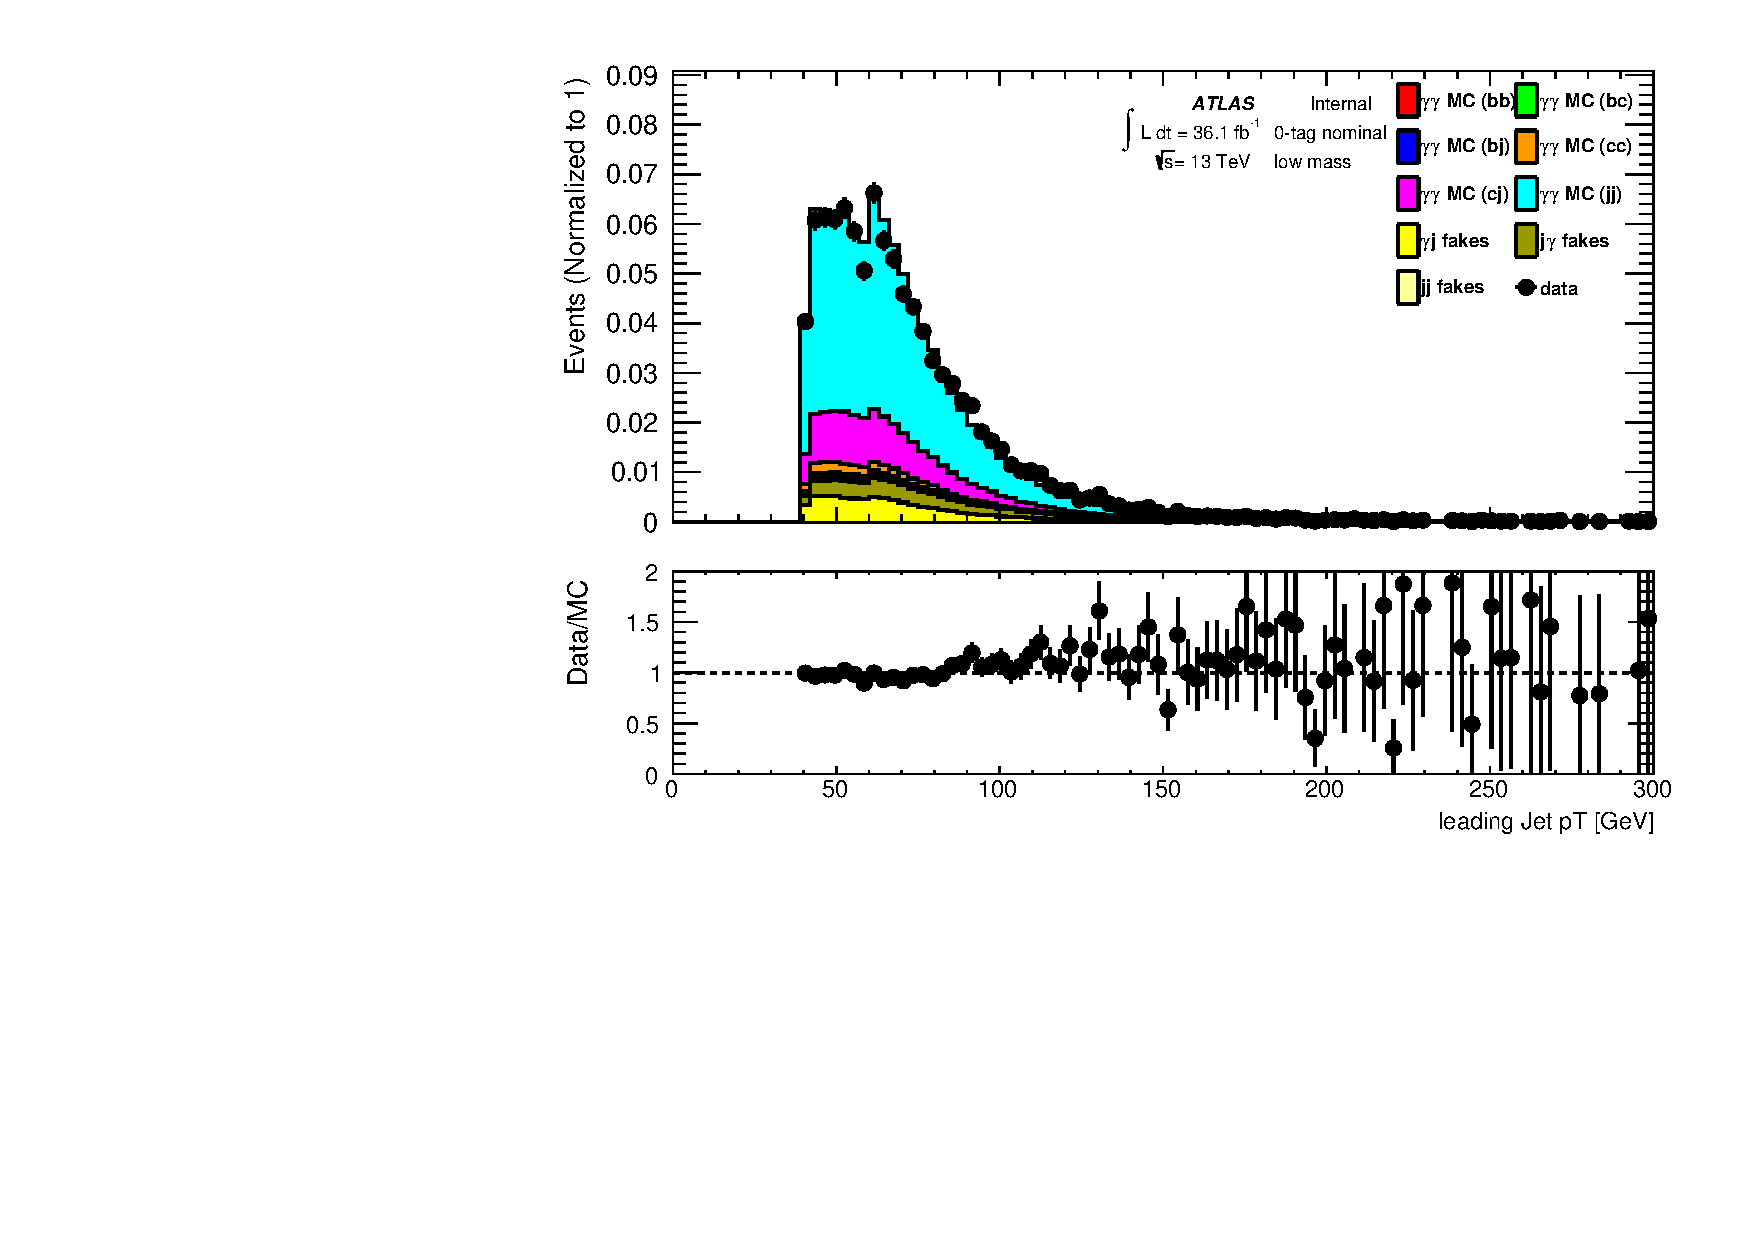
\includegraphics[width=0.48\textwidth]{chapters/chapter5_yybb/images/data_MC_comparison/h_CR_l_0t_nominal_leadingJet_pt.pdf}
  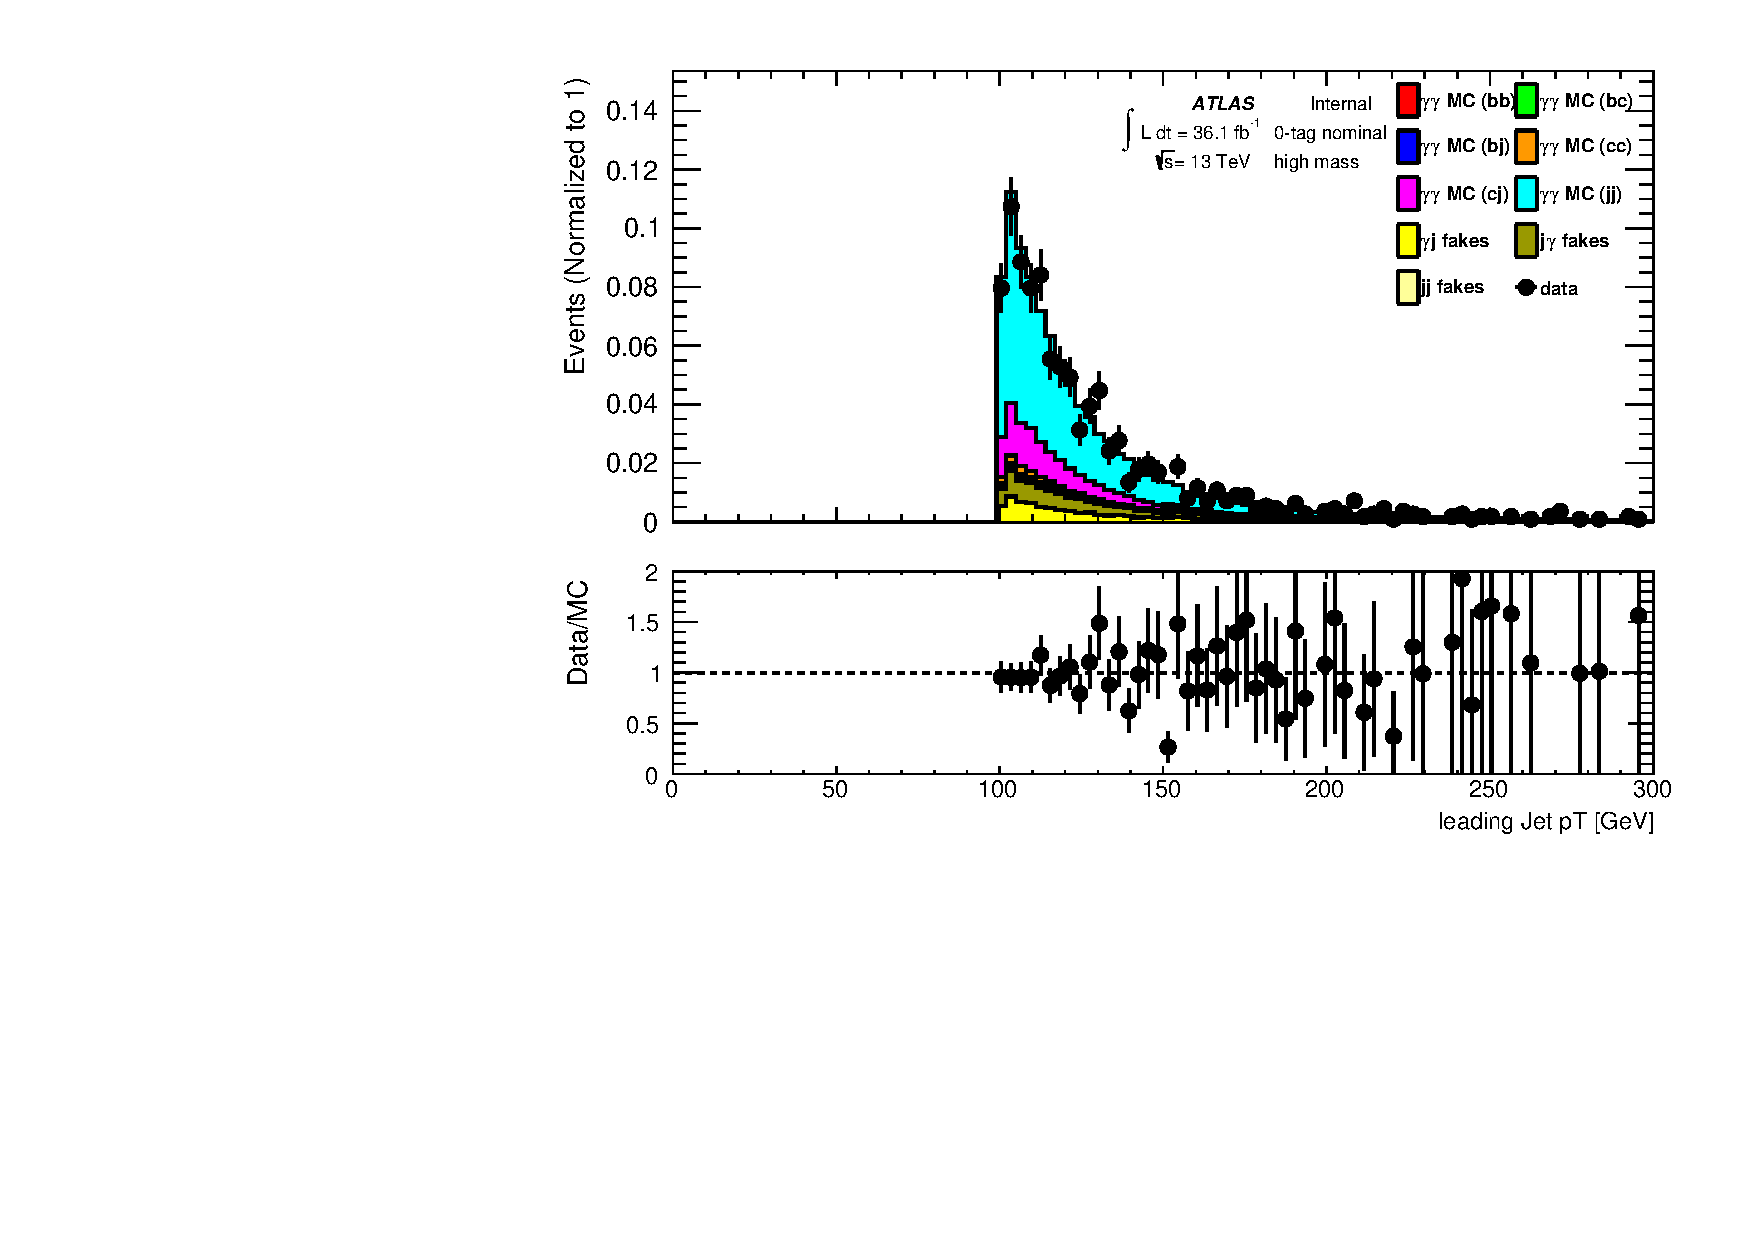
\includegraphics[width=0.48\textwidth]{chapters/chapter5_yybb/images/data_MC_comparison/h_CR_h_0t_nominal_leadingJet_pt.pdf}
  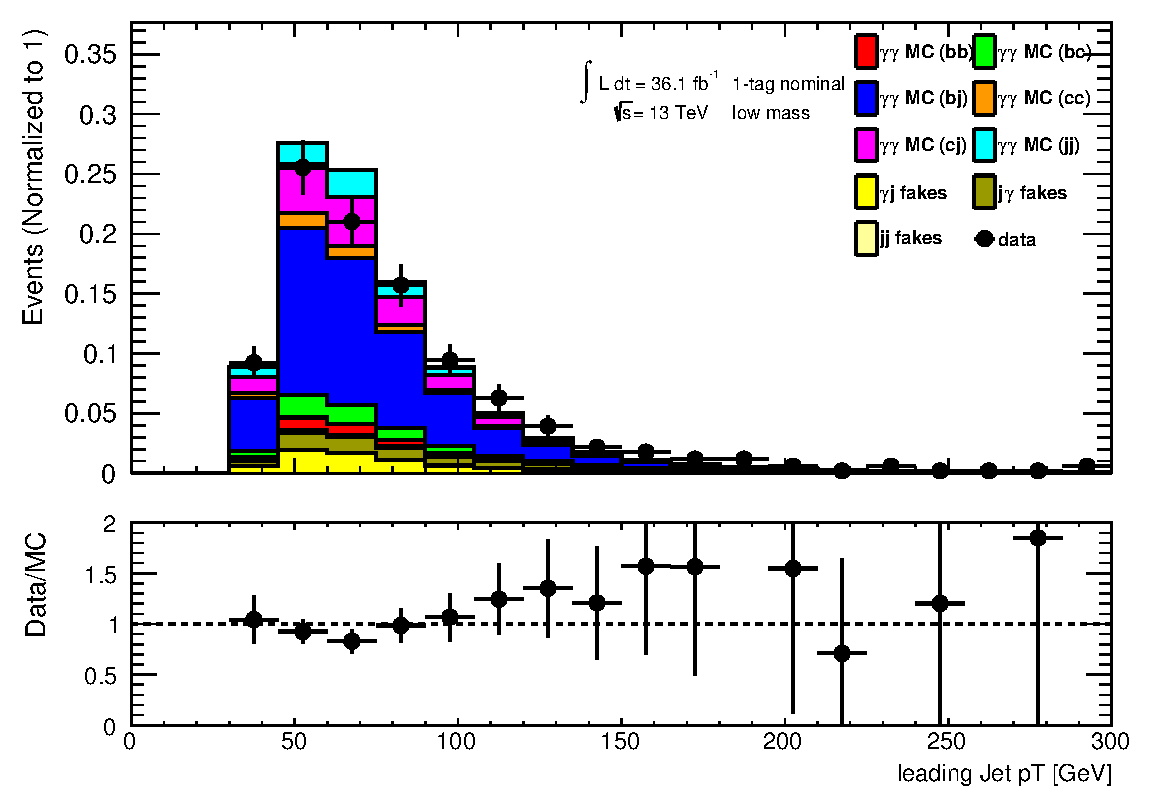
\includegraphics[width=0.48\textwidth]{chapters/chapter5_yybb/images/data_MC_comparison/h_SR_l_1t_nominal_leadingJet_pt.pdf}
  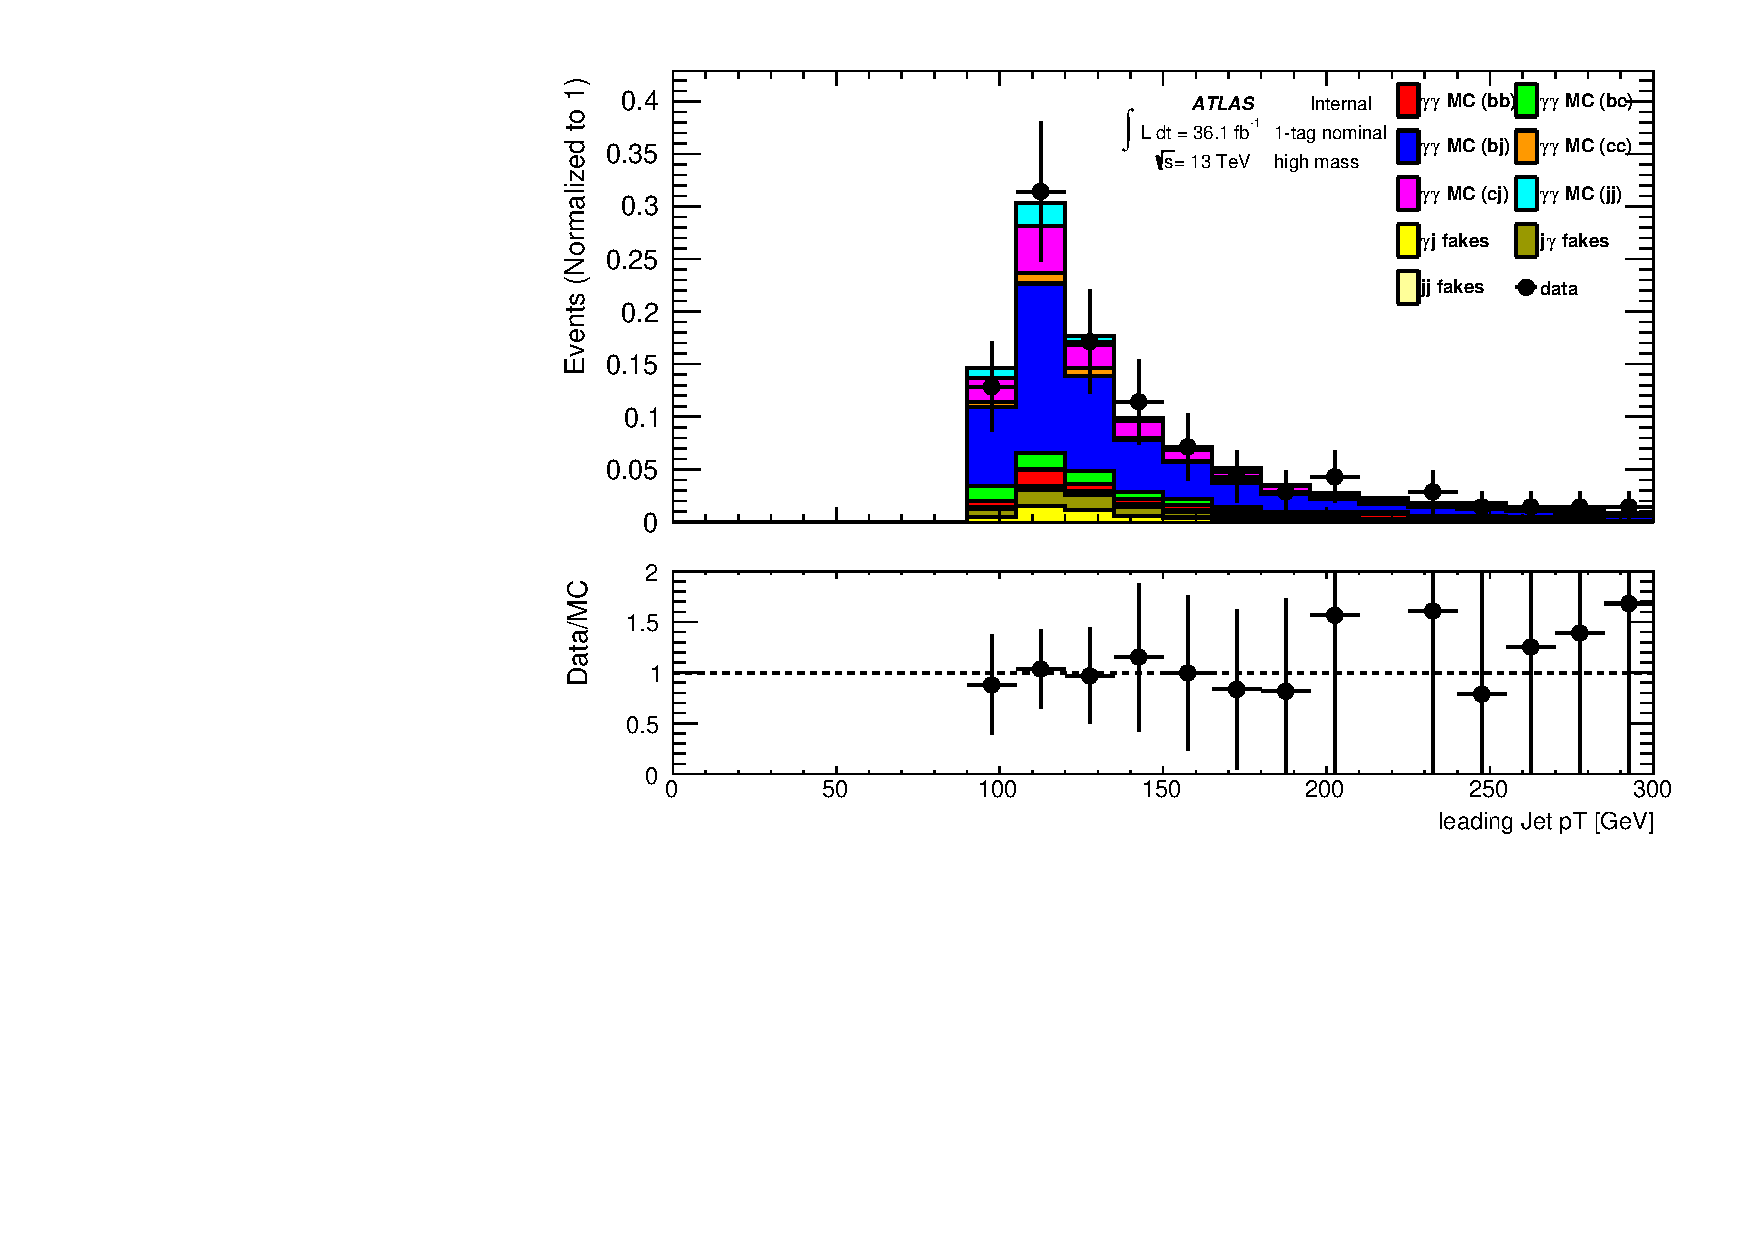
\includegraphics[width=0.48\textwidth]{chapters/chapter5_yybb/images/data_MC_comparison/h_SR_h_1t_nominal_leadingJet_pt.pdf}
  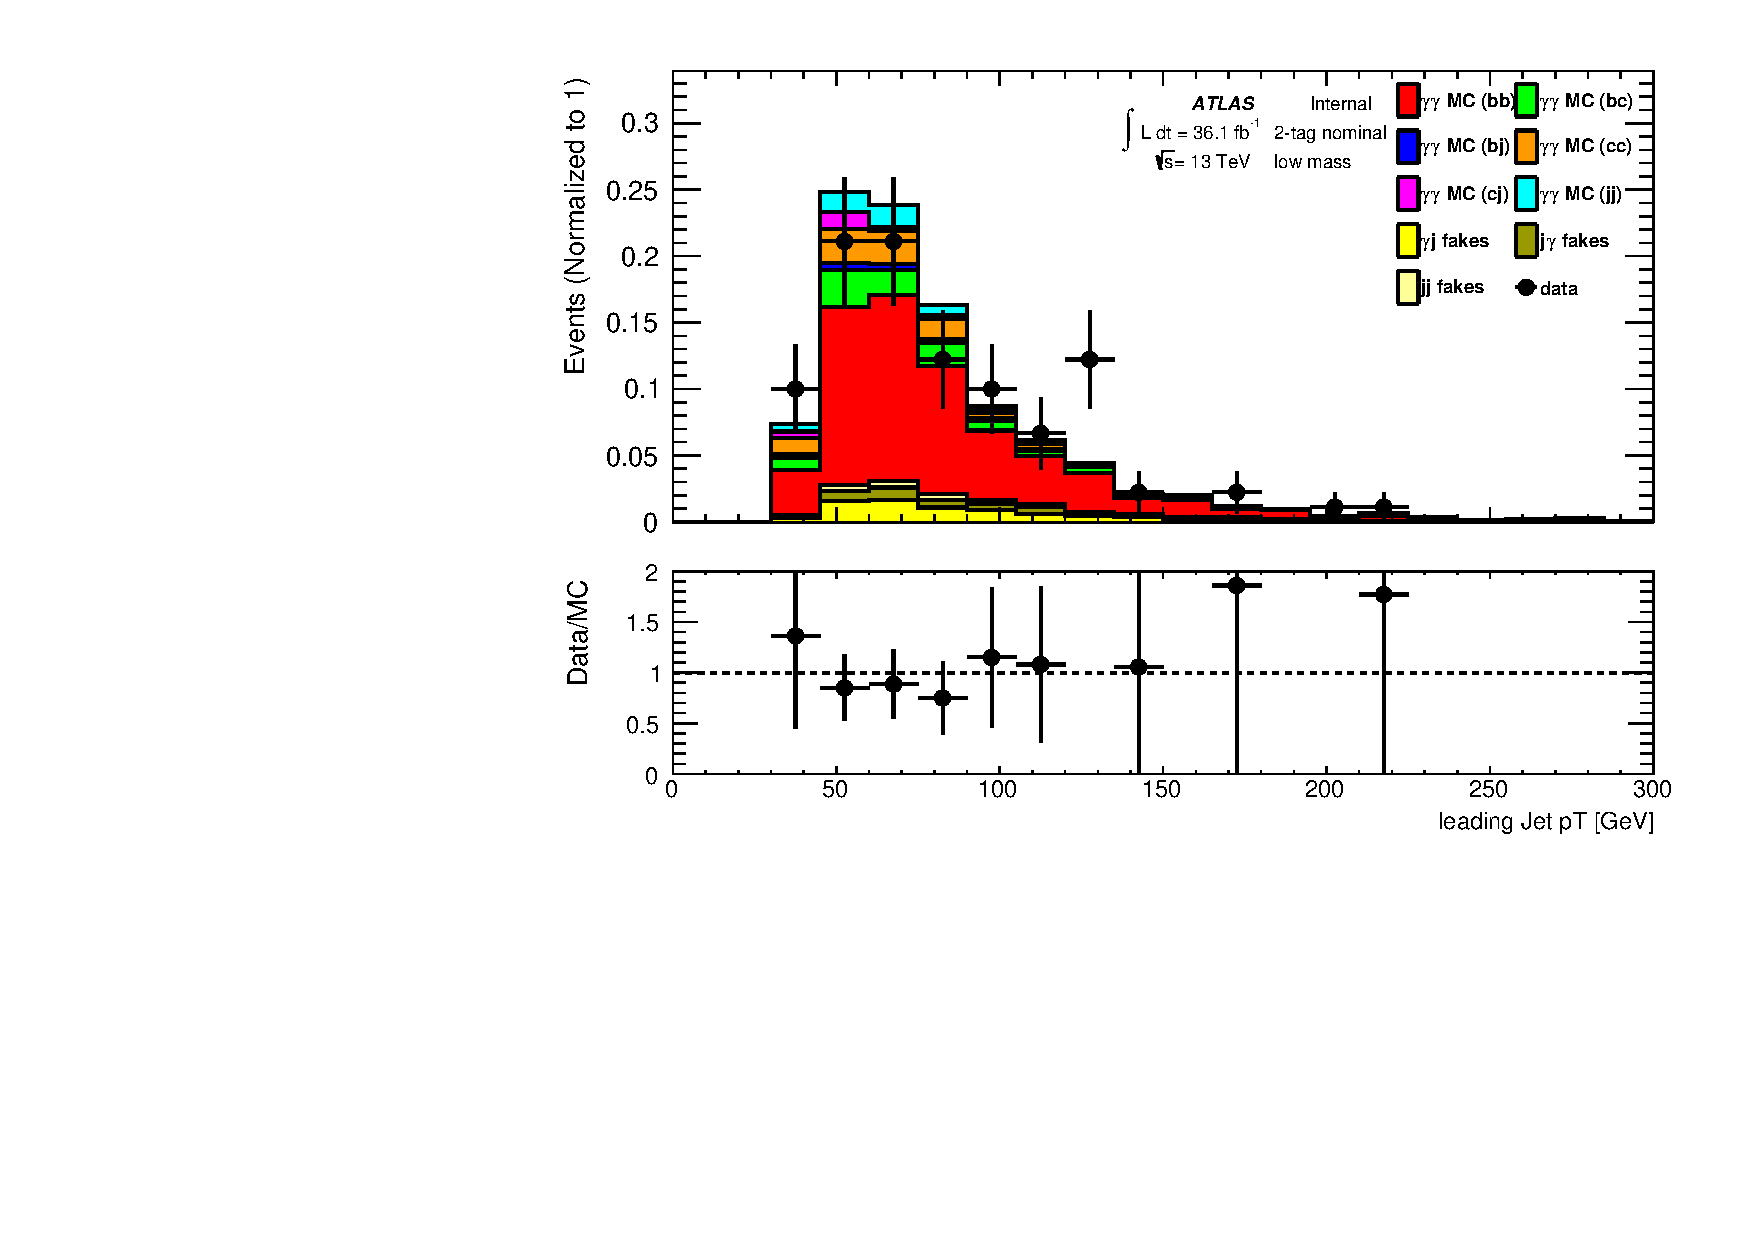
\includegraphics[width=0.48\textwidth]{chapters/chapter5_yybb/images/data_MC_comparison/h_SR_l_2t_nominal_leadingJet_pt.pdf}
  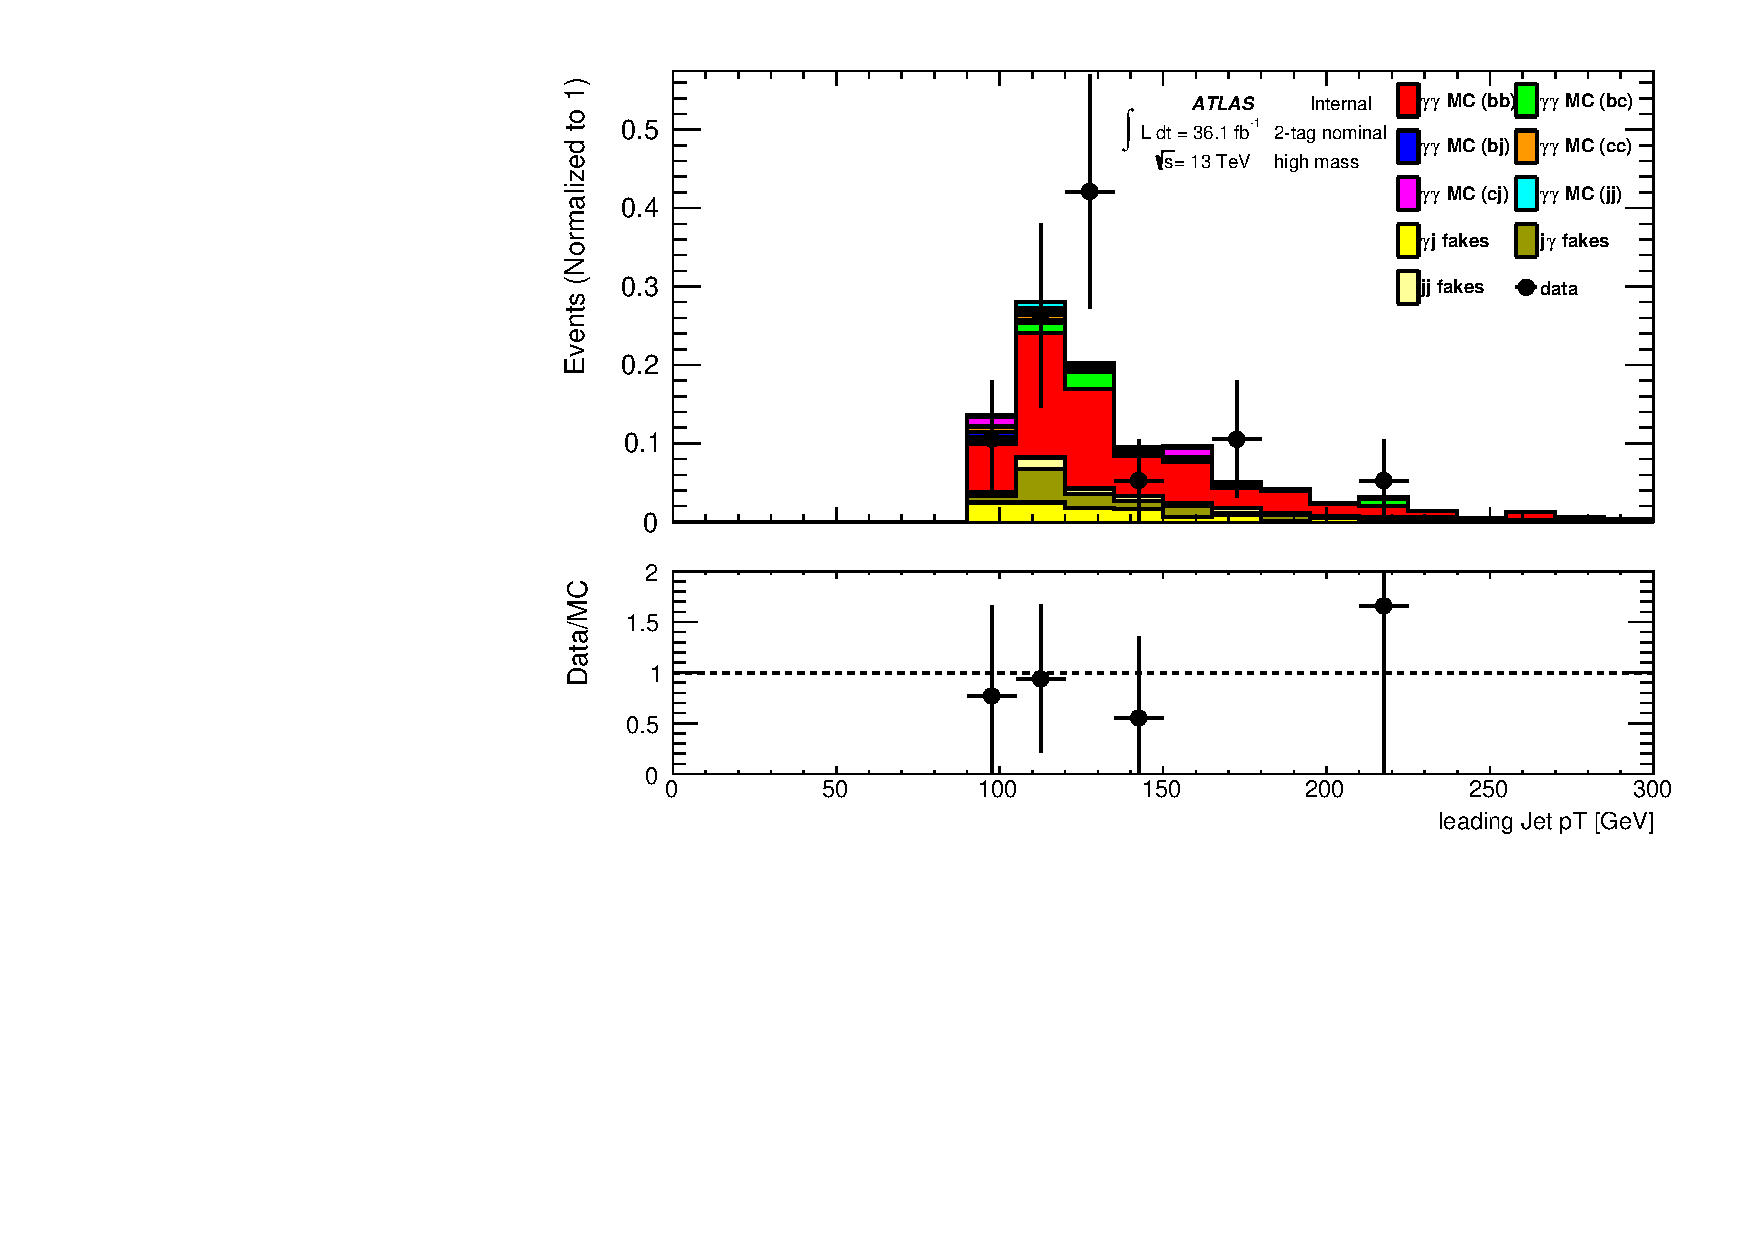
\includegraphics[width=0.48\textwidth]{chapters/chapter5_yybb/images/data_MC_comparison/h_SR_h_2t_nominal_leadingJet_pt.pdf}
  \caption[Leading jet \pt.]{Leading jet \pt by b-tagging category. The low (left) and high (right) mass selections are shown. Both data and MC are normalized such that the integral is 1.
  \label{fig:jet_l_pt}}
\end{figure}

\begin{figure}[htbp]
  \centering
  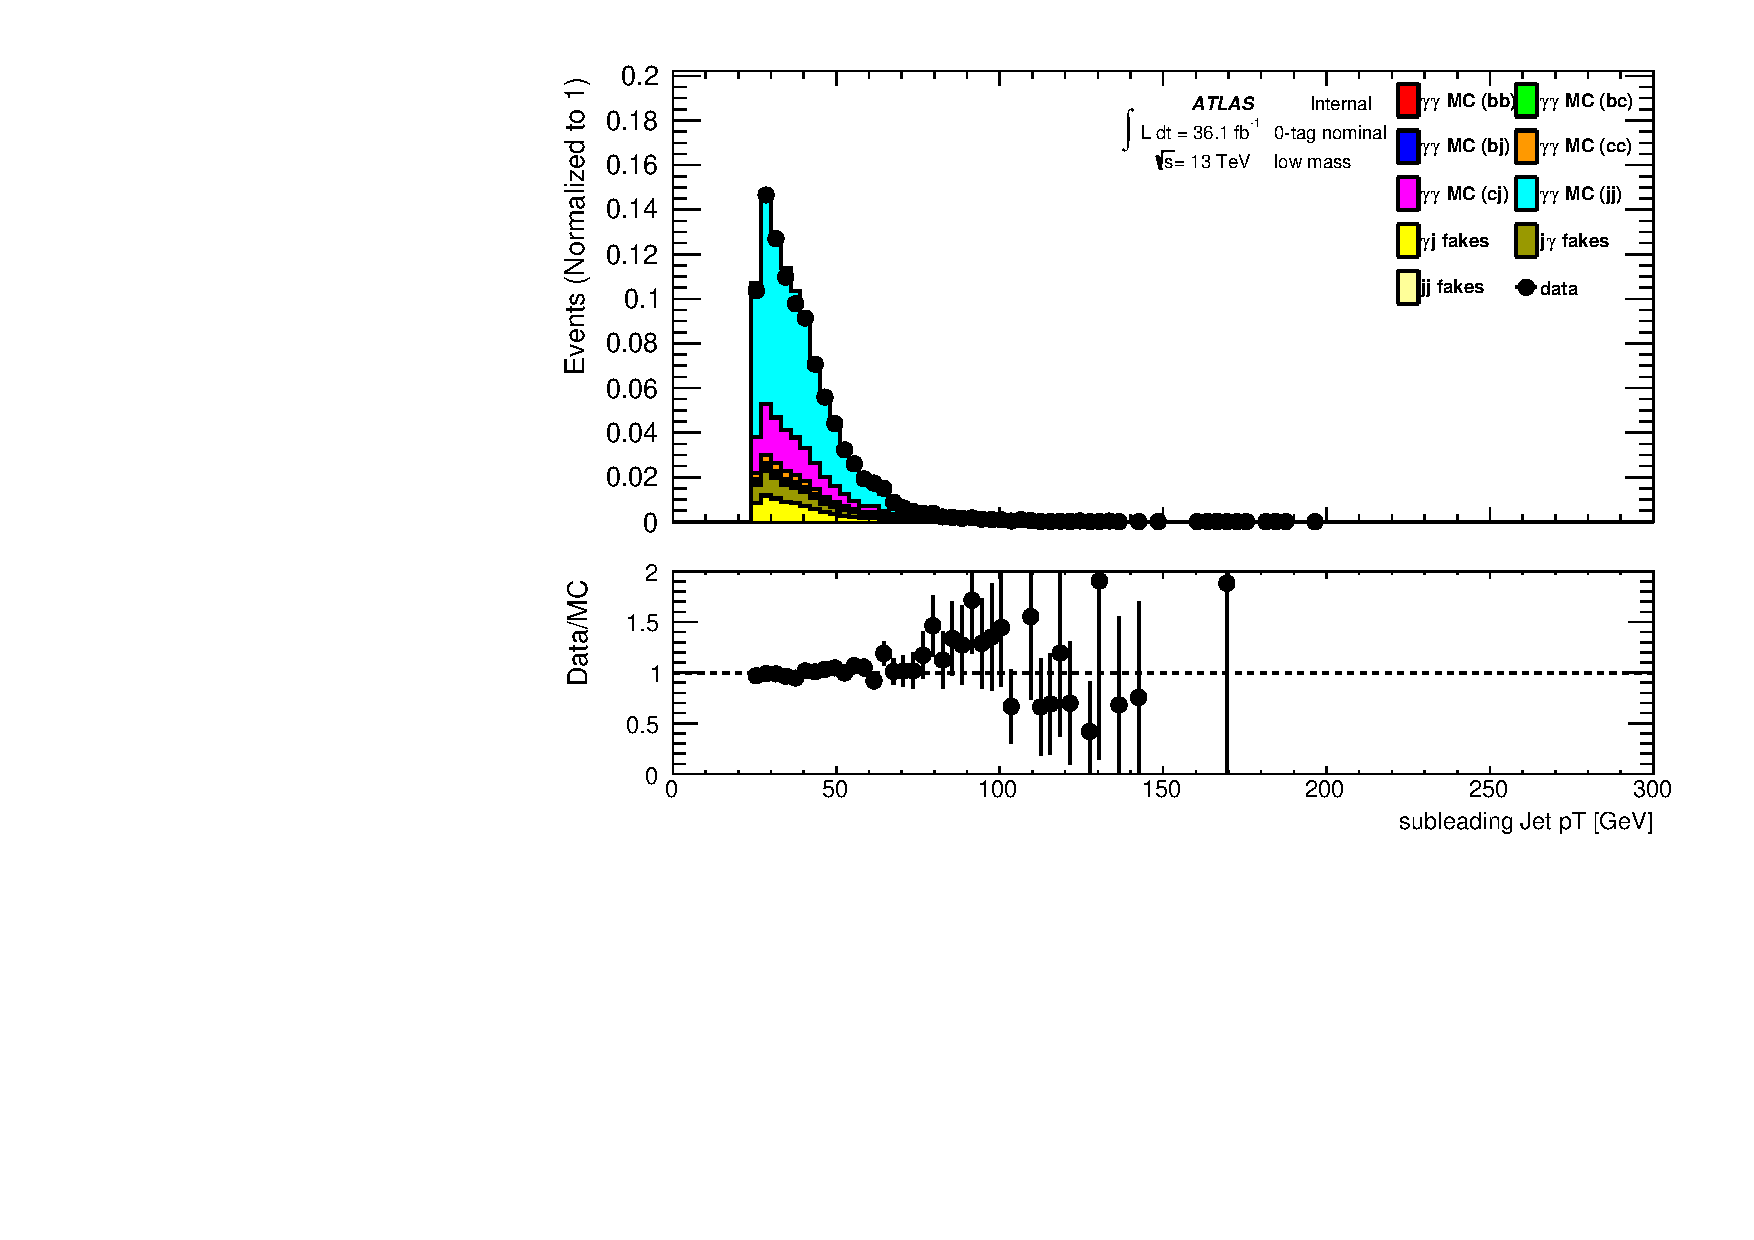
\includegraphics[width=0.48\textwidth]{chapters/chapter5_yybb/images/data_MC_comparison/h_CR_l_0t_nominal_subleadingJet_pt.pdf}
  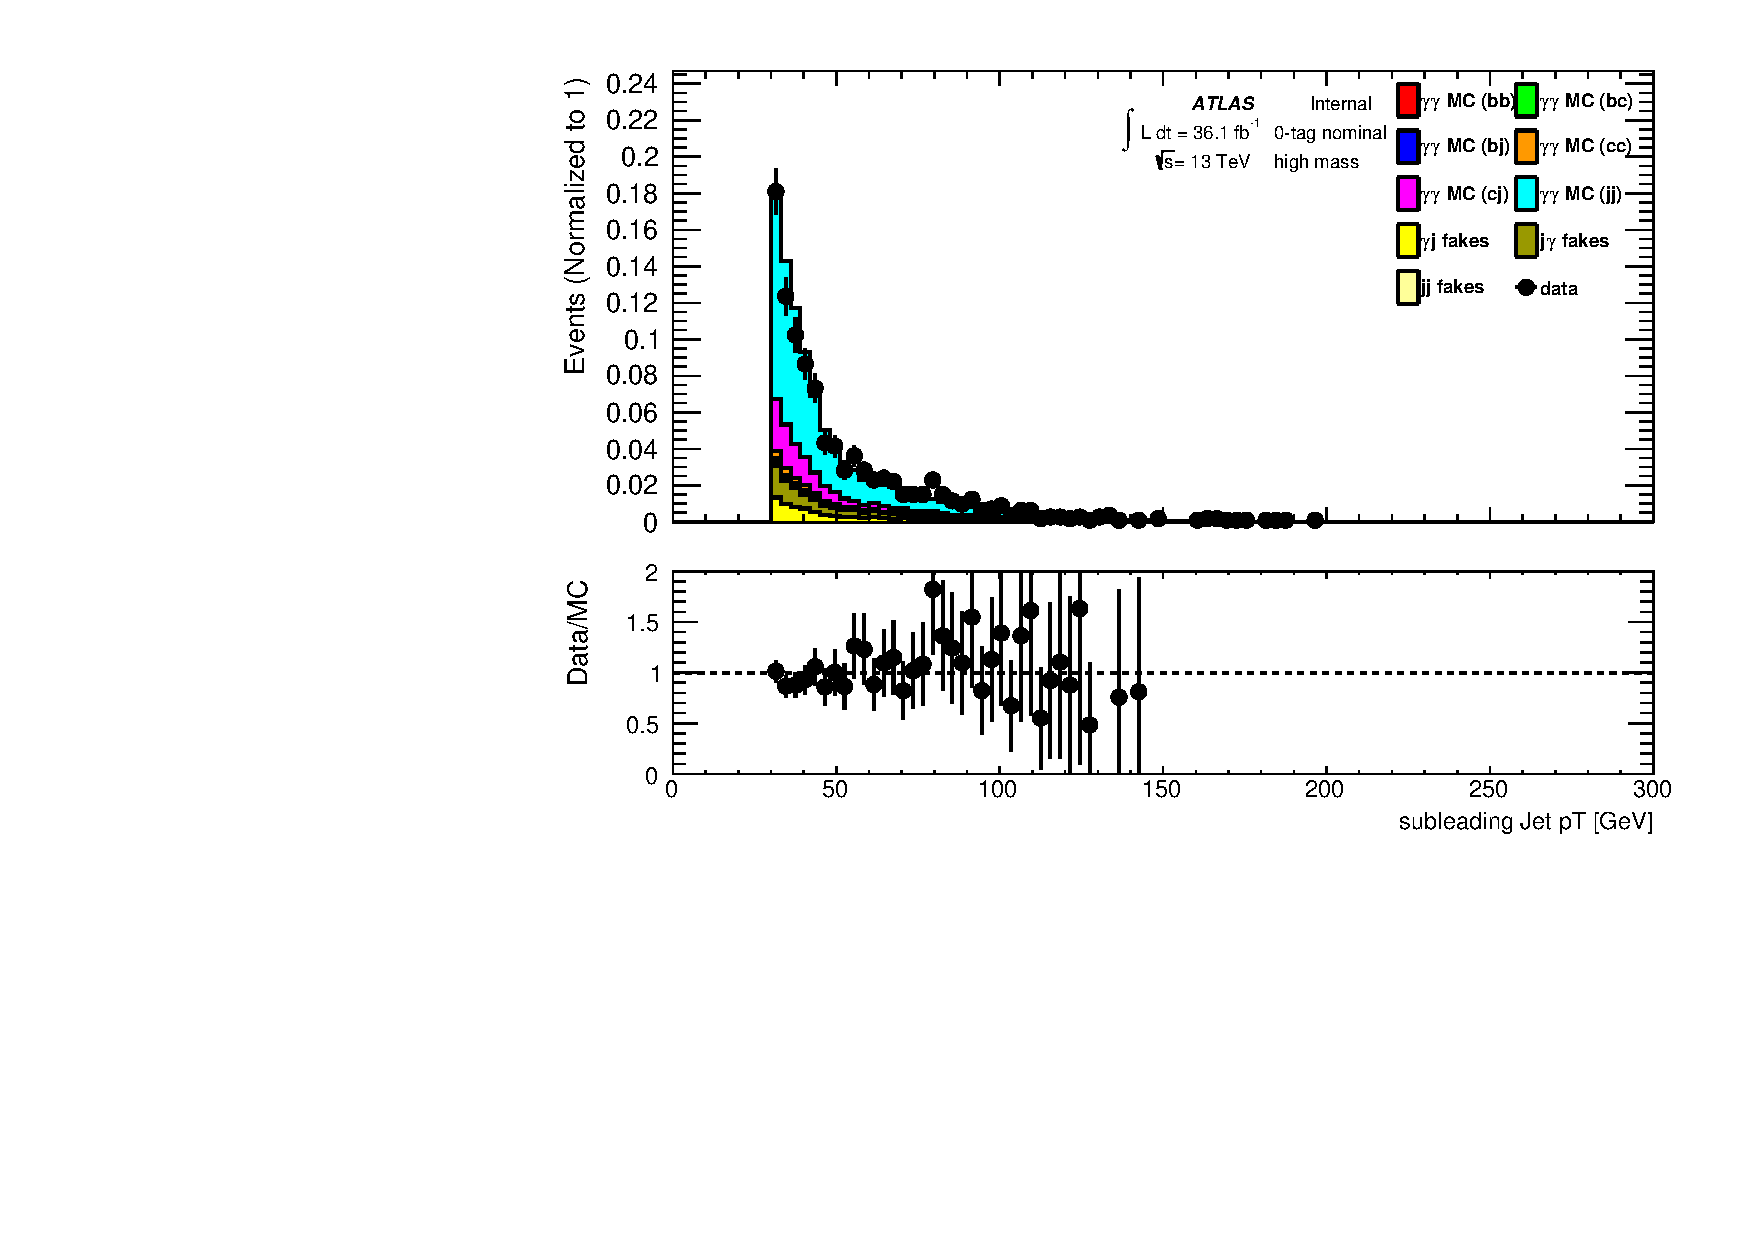
\includegraphics[width=0.48\textwidth]{chapters/chapter5_yybb/images/data_MC_comparison/h_CR_h_0t_nominal_subleadingJet_pt.pdf}
  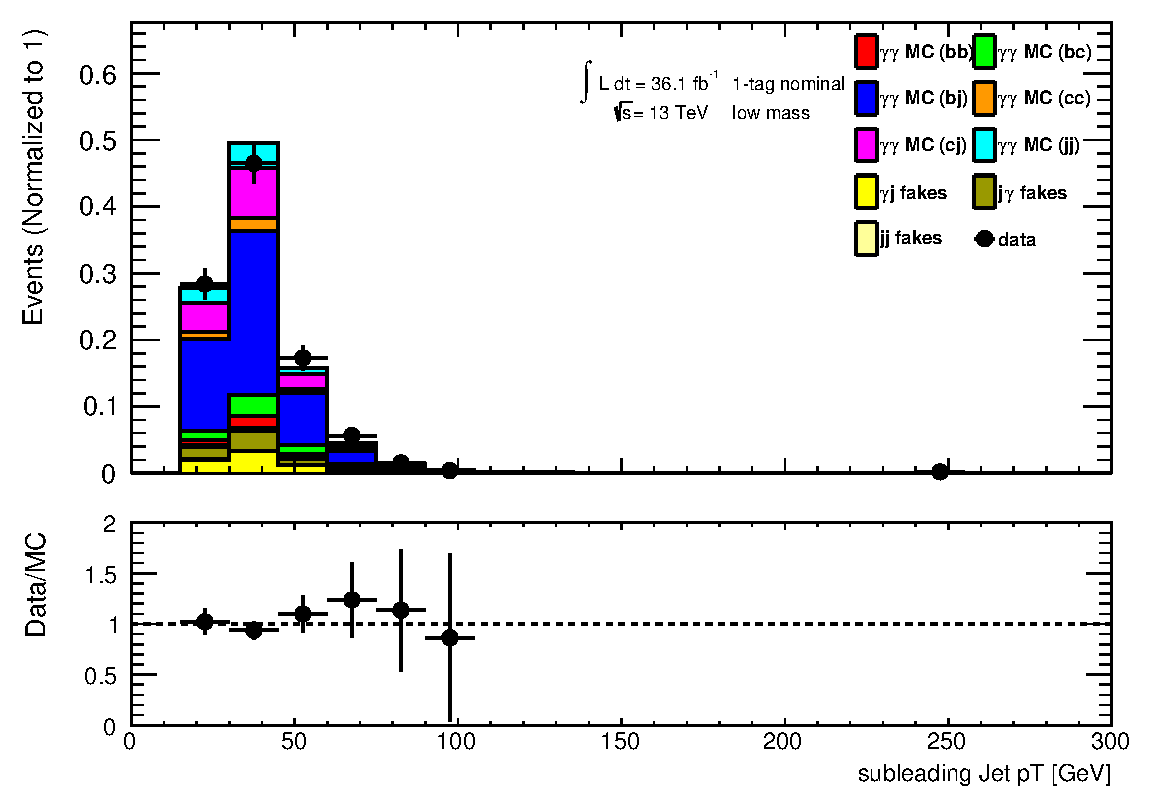
\includegraphics[width=0.48\textwidth]{chapters/chapter5_yybb/images/data_MC_comparison/h_SR_l_1t_nominal_subleadingJet_pt.pdf}
  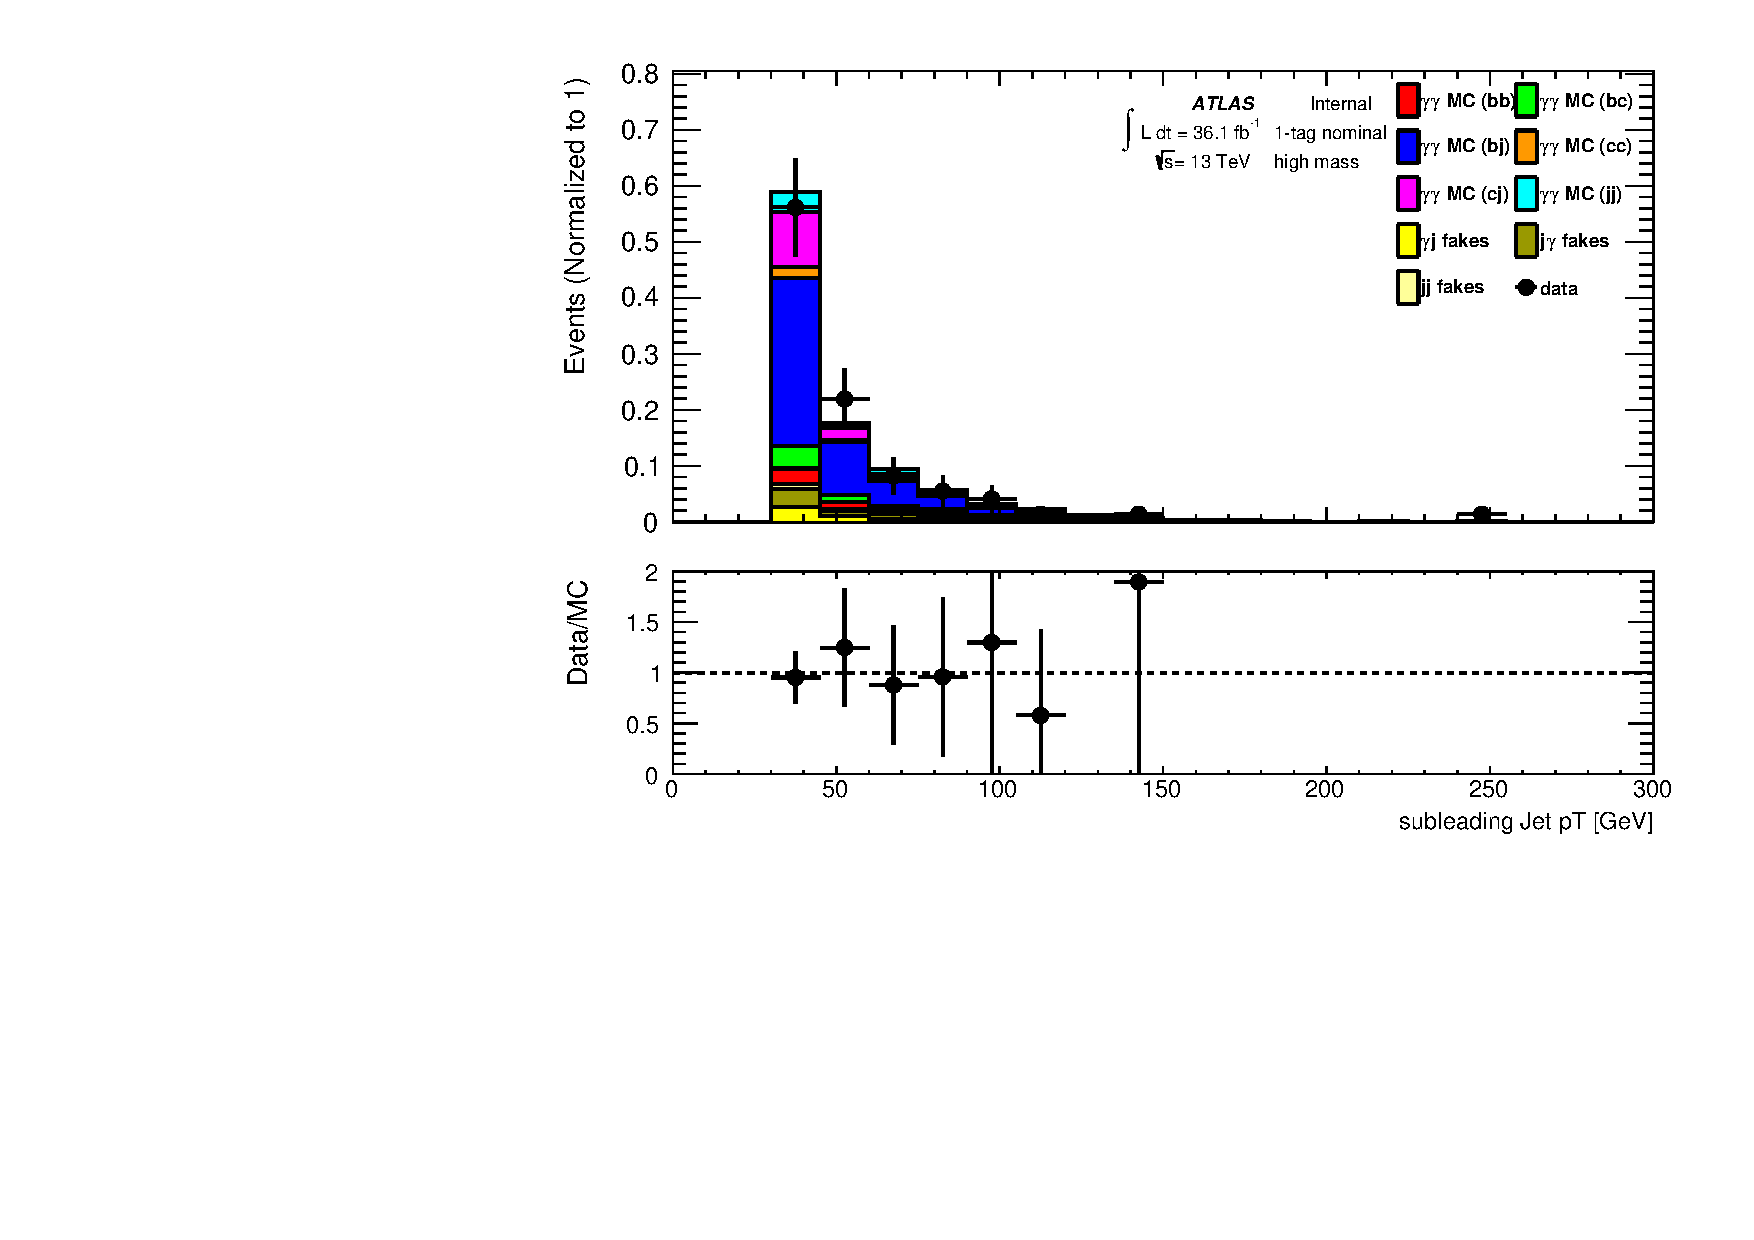
\includegraphics[width=0.48\textwidth]{chapters/chapter5_yybb/images/data_MC_comparison/h_SR_h_1t_nominal_subleadingJet_pt.pdf}
  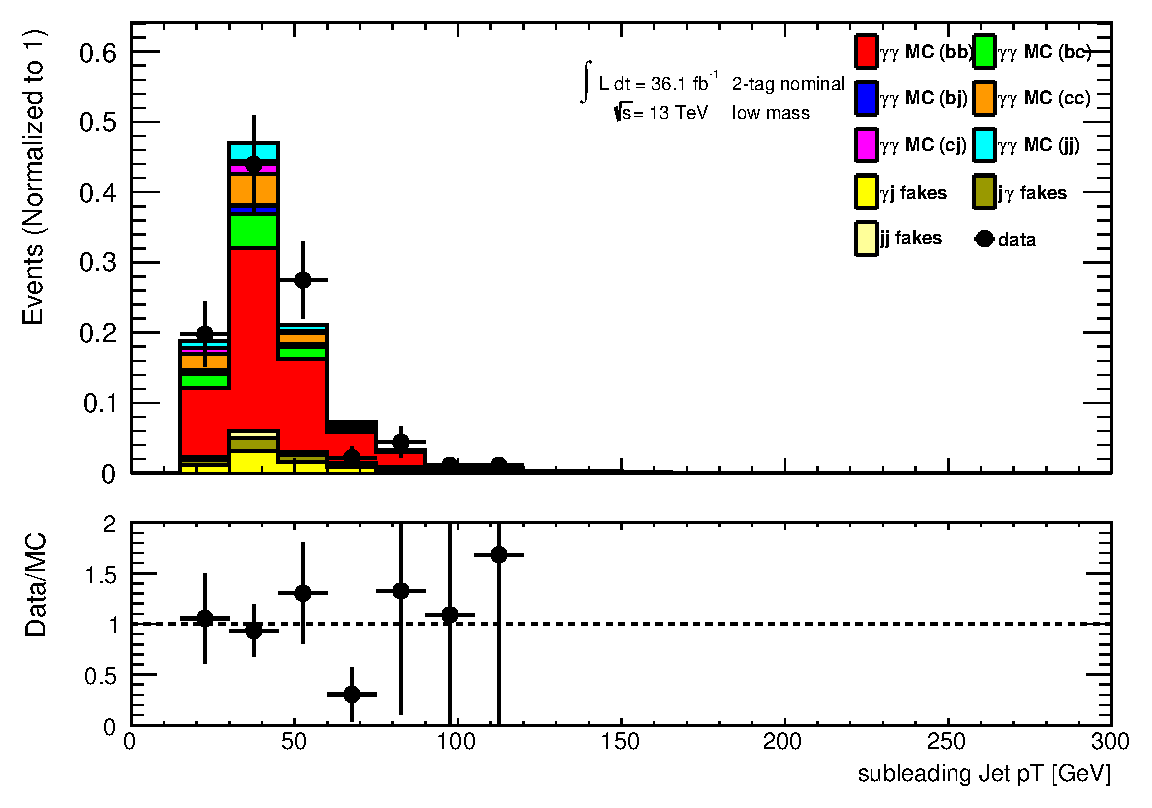
\includegraphics[width=0.48\textwidth]{chapters/chapter5_yybb/images/data_MC_comparison/h_SR_l_2t_nominal_subleadingJet_pt.pdf}
  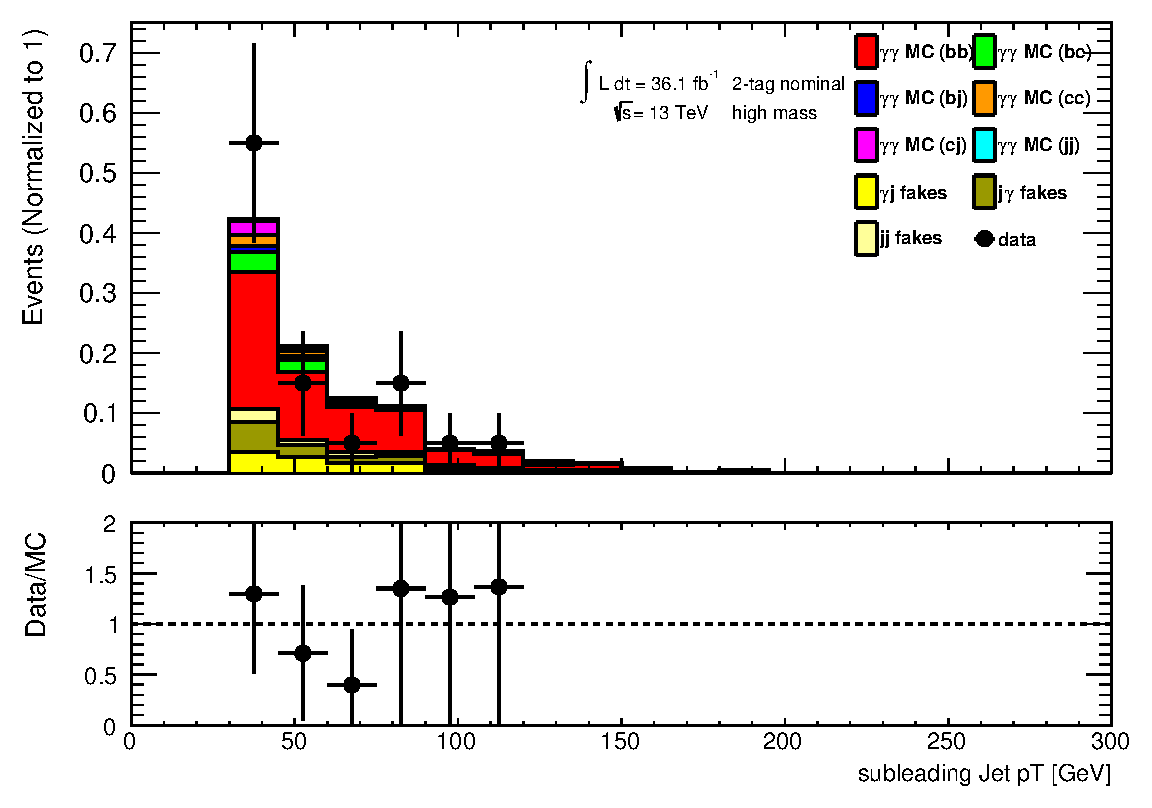
\includegraphics[width=0.48\textwidth]{chapters/chapter5_yybb/images/data_MC_comparison/h_SR_h_2t_nominal_subleadingJet_pt.pdf}
  \caption[Subleading jet \pt.]{Leading jet \pt by b-tagging category. The low (left) and high (right) mass selections are shown. Both data and MC are normalized such that the integral is 1.
  \label{fig:jet_s_pt}}
\end{figure}



\section{Event Selection}
\noindent\textbf{Preselection}\\
\indent For all samples, a preselection common to all \Hgg analyses is applied \cite{hgam-preselection}. To target this decay, events must pass the diphoton trigger, which requires two photons passing \textit{loose} identification. One of which must have $\et > \unit{35}{GeV}$ and the other must have $\et > \unit{25}{GeV}$. Nominally, this is the \path{g35_loose_g25_loose} trigger. After this trigger requirement, \pt cuts are applied, requiring the leading (subleading) photon \pt to be greater than 35\% (25\%) the diphoton invariant mass. Additionally the diphoton invariant mass must be in the window of 105 to 160 GeV.

A further requirement of two jets within the \btagging region ($\abseta <2.5$) is added to the preselection in order to target the \Hbb decay.

\noindent\textbf{Signal Selection}\\
\indent In addition to the preselection requirements, events are selected into 1 and 2-tag signal regions based on \btagging criteria. The 2-tag signal region requires exactly two jets passing the 70\% efficient \btagging \gls{WP}. If an event fails this requirement, but has one \bjet passing the 60\% efficient \btagging \gls{WP}, it is added to the 1-tag signal region.

Events with 3 jets passing the 70\% efficient \btagging \gls{WP} are vetoed from this analysis in order to maintain orthogonality with the $HH \rightarrow \bb \bb$ analysis.


For the resonant analysis, a scale factor is applied before reconstructing \myybb, rescaling the \bb system by a factor of $m_{H}/\mbb$ (with $m_H \equiv \unit{125.09}{\GeV}$) as a means to reduce the poor dijet resolution. This scaling improves the \myybb resolution as shown in Figure \ref{fig:resolution-myybb}.


\begin{figure}[htbp]
  \centering
  \subfloat[Low Mass, 1-tag selection]{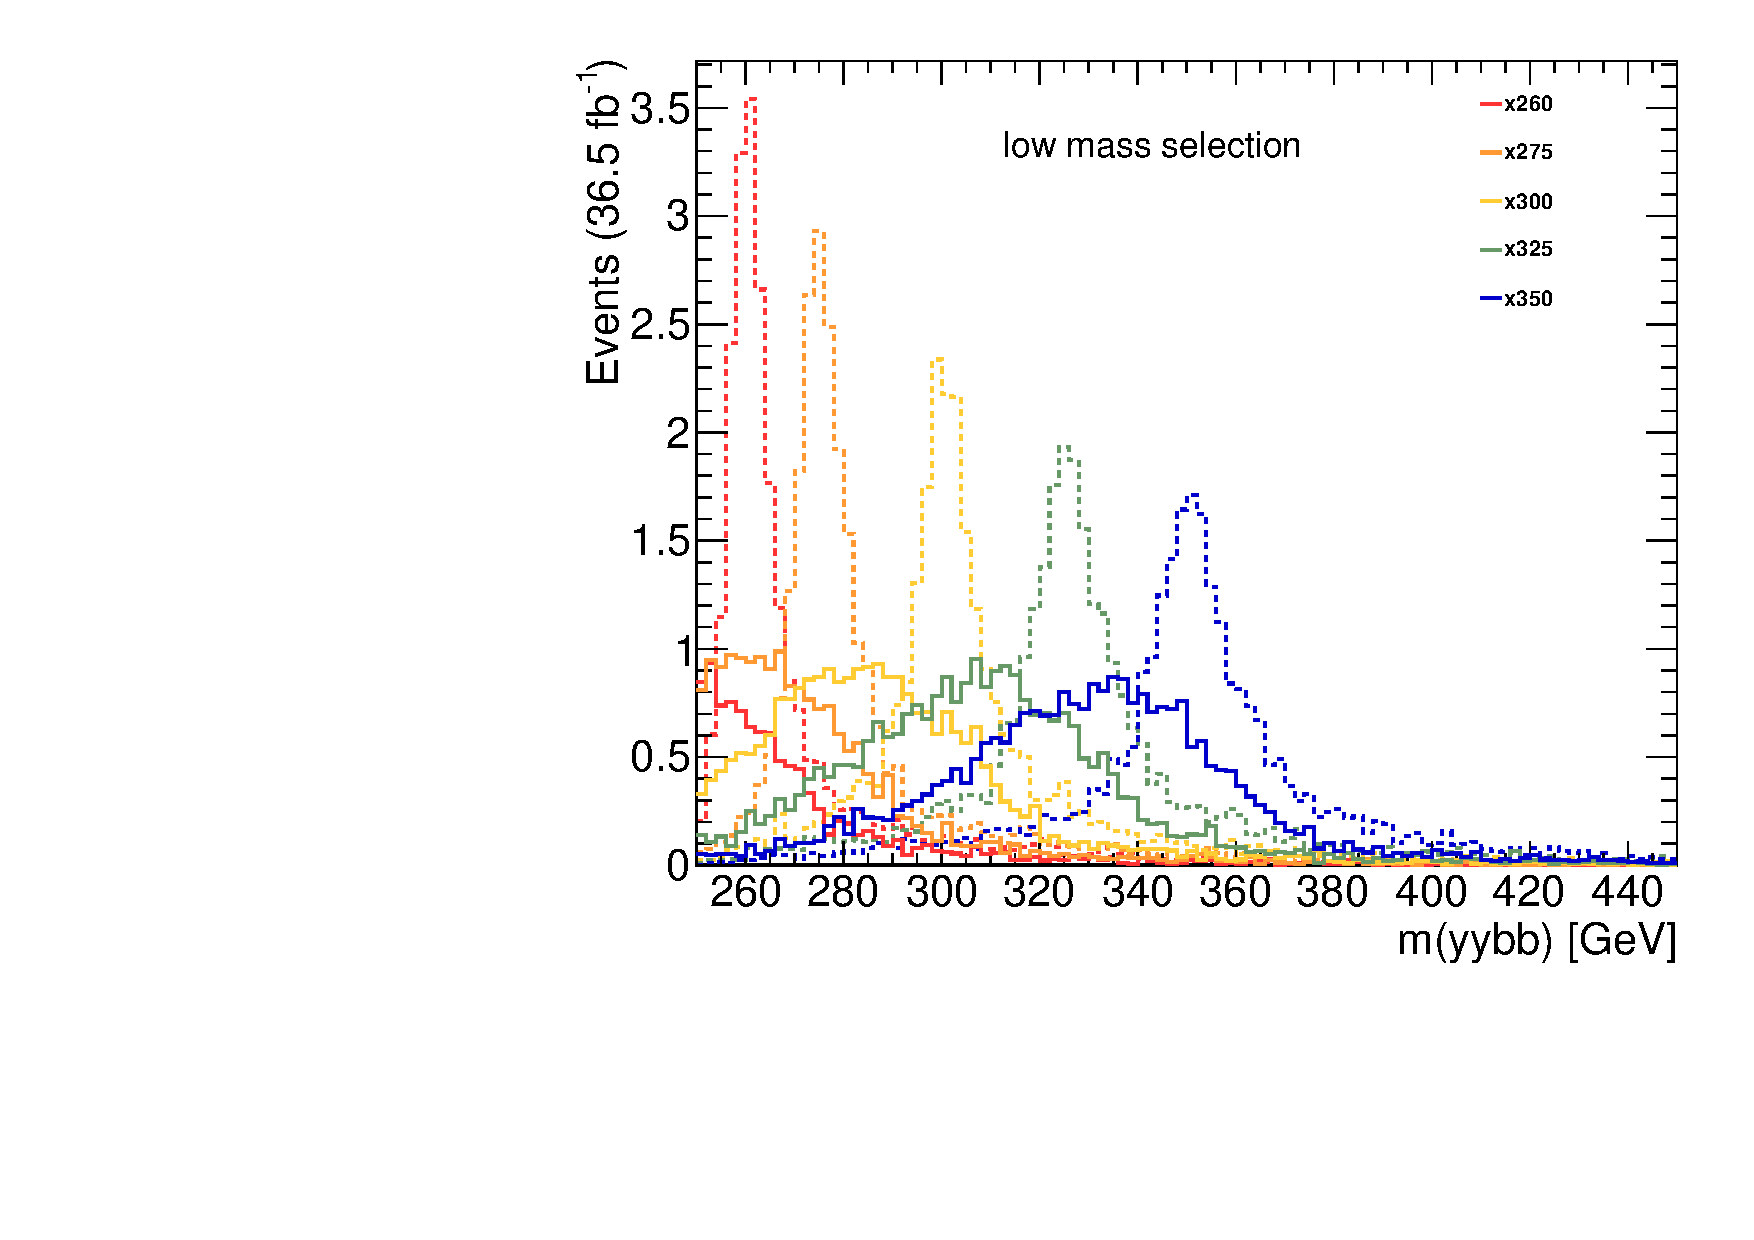
\includegraphics[width=0.48\textwidth]{chapters/chapter5_yybb/images/selection/m_yybb_low_1.pdf}}
  \subfloat[High Mass, 1-tag selection]{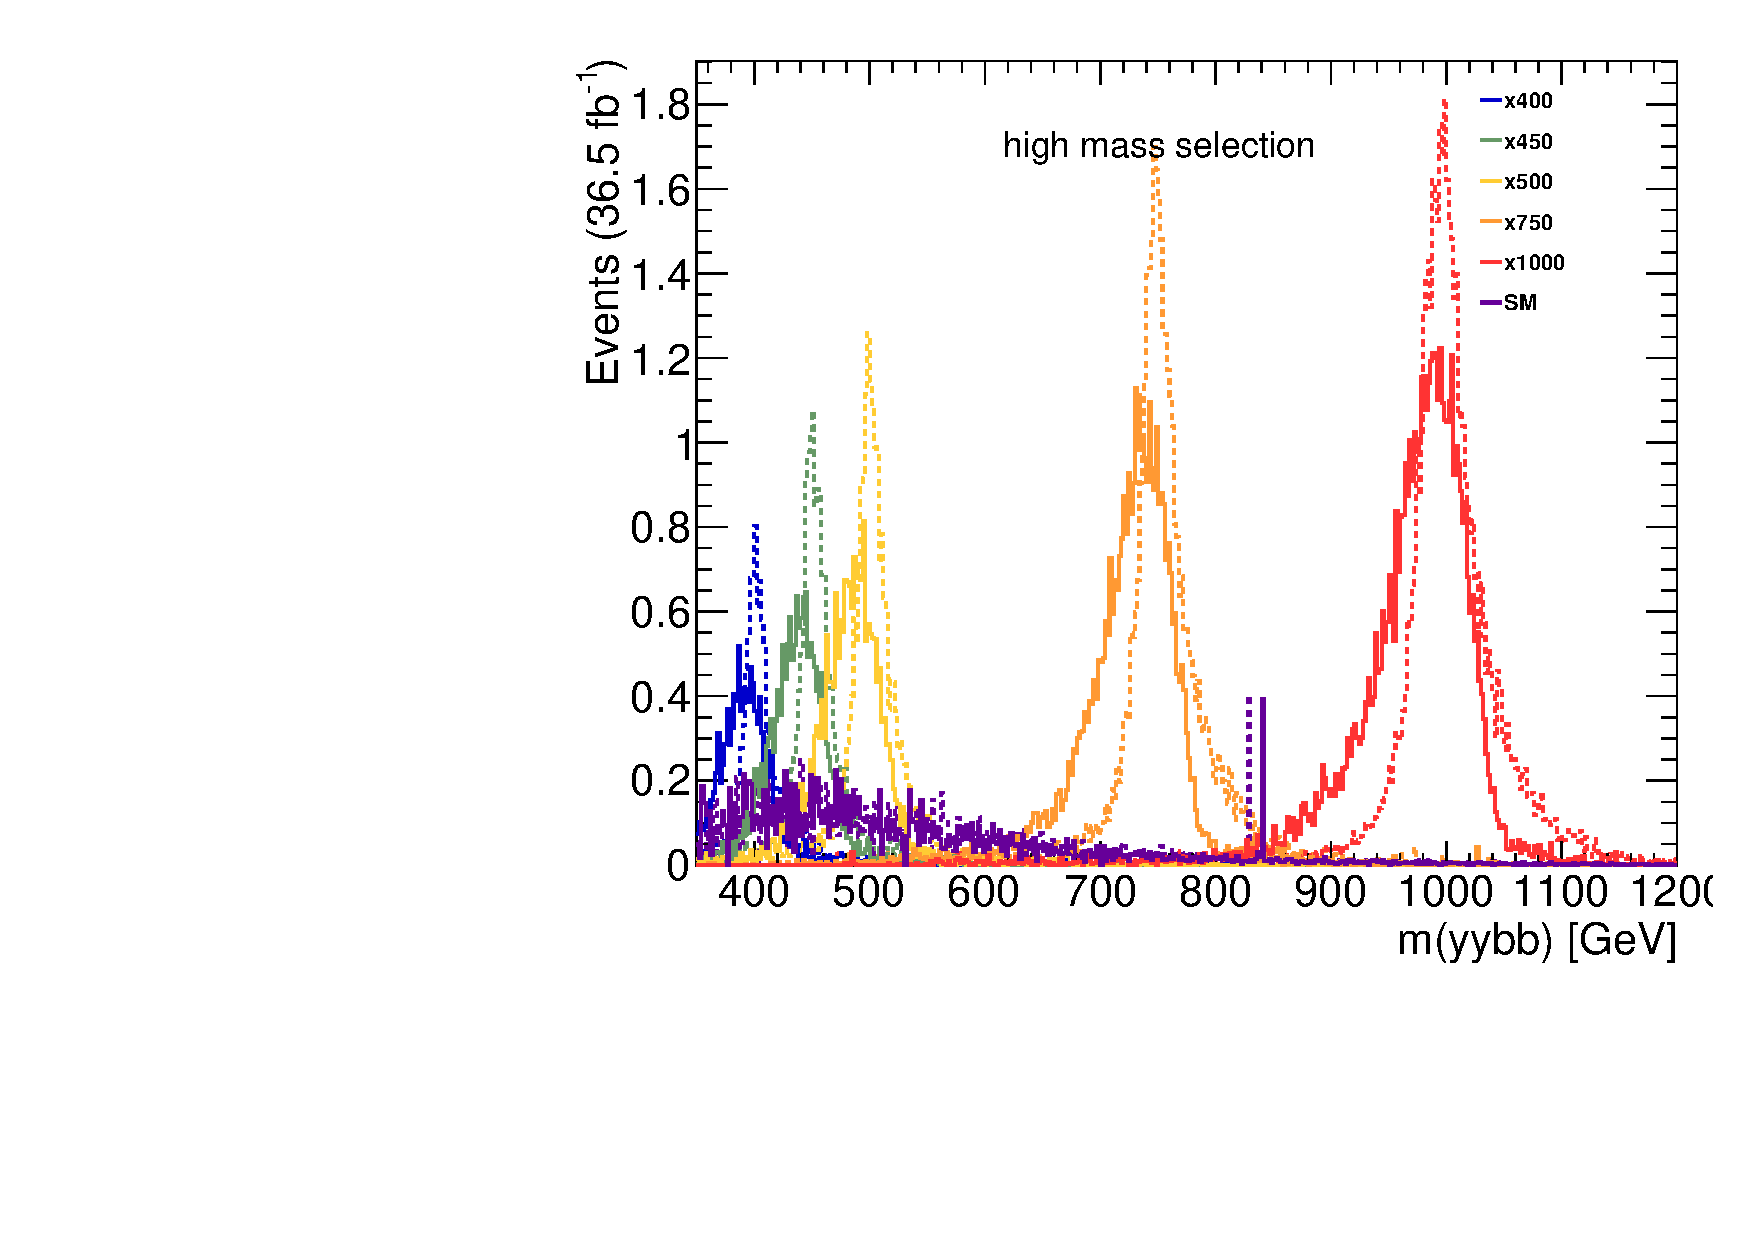
\includegraphics[width=0.48\textwidth]{chapters/chapter5_yybb/images/selection/m_yybb_high_1.pdf}}\\
  \subfloat[Low Mass, 2-tag selection]{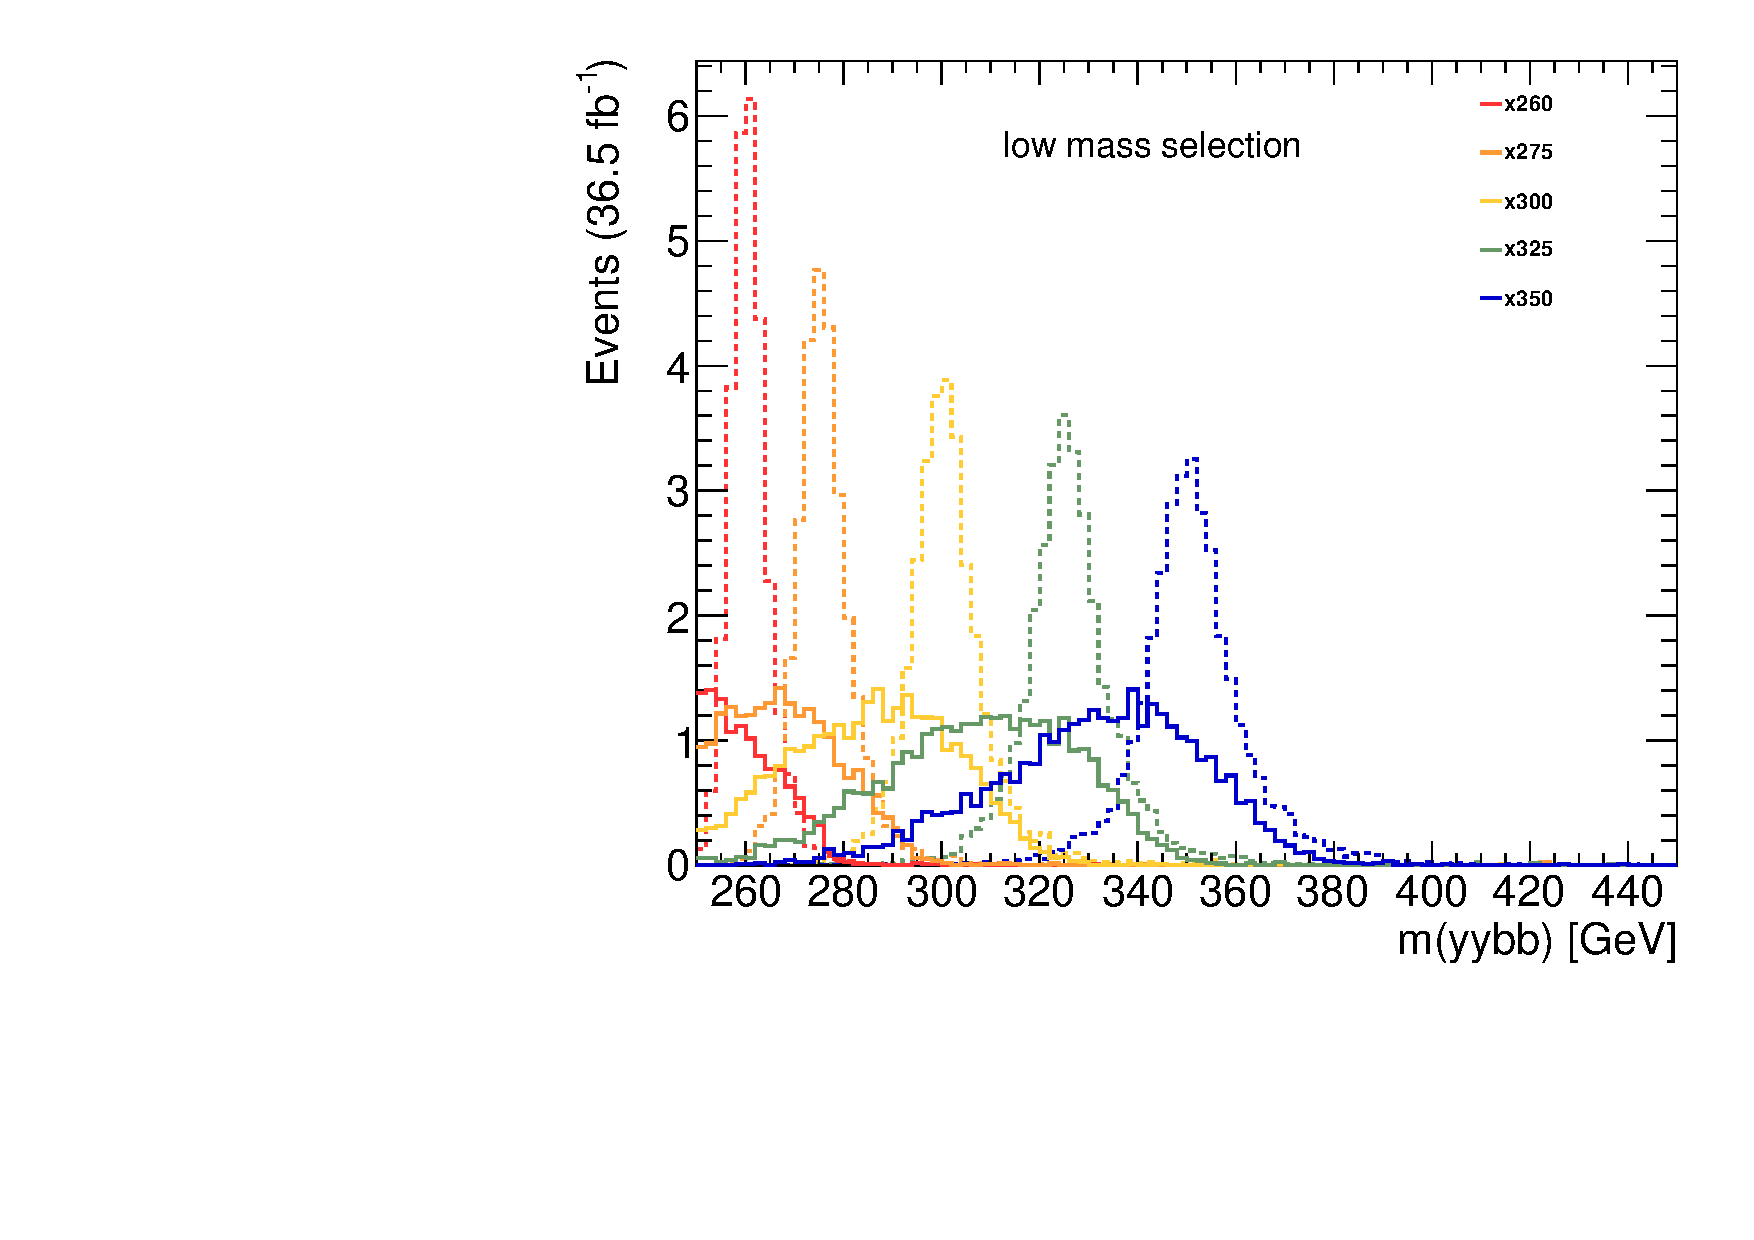
\includegraphics[width=0.48\textwidth]{chapters/chapter5_yybb/images/selection/m_yybb_low_2.pdf}}
  \subfloat[High Mass, 2-tag selection]{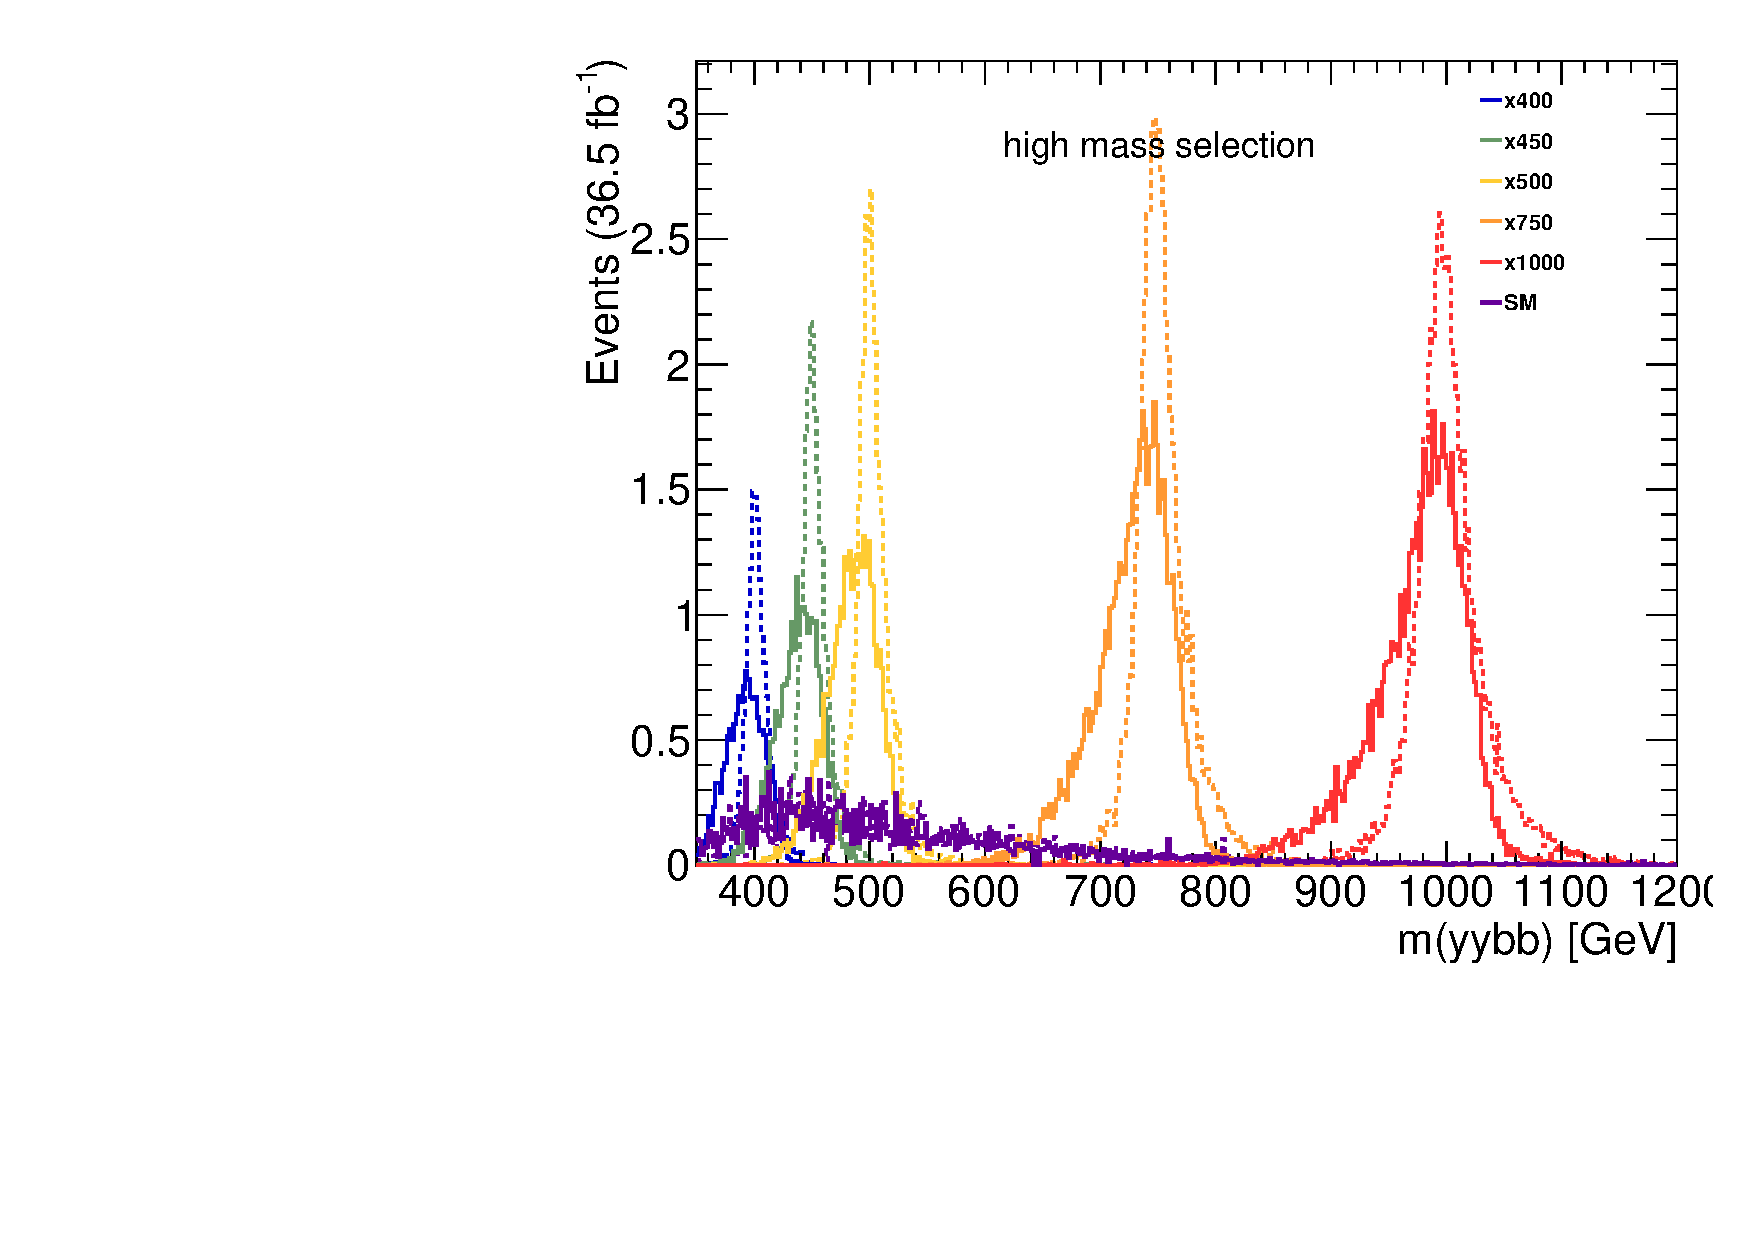
\includegraphics[width=0.48\textwidth]{chapters/chapter5_yybb/images/selection/m_yybb_high_2.pdf}}
  \caption[Reconstructed \myybb for the signal \gls{MC} samples, with and without the dijet mass constraint]
  {Reconstructed \myybb for the signal \gls{MC} samples. The solid lines show the distribution before applying the dijet mass constraint, the dashed lines have the dijet mass constraint imposed. Low and High, 1 and 2-tag selections are shown.}
  \label{fig:resolution-myybb}
\end{figure}



\section{Modeling}



\subsection{Non-resonant Analysis}
\subsubsection{Signal Modeling}

A double-sided Crystal Ball function \cite{dscb-diphoton}, a Gaussian core with power-law tails, is used to describe the shape of the \hhyybb signal. Model parameters are taken from the simulated signal sample.

\subsubsection{Background Modeling} \label{sssec:nonres-bkg-model}

The background for the non-resonant analysis is composed of a model for the smoothly-falling \yy-continuum, and a model for single Higgs boson production. 


For the \yy-continuum background, a functional form is fit to data. The fit function is selected through a \textit{spurious signal} test \cite{spurious-signal-diphoton}, which evaluates potential bias from this procedure. This test performs signal-plus-background fits to just the simulated background, evaluating the extracted signal in the $\unit{121}{\GeV} < \myy < \unit{129}{\GeV}$ window, which is taken as the bias. This procedure is repeated for each considered function, and the function with the fewest spurious signal events is selected as the background function. If functions have the same bias, then by an Occam's Razor argument, the function with fewer free parameters is selected.

The considered functions for this test are as follows:
\begin{itemize}
  \item Exponential, consider orders $N=1,2,3$. Generalized form: $Exp^N (\myy ; \theta^{bkg}) = exp(\sum\limits_{j=0}^{N} \theta_j^{bkg} \dot m_{\gamma\gamma}^j)$
  \item Bernstein, consider orders $N=3,4,5$. Generalized form: $Bernstein^N (\myy ; \theta^{bkg}) = \sum\limits_{j=0}^{N} \theta_j^{bkg} b_{j,N}$, for $b_{j,N} = C_n^i x^j (1-x)^{N-j}$, where $x= (\myy-100)/60$
  \item Dijet of form: $dijet(\myy ; \theta^{bkg}) = \theta_1^{bkg} (1-\myy)^{\theta_2^{bkg}} m_{\gamma\gamma}^{\theta_3^{bkg}}$
\end{itemize}

Through this test, the first-order exponential function is found to have the lowest bias, and is selected as the \yy-continuum background model.

The single Higgs boson background is modeled through a double-sided Crystal Ball function, where parameters are taken from simulation.

\subsection{Resonant Analysis}
\subsubsection{Signal Modeling}

For the resonant analysis, the signal is modeled by a function using a gaussian core, with exponential tails, known as \texttt{ExpGaussExp}\footnote{Also, ``double-shouldered GaussExp''} \cite{exp-gauss-exp}. This function is fit in a window around the mass hypothesis. %TODO: More here


\subsubsection{Background Modeling} \label{sssec:res-bkg-model}

A spurious signal test (described in Section \ref{sssec:nonres-bkg-model}) is performed

For the loose selection in the low mass region, a Novosibirsk function \cite{novosibirsk} is selected, which has the generalized form:

\begin{equation}
  \begin{split}
  P(x) &= exp(-0.5^{ln(q_y)^2 / \Lambda^2 + \Lambda^2})\\
  \text{with,} \quad \quad q_{y} &= 1 + \Lambda(x-x_0)/\sigma \times \frac{\sinh(\Lambda \sqrt{\ln(4)})}{\Lambda \sqrt{\ln(4)}}
  \end{split}
\end{equation}

The Novosibirsk function features a peak at low value, followed by a smoothly falling tail. For the tight selection, used in the high mass region, an exponential function is selected.

\section{Systematic Uncertainties}

As a result of the small \hh cross-section, the sensitivity of this analysis is dominated by statistical uncertainties\footnote{The statistical uncertainties are taken as Poisson uncertainties ($1/\sqrt{N}$).}. The following sections will discuss systematic uncertainties, both theoretical (Section \ref{ssec:theory-unc}) and experimental (Section \ref{ssec:theory-unc}).

\subsection{Theoretical Uncertainties} \label{ssec:theory-unc}

This section describes theoretical uncertainties on the mono-Higgs and di-Higgs samples. In each of these, alternate models of parton showering and hadronization were considered and differences were found to be negligible.

\noindent\textbf{Mono-Higgs:} Theory uncertainties for the mono-Higgs boson production cross-section are estimated through varying renormalization and factorization scales. These scale uncertainties reach $^{+20\%}_{-24\%}$. Uncertainties due to the \gls{PDF} and running of the \gls{QCD} coupling constant ($\alpha_{S}$) are also considered, reaching $\pm3.6\%$. Production associated with heavy-flavor jets is considered as follows:

\begin{itemize}
  \item $ggH$ and $ZH$: A 100\% uncertainty is assigned, motivated by previous studies of heavy-flavor production with top quark pairs \cite{heavy-flavor-top} and W boson production in association with b-jets \cite{heavy-flavor-W}.
  \item $ZH$ and \tth: No heavy-flavor uncertainty assigned. The dominant contribution is accounted for in the \gls{LO} process.
\end{itemize}

A $H\rightarrow \yy$ \gls{BR} uncertainty of $^{+2.9\%}_{-2.8\%}$ and a $H\rightarrow \bb$ \gls{BR} uncertainty of $\pm1.7\%$ \cite{hh-crosssections} are taken into account as well.

\noindent\textbf{\gls{SM} Di-Higgs:} The \gls{SM} \hh signal samples are impacted by the same theory uncertainties as the mono-Higgs, as described above. For the \gls{NNLO} cross-section, the scale effects are 4-8\%, and the $\text{PDF}+\alpha_{S}$ uncertainty is 2-3\%. An additional 5\% uncertainty is added from the infinite top-quark mass approximation \cite{nnlo-topquark}.

\noindent\textbf{Resonant Di-Higgs:} For the resonant analysis, scale and \gls{PDF} uncertainties are neglected. The \gls{SM} non-resonant \hh production is a background with uncertainty $^{+7\%}_{-8\%}$, and interference between the resonant \hh signal and nonresonant \hh production is neglected.

\subsection{Experimental Uncertainties} \label{ssec:exp-unc}

\noindent\textbf{Luminosity:} Beam-separation scans in 2015 and 2016 are used to derive the systematic uncertainty in the integrated luminosity of 2.1\%. This methodology is outlined in Reference \cite{lumi-unc}.

\noindent\textbf{Trigger:} Bootstrap methods presented in Reference \cite{trigger-unc} are used to determine the efficiency of the diphoton trigger. This trigger is 99.4\% efficient with a systematic of 0.4\%.

\noindent\textbf{Simulation:} Calibration uncertainties apply to photons and jets used in the analysis, for all samples except the \yy-continuum, which is estimated from data. The uncertainties are propagated through the analysis chain, and relevant observables are constructed. Then changes in peak location and width ($m_{\text{peak}}$ and $\sigma_{\text{peak}}$, respectively), as well as signal yield in \myy (non-resonant) or \myybb (resonant) are extracted. In the resonant analysis, uncertainties are evaluated at each mass hypothesis are evaluated, and the maximum value is taken.

\noindent\textbf{Yield:} Photon identification and isolation affect the diphoton selection efficiency. Peak uncertainties are primarily due to photon energy scale, and are about 0.2-0.6\% for both mono and di-Higgs samples. Width uncertainties are primarily due to photon energy resolution, and are 5-14\%. Uncertainties in \gls{JES} and \gls{JER} affect the \mbb acceptance \cite{jes-uncertainty}.  Uncertainties in flavor tagging can miscategorization of events in the tagging categories. A summary of the most dominant systematic uncertainties can be found in Table \ref{tab:systematic_uncertainties}

\noindent\textbf{Signal Model:} The spurious signal, described in Section \ref{sssec:nonres-bkg-model}, is used as an uncertainty on the number of signal events. The values for each analysis category can be found in Table \label{tab:unc-sig-events}.

\begin{table}[htbp]
  \centering
  \caption[Uncertainty on total number of signal events in each analysis category]{Uncertainty on total number of signal events in each analysis category, as derived from the spurious signal test}
  \label{tab:unc-sig-events}
  \begin{tabular}{c|c|c}
    Analysis & Category & Uncertainty on Number of Events \\
    \hline 
    Non-resonant &\makecell{1-tag\\2-tag} & \makecell{0.25\\0.63}\\
    \hline
    Resonant & \makecell{Loose\\Tight} & \makecell{0.21\\0.89}\\
  \end{tabular}
\end{table}

\noindent\textbf{Cross Section:} In the resonant analysis, an $m_X$ correction is applied to the signal cross-section. This along with its associated uncertainty is applied at low mass to adjust for degeneracy biases. %% TODO: make sure this is clear elsewhere, reference?


%%%%%% SYSTEMATICS TABLE
\begin{table}[!htb]
  \begin{center}
    %TODO - reword this
  \caption[Summary of dominant systematic uncertainties affecting expected yields in the resonant and non-resonant analyses]{Summary of dominant systematic uncertainties affecting expected yields in the resonant and non-resonant analyses.
      For the non-resonant analysis, uncertainties in the Higgs boson pair signal and SM single-Higgs-boson backgrounds are presented.
      For the resonant analysis, uncertainties on the Higgs boson pair signal for the loose and tight selections are presented.
      Sources marked `-' and other sources not listed in the table are negligible by comparison.
      No systematic uncertainties related to the continuum background are considered, since this is derived through a fit to the observed data.}
  \label{tab:systematic_uncertainties}

      \resizebox{\textwidth}{!}
      {\normalsize
          \begin{tabular}{l l r@{} @{}D{.}{.}{1.1} r@{} @{}r@{} @{}D{.}{.}{1.1}@{} @{}l r@{} @{}D{.}{.}{1.1} r@{} @{}r@{} @{}D{.}{.}{2.1}@{} @{}l r@{} @{}D{.}{.}{1.1} r@{} @{}r@{} @{}D{.}{.}{1.1}@{} @{}l r@{} D{.}{.}{1.1} r@{} @{}r@{} @{}D{.}{.}{1.1}@{} @{}l}
                  \toprule
              \multicolumn{2}{c}{\multirow{2}{*}{Source of systematic uncertainty}}                                 & \multicolumn{24}{c}{\% effect relative to nominal in the 2-tag (1-tag) category}                                                                   \\
                                                       &                                                            & \multicolumn{12}{c}{Non-resonant analysis}                             & \multicolumn{12}{c}{Resonant analysis: BSM \hh}                           \\
              \midrule
                                                       &                                                            & \multicolumn{6}{c}{SM \hh signal} & \multicolumn{6}{c}{Single-$H$ bkg} & \multicolumn{6}{c}{Loose selection} & \multicolumn{6}{c}{Tight selection} \\
              \midrule
              \multicolumn{2}{l}{Luminosity}                                                                        & $\pm$ & 2.1 & ( & $\pm$ & 2.1 & ) & $\pm$ & 2.1 & ( & $\pm$ & 2.1  & ) & $\pm$ & 2.1 & ( & $\pm$ & 2.1 & )   & $\pm$ & 2.1 & ( & $\pm$ & 2.1 & )   \\
              \multicolumn{2}{l}{Trigger}                                                                           & $\pm$ & 0.4 & ( & $\pm$ & 0.4 & ) & $\pm$ & 0.4 & ( & $\pm$ & 0.4  & ) & $\pm$ & 0.4 & ( & $\pm$ & 0.4 & )   & $\pm$ & 0.4 & ( & $\pm$ & 0.4 & )   \\
              \multicolumn{2}{l}{Pile-up modelling}                                                                 & $\pm$ & 3.2 & ( & $\pm$ & 1.3 & ) & $\pm$ & 2.0 & ( & $\pm$ & 0.8  & ) & $\pm$ & 4.0 & ( & $\pm$ & 4.2 & )   & $\pm$ & 4.0 & ( & $\pm$ & 3.8 & )   \\
              \midrule
              \multirow{4}{*}{Photon}                  & identification                                             & $\pm$ & 2.5 & ( & $\pm$ & 2.4 & ) & $\pm$ & 1.7 & ( & $\pm$ & 1.8  & ) & $\pm$ & 2.6 & ( & $\pm$ & 2.6 & )   & $\pm$ & 2.5 & ( & $\pm$ & 2.5 & )   \\
                                                       & isolation                                                  & $\pm$ & 0.8 & ( & $\pm$ & 0.8 & ) & $\pm$ & 0.8 & ( & $\pm$ & 0.8  & ) & $\pm$ & 0.8 & ( & $\pm$ & 0.8 & )   & $\pm$ & 0.9 & ( & $\pm$ & 0.9 & )   \\
                                                       & energy resolution                                          & \multicolumn{6}{c}{-}             & \multicolumn{6}{c}{-}              & $\pm$ & 1.0 & ( & $\pm$ & 1.3 & )   & $\pm$ & 1.8 & ( & $\pm$ & 1.2 & )   \\
                                                       & energy scale                                               & \multicolumn{6}{c}{-}             & \multicolumn{6}{c}{-}              & $\pm$ & 0.9 & ( & $\pm$ & 3.0 & )   & $\pm$ & 0.9 & ( & $\pm$ & 2.4 & )   \\
              \midrule
              \multirow{2}{*}{Jet}                     & energy resolution                                          & $\pm$ & 1.5 & ( & $\pm$ & 2.2 & ) & $\pm$ & 2.9 & ( & $\pm$ & 6.4  & ) & $\pm$ & 7.5 & ( & $\pm$ & 8.5 & )   & $\pm$ & 6.4 & ( & $\pm$ & 6.4 & )   \\
                                                       & energy scale                                               & $\pm$ & 2.9 & ( & $\pm$ & 2.7 & ) & $\pm$ & 7.8 & ( & $\pm$ & 5.6  & ) & $\pm$ & 3.0 & ( & $\pm$ & 3.3 & )   & $\pm$ & 2.3 & ( & $\pm$ & 3.4 & )   \\
              \midrule
              \multirow{3}{*}{Flavor tagging}         & $b$-jets                                                   & $\pm$ & 2.4 & ( & $\pm$ & 2.5 & ) & $\pm$ & 2.3 & ( & $\pm$ & 1.4  & ) & $\pm$ & 3.4 & ( & $\pm$ & 2.6 & )   & $\pm$ & 2.5 & ( & $\pm$ & 2.6 & )   \\
                                                       & $c$-jets                                                   & $\pm$ & 0.1 & ( & $\pm$ & 1.0 & ) & $\pm$ & 1.8 & ( & $\pm$ & 11.6 & ) & \multicolumn{6}{c}{-}               & \multicolumn{6}{c}{-}               \\
                                                       & light-jets                                                 & $<$   & 0.1 & ( & $\pm$ & 5.0 & ) & $\pm$ & 1.6 & ( & $\pm$ & 2.2  & ) & \multicolumn{6}{c}{-}               & \multicolumn{6}{c}{-}               \\
              \midrule
              \multirow{4}{*}{Theory}                  & PDF{+}$\alpha_{S}$                                            & $\pm$ & 2.3 & ( & $\pm$ & 2.3 & ) & $\pm$ & 3.1 & ( & $\pm$ & 3.3  & ) & \multicolumn{6}{c}{n/a}             & \multicolumn{6}{c}{n/a}             \\
                                                       & \multirow{2}{*}{Scale}                                     & $+$   & 4.3 & ( & $+$   & 4.3 & ) & $+$   & 4.9 & ( & $+$   & 5.3  & ) & \multicolumn{6}{c}{n/a}             & \multicolumn{6}{c}{n/a}             \\
                                                       &                                                            & $-$   & 6.0 & ( & $-$   & 6.0 & ) & $+$   & 7.0 & ( & $+$   & 8.0  & ) & \multicolumn{6}{c}{n/a}             & \multicolumn{6}{c}{n/a}             \\
                                                       & EFT                                                        & $\pm$ & 5.0 & ( & $\pm$ & 5.0 & ) & \multicolumn{6}{c}{n/a}            & \multicolumn{6}{c}{n/a}             & \multicolumn{6}{c}{n/a}             \\
              \bottomrule
          \end{tabular}
      }
  \end{center}
\end{table}
%%%%%% SYSTEMATICS TABLE



\section{Results}

\subsection{Limits on Non-Resonant Production}

The tight selection is used in the non-resonant analysis to set a 95\% \gls{CL} upper limit on non-resonant \gls{ggF} Higgs boson pair production. The observed and expected limits are shown Table \ref{tab:nonresonant_results_SM} in both absolute value and as a multiple of the \gls{SM} production cross-section. The observed $\pm 1\sigma$ values are shown as well. This upper limit is shown in Figure \ref{fig:limits-nonresonant}.

\begin{table}[htbp]
  \centering 
  \caption{Non-resonant limits in terms of the Standard Model HH cross section}
  \label{tab:nonresonant_results_SM} 

  \begin{tabular}{ccccc}
  \hline
  & Observed & Expected & $-1\sigma$  & $+1\sigma$ \\
  \hline
  $\sigma_{gg\rightarrow HH}$ [pb] & 0.73 & 0.93 & 0.66 & 1.3\\
  Multiple of $\sigma_{SM}$ & 22 & 28 & 20 & 40 \\
  \hline
  \end{tabular}
\end{table}

\begin{figure}[htbp]
	\subfloat[]{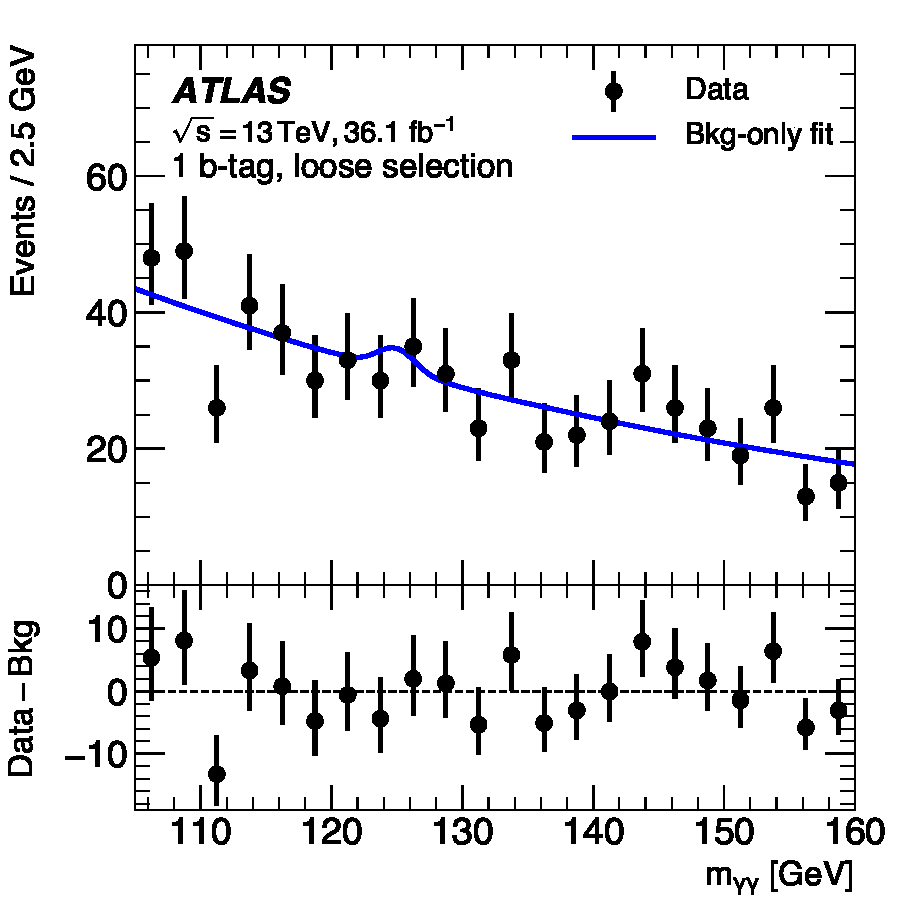
\includegraphics[width=0.48\textwidth]{chapters/chapter5_yybb/images/results/m_yy_lowMass_1tag_bkg_fit_to_data_withRatio}}
	\quad
	\subfloat[]{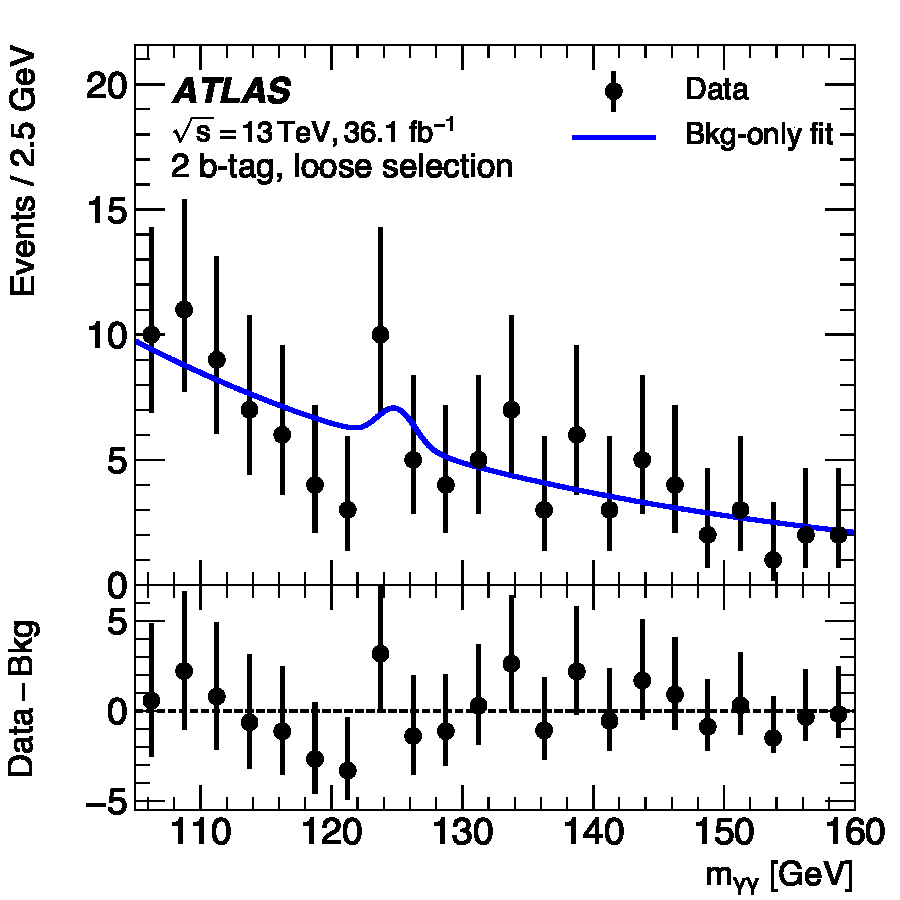
\includegraphics[width=0.48\textwidth]{chapters/chapter5_yybb/images/results/m_yy_lowMass_2tag_bkg_fit_to_data_withRatio}}
	\\
	\subfloat[]{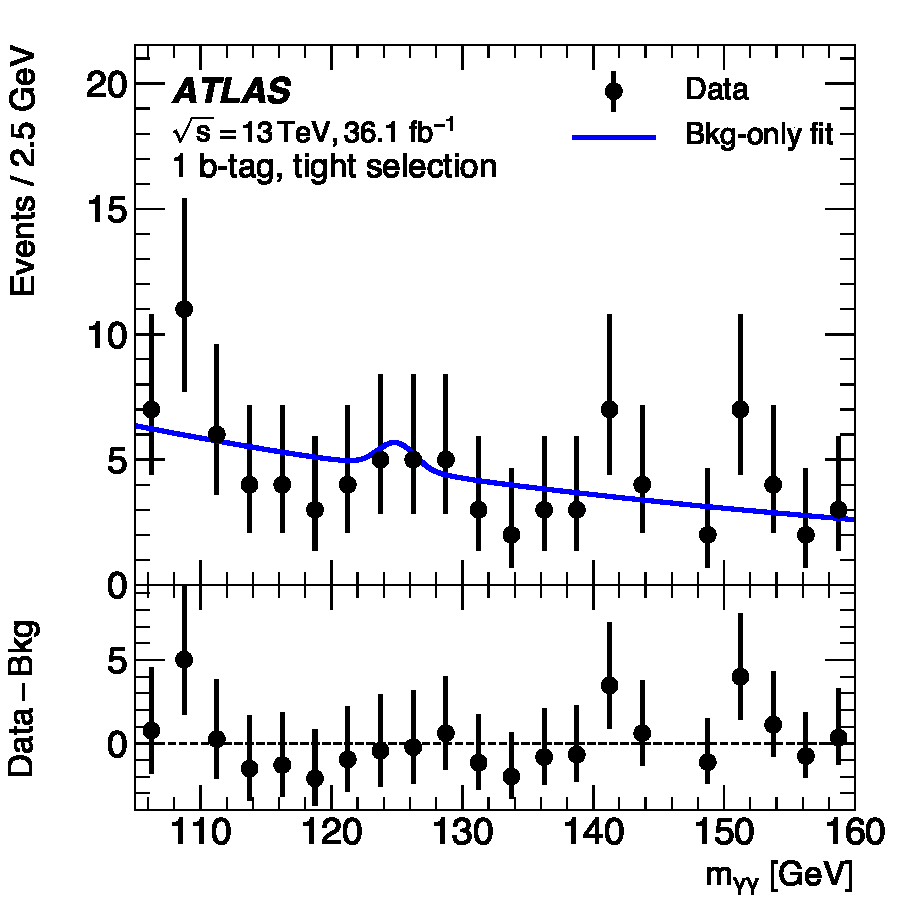
\includegraphics[width=0.48\textwidth]{chapters/chapter5_yybb/images/results/m_yy_highMass_1tag_bkg_fit_to_data_withRatio}}
	\quad
	\subfloat[]{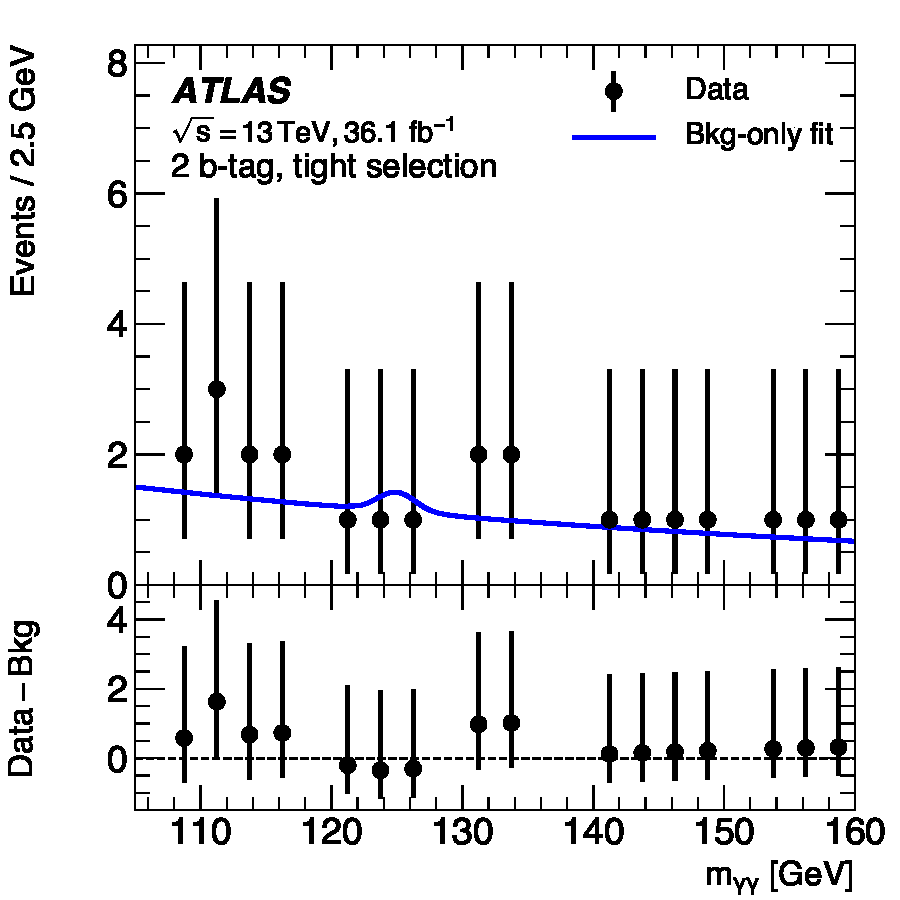
\includegraphics[width=0.48\textwidth]{chapters/chapter5_yybb/images/results/m_yy_highMass_2tag_bkg_fit_to_data_withRatio}}
	\caption{Data and background-only fits for each of the analysis categories in the non-resonant analysis. The background fit is composed of the smoothly-falling continuum \yy background as well as the single Higgs boson production background, peaking around $\unit{125}{\GeV}$.}
  \label{fig:results-myy}
\end{figure}


\begin{figure}[htbp]
  \centering
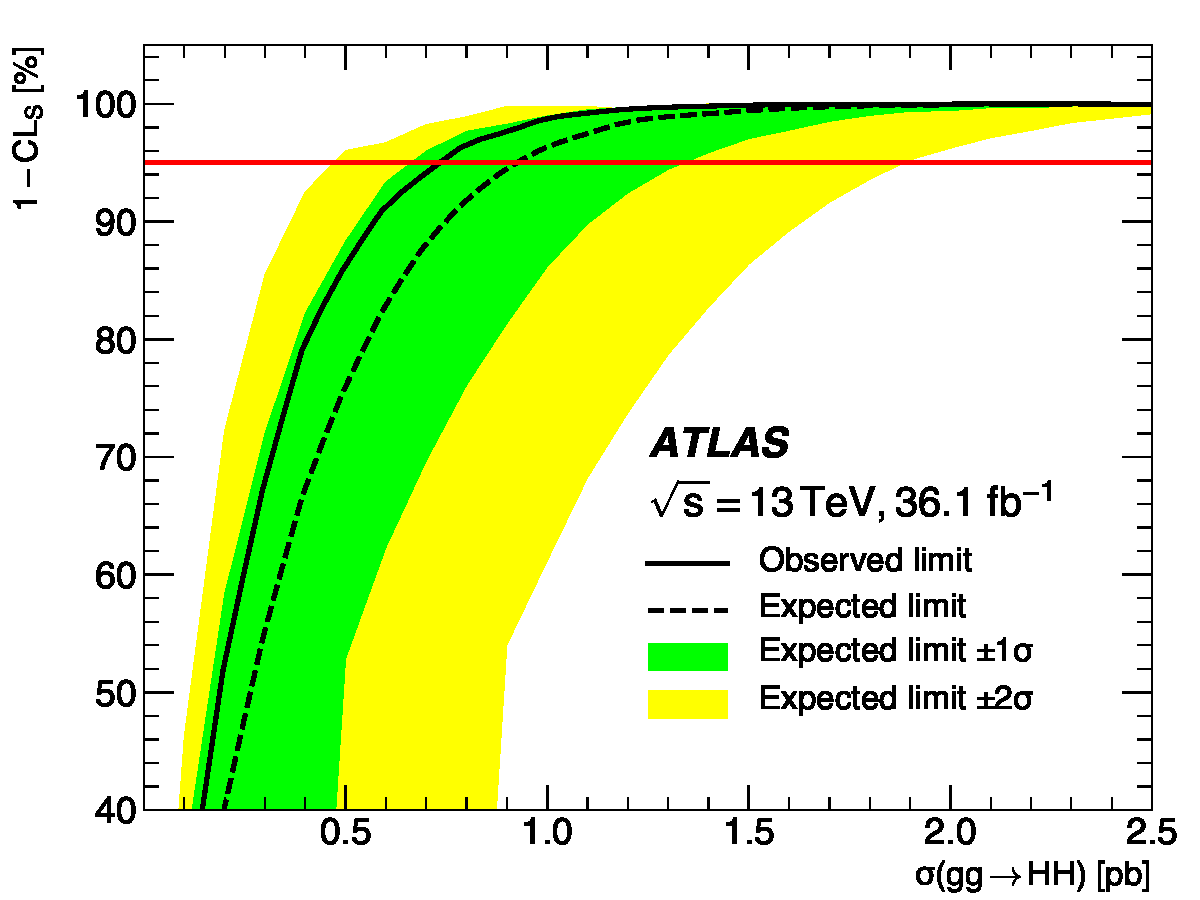
\includegraphics[width=0.9\textwidth]{chapters/chapter5_yybb/images/limits/nonresonant.pdf}
  \caption[The expected and observed limits on the non-resonant HH production cross section]
  {The expected and observed 95\% \gls{CL} limits on the non-resonant HH production cross section, $\sigma_{gg\rightarrow HH}$. These limits are set using the tight analysis selection. The 95\% confidence level is indicated by the red horizontal line.}
  \label{fig:limits-nonresonant}
\end{figure}

\subsection{Limits on Resonant Production}

The 95\% \gls{CL} limits on resonant di-Higgs production are shown in Figure \ref{fig:limits-resonant}. This limit uses the loose selection at $m_{X} \leq \unit{500}{\GeV}$ and the tight selection at $m_{X} \geq \unit{500}{\GeV}$. No significance excesses are found. Expected exclusion limits range from 1.14 pb to 0.12 pb, observed limits range from 0.90 pb to 0.15 pb.

\begin{figure}[htbp]
  \centering
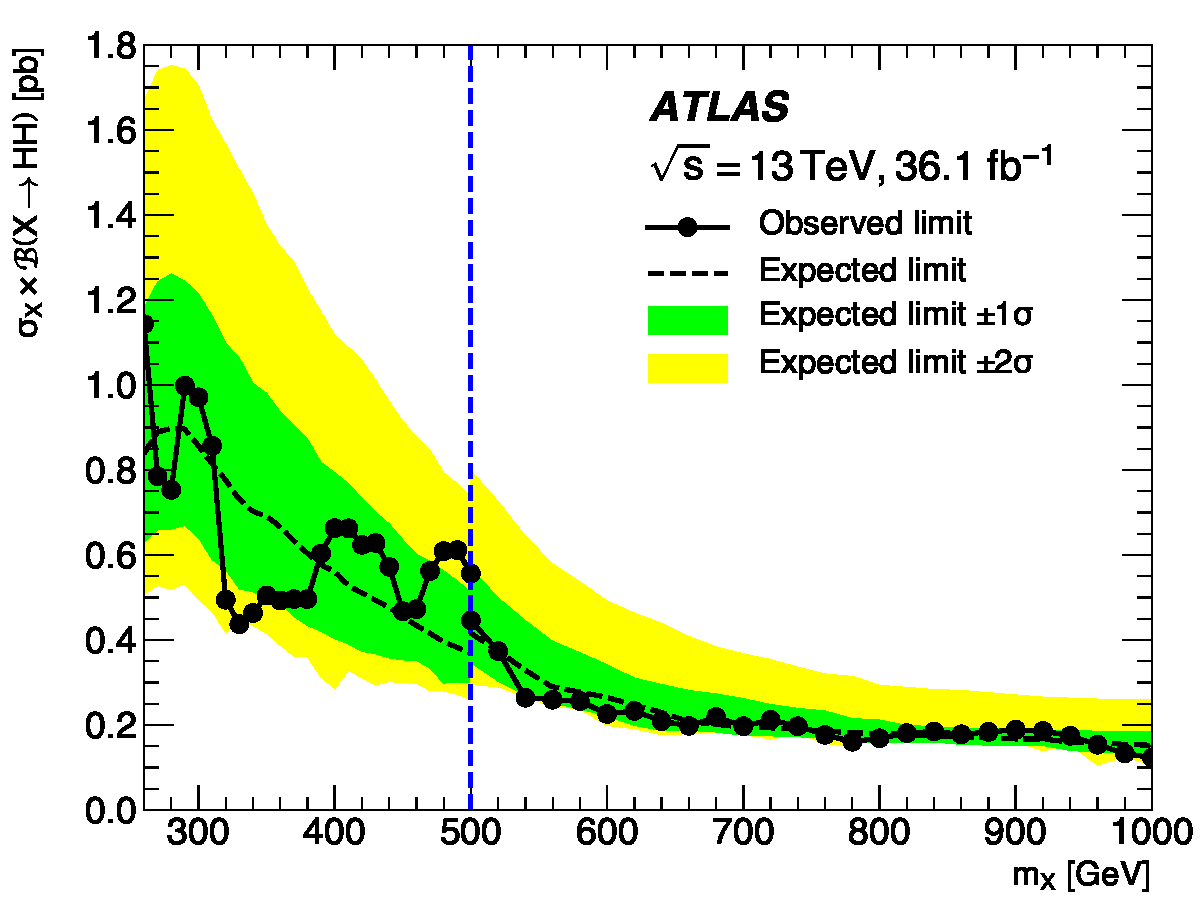
\includegraphics[width=0.9\textwidth]{chapters/chapter5_yybb/images/limits/resonant.pdf}
\caption[The expected and observed limits on the resonant \HH production cross section as a function of $m_{X}$.]
{The expected and observed 95\% \gls{CL} limits on the resonant \HH production cross-section, $\sigma_{X} \times \mathcal{B}(X\rightarrow HH)$, as a function of $m_{X}$. The loose selection is used in the low mass regime, $m_{X} \leq \unit{500}{\GeV}$, while the tight selection is used in the high mass regime, $m_{X} \geq \unit{500}{\GeV}$. The transition point between these selections is indicated by the dashed line.} 
\label{fig:limits-resonant}
\end{figure}

\subsection{Limits on the Trilinear Higgs Coupling}

Limits are set on \klambda using the asymptotic formula. The exclusion as a function of \klambda is shown in figure , corresponding to $-8.2 < \klambda < 13.3$.

\begin{figure}[htbp]
  \centering
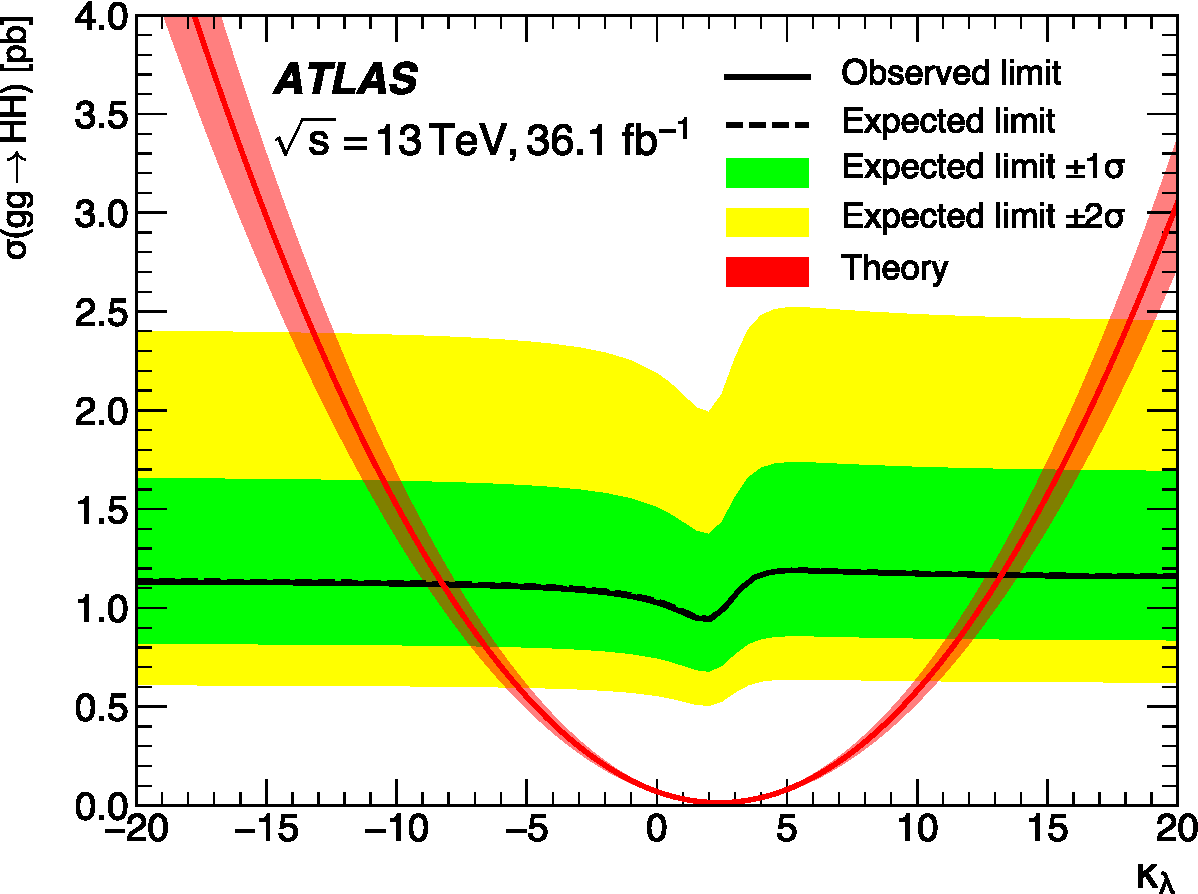
\includegraphics[width=0.9\textwidth]{chapters/chapter5_yybb/images/limits/lambda.pdf}
\caption[The expected and observed limits on the non-resonant \HH production cross section as a function of \klambda]
{The expected and observed 95\% \gls{CL} limits on the non-resonant \HH production cross section as a function of \klambda. The red line indicated the predicted $HH$ cross-section for varied \klambda, assuming all other couplings are equivalent to \gls{SM} prediction, the band includes theoretical uncertainty.} 
\label{fig:limits-klambda}
\end{figure}

\section{Searches for Vector Boson Fusion HH Production}

To improve this analysis, a signal model for the Vector Boson Fusion production mode has been designed and will be implemented into this analysis using the full ``Run 2'' dataset. This signal model is integrated into the analysis through a separate analysis category that is enriched in VBF events, defined via cuts on multiclass \gls{BDT} scores.

\subsection{Simulated Samples}

\subsubsection{Non-resonant VBF HH Samples}

The signal MC samples for VBF $HH$ production are generated at LO using \MGMCatNLO 2.6.0, using cards presented in \cite{vbfhh}. The process generated is $pp \rightarrow HHqq$. The dominant production in this sample is VBF $HH$ production, but contains contributions from $VHH$  hadronic and Higgsstrahlung production. The NNPDF 2.3 LO PDF set \cite{NNPDF} is used in the matrix element, interfaced to \HERWIG 7.0.4 using the H7-UE-MMHT tune for underlying events and the H7-MMHT2014LO tune for parton shower and hadronization.

Samples have been produced for the various coupling values shown in Table \ref{tab:vbf-coupling-samples}. The values of $\kappa_\lambda$,$c_{2V}$, and $c_{v}$ are all 1 in the SM. The values selected for production aim to vary each coupling value enough that interpolation may be performed, and one value was produced near where limits could be expected to be set ($\kappa_\lambda = 10$ and $c_{2V}=4$).

\begin{table}[htbp]
    \centering
    \caption{Grid of coupling values used in production of VBF $HH$ samples.}
    \begin{tabular}{c|c|c}
        $\kappa_\lambda$ & $c_{2V}$ & $c_{v}$ \\
        \hline
        1 & 0 & 0.5 \\
        1 & 1 & 0.5 \\
        0 & 0 & 1 \\
        1 & 0 & 1 \\
        1 & 0.5 & 1 \\
        1 & 0 & 0.5 \\
        1 & 1 & 1 \\
        1 & 1.5 & 1 \\
        1 & 2 & 1 \\
        1 & 4 & 1 \\
        0 & 1 & 1 \\
        2 & 1 & 1 \\
        10 & 1 & 1 \\
        1 & 1 & 1.5
    \end{tabular}
    \label{tab:vbf-coupling-samples}
\end{table}

Relevant distributions for validation of these samples can be seen in Figure \ref{fig:vbf-mc-validation}. Plots are shown at parton level, with a basic jet selection applied to isolate the VBF jets similar to that done at reconstruction level. Jets are considered if they have $\pt > 25$, then the $m_{bb}$ pair is selected as the two jets with $m_{bb}$ closest to 125 \GeV. The VBF jets are selected as the highest $m_{jj}$ pair after removing jets used in the $m_{bb}$ pairing. Additional detail on the validation for these samples is outlined in Ref. \cite{mc-validation}.

\begin{figure}[htbp]
    \centering
    \subfloat{
      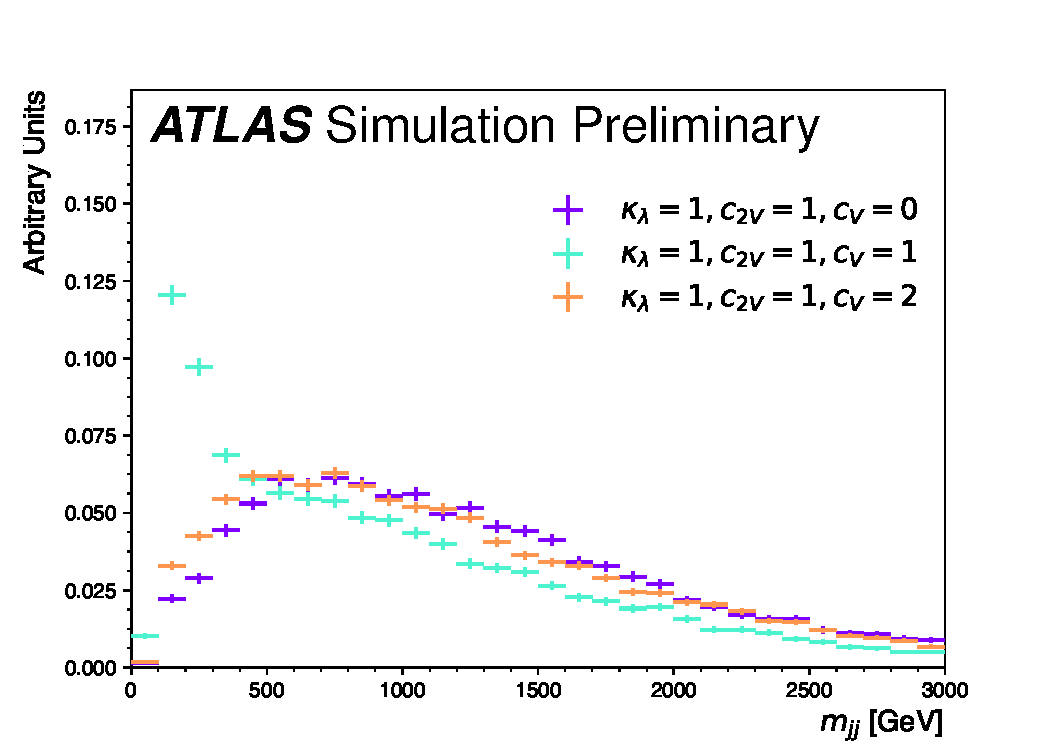
\includegraphics[width=0.33\textwidth]{chapters/chapter5_yybb/images/mc_samples/m_jj_cv.pdf}
    }
    \subfloat{
      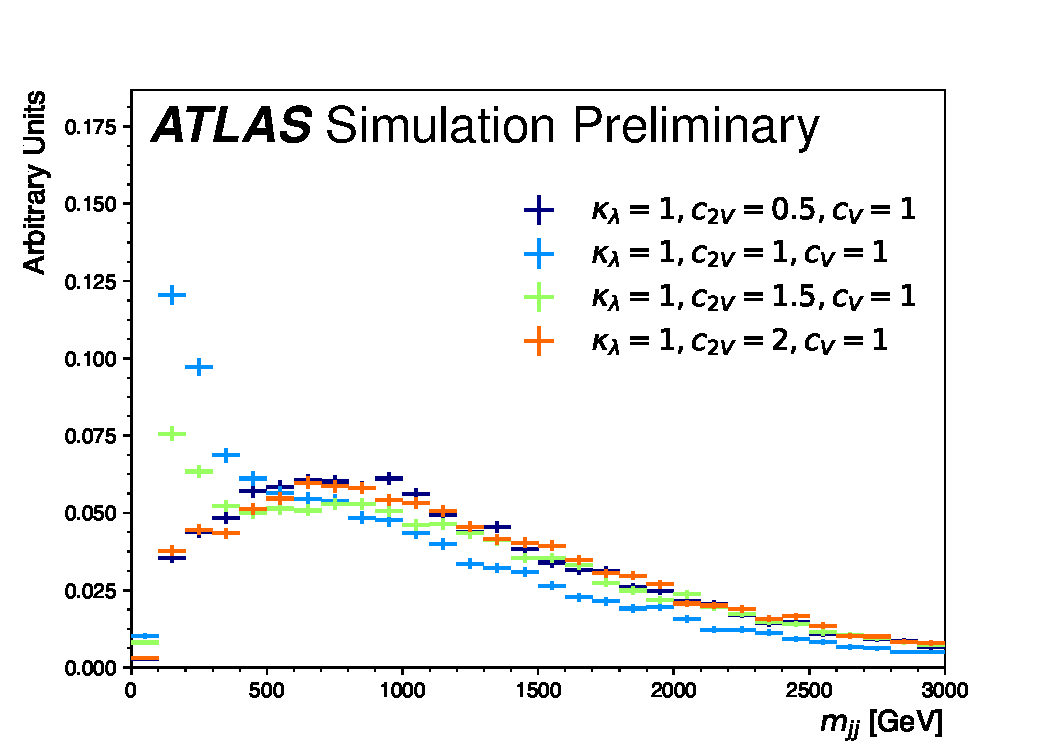
\includegraphics[width= 0.33\textwidth]{chapters/chapter5_yybb/images/mc_samples/m_jj_cvv.pdf}
    }
    \subfloat{
      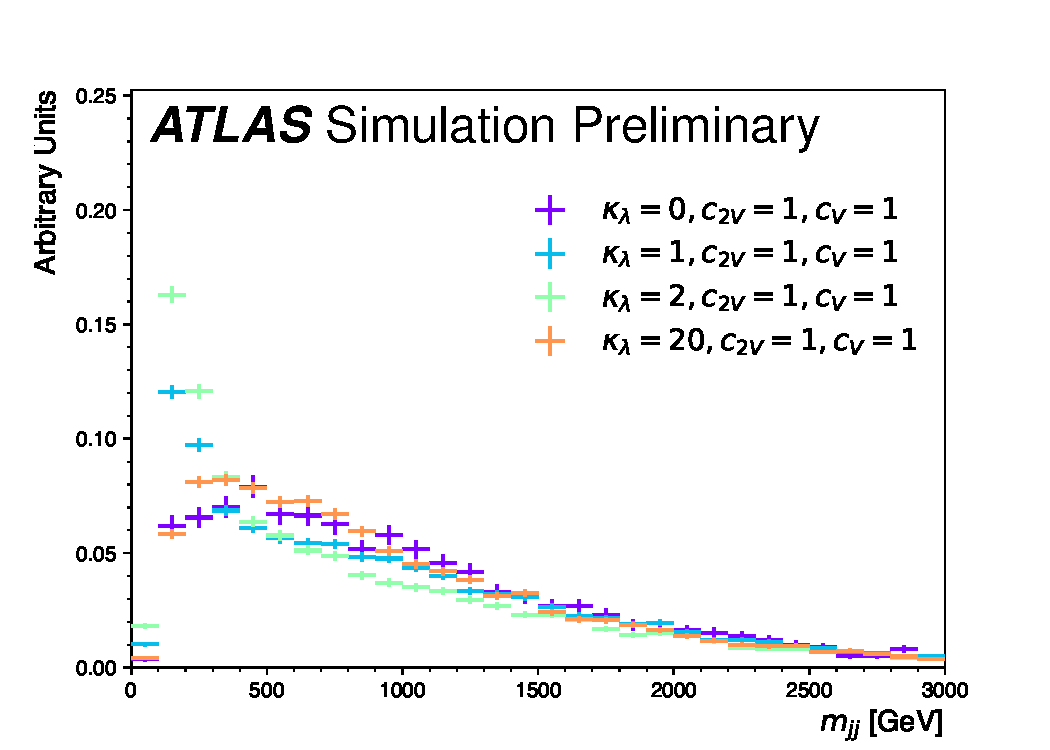
\includegraphics[width= 0.33\textwidth]{chapters/chapter5_yybb/images/mc_samples/m_jj_klambda.pdf}

    }       

    \subfloat{
        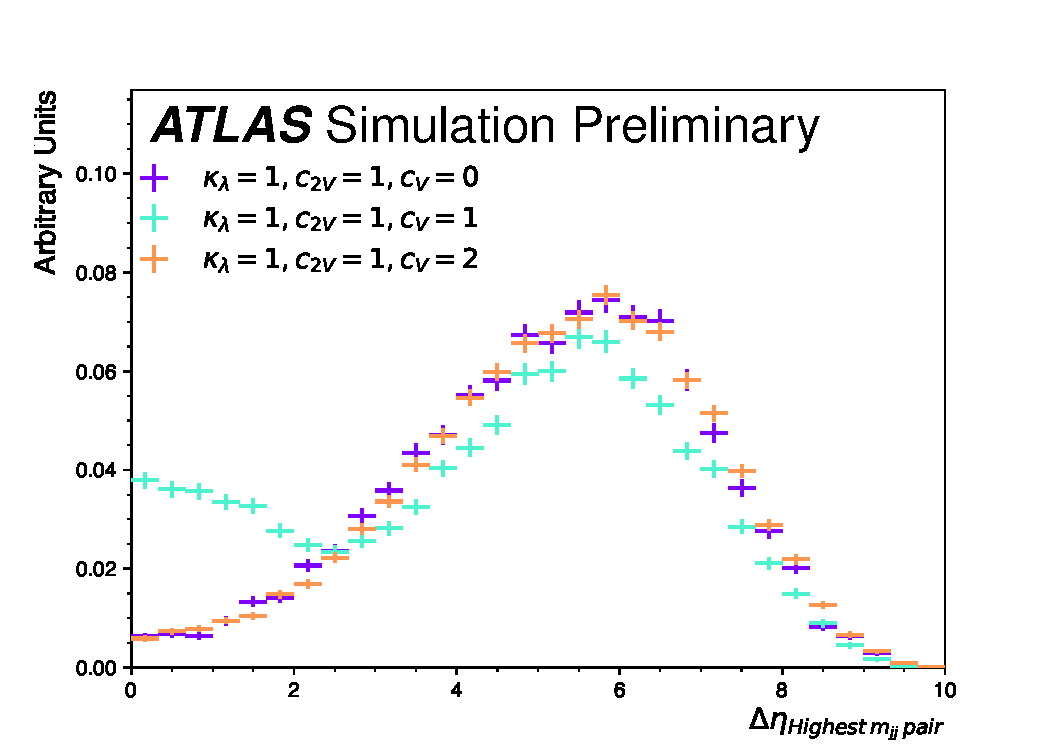
\includegraphics[width=0.33\textwidth]{chapters/chapter5_yybb/images/mc_samples/jj_deta_cv.pdf}
      }
      \subfloat{
        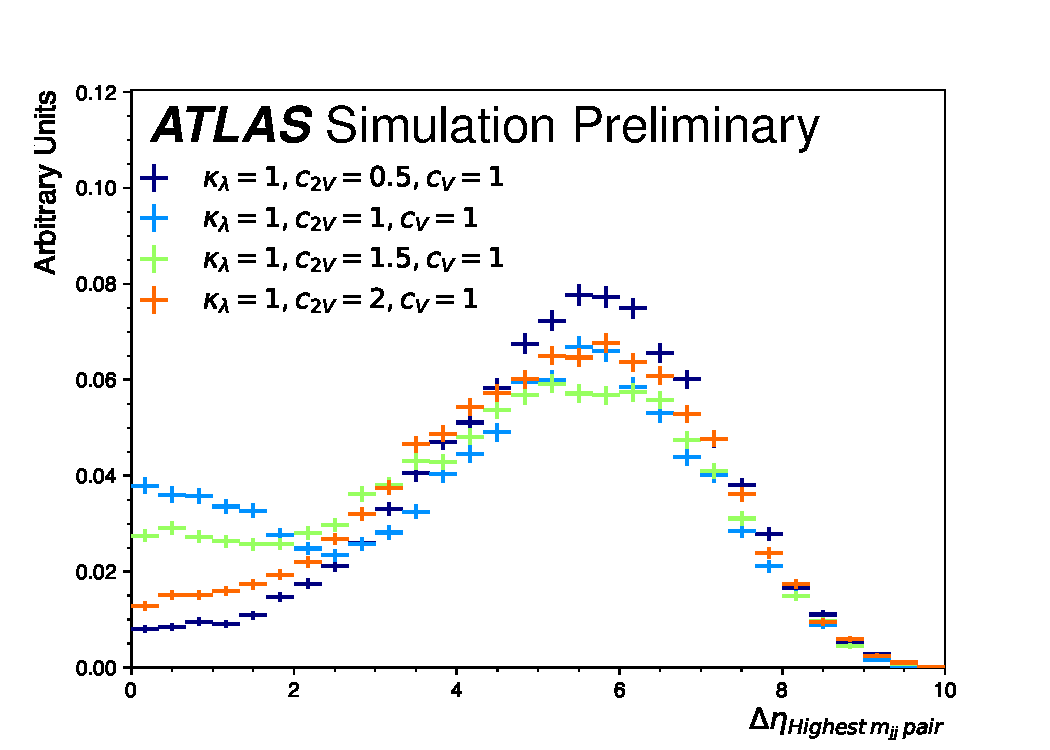
\includegraphics[width= 0.33\textwidth]{chapters/chapter5_yybb/images/mc_samples/jj_deta_cvv.pdf}
      }
      \subfloat{
        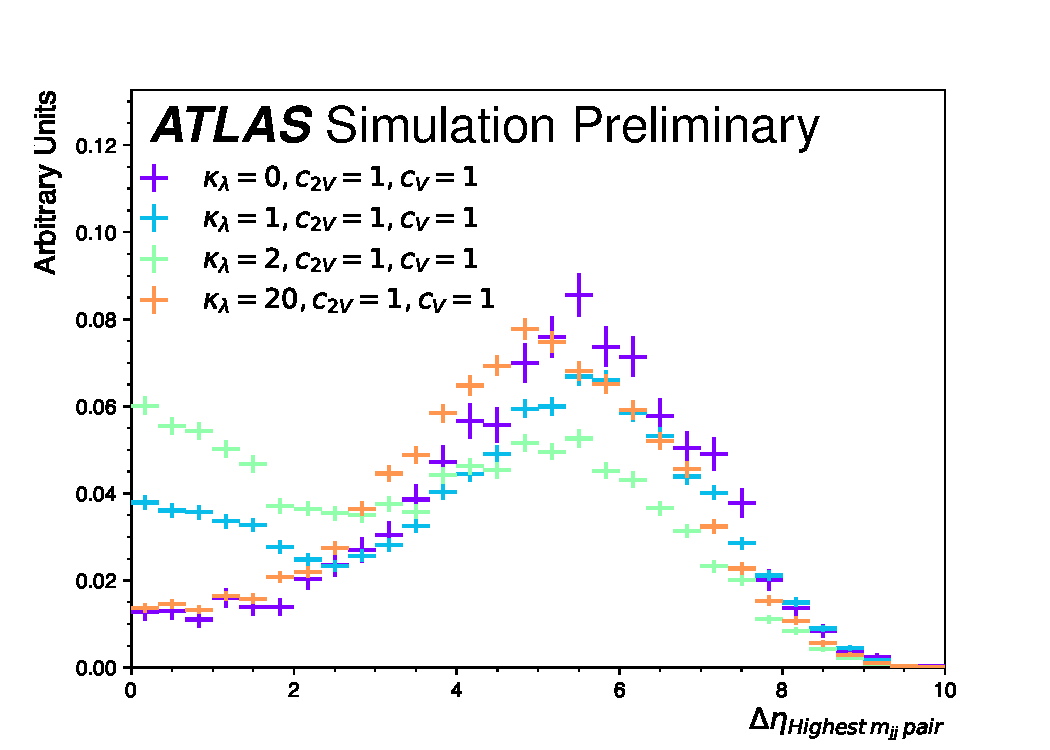
\includegraphics[width= 0.33\textwidth]{chapters/chapter5_yybb/images/mc_samples/jj_deta_klambda.pdf}
    }    

    \caption{Validation plots at parton level for the VBF $HH$ signal sample. The highest $m_{jj}$ pair is selected as a proxy for the VBF jets. The top row shows the invariant mass distribution of this system, the bottom depicts the $\Delta \eta$ between these jets. Left to right, these plots vary the $c_V$, $c_{2V}$, and $\kappa_\lambda$ strength. The peak at low $m_{jj}$ values and shoulder at low $\Delta \eta$ is a product of the $VHH$ hadronic and Higgsstrahlung contributions in the samples.}
    \label{fig:vbf-mc-validation}
\end{figure}

\subsection{Event Selection} \label{ssec:vbf-event-selection}
Events which have already passed the ggF BDT based selection and have at least 4 jets are considered for the VBF candidate. The 4 jet requirement is imposed in order to reconstruct VBF-based variables. The VBF jets are then selected as the highest $m_{jj}$ pairing, excluding $H\rightarrow b\bar{b}$ candidate jets.

These events are then evaluated by a multiclass BDT, which has independent classes for VBF HH, ggF HH, $\gamma \gamma$-continuum, and $ttH$. Ultimately, an event selected for the VBF category if it passes the BDT score threshold for VBF HH, and fails the score threshold for the other three classes. The thresholds are determined by a 4-dimensional scan over cuts on the BDT score, with the Asimov significance as the figure of merit.

A flowchart of this logic is shown in Figure \ref{fig:vbf-logic}.

\begin{figure}[htbp]
    \centering
	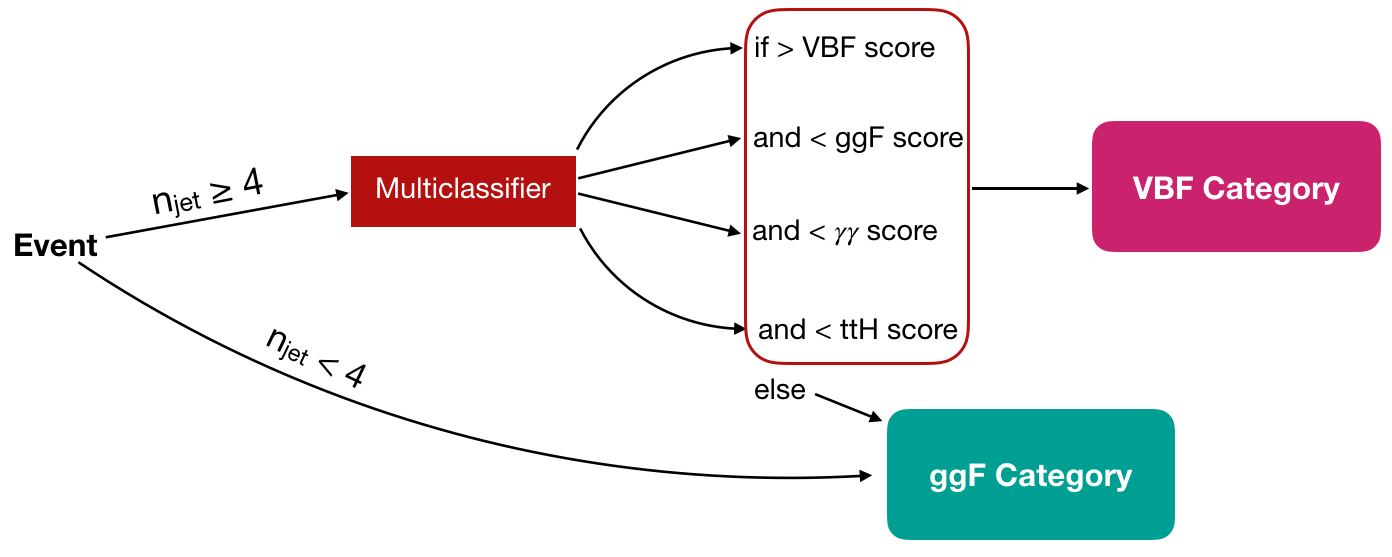
\includegraphics[width=0.9\textwidth]{chapters/chapter5_yybb/images/vbf_logic.png}
    \caption{Logic flow for an event to be selected into the VBF-enriched signal region. The starting set of candidates (denoted ``event'') requires passing preselection and at least one of the ggF-based signal categories. If an event is assigned to the ggF categories, it is separated into 4 categories.}
    \label{fig:vbf-logic}
\end{figure}


\begin{center}
	\begin{tabular}{c|c|c}
	\hline
	Class & Target & Selection Logic  \\
	\hline
	0 & VBF HH & $BDTscore_{0} > XXX $ \\
	1 & ggF HH & $BDTscore_{1} < XXX $ \\
	2 & $\gamma\gamma$-Continuum &  $BDTscore_{2} < XXX $ \\
	3 & $ttH$ &  $BDTscore_{3} < XXX $ \\
	\hline
	\end{tabular}
\end{center}


A set of 26 variables were considered for this BDT, listed in Appendix \ref{app:vbf-variables}. Broadly, they describe the kinematics of various physics objects in the event, as well as event shape \cite{STDM-2011-33} variables and variables to reconstruct the W-mass, which are useful for suppression of the ttH background.

For dimensionality reduction, a pruning procedure was performed.
\begin{enumerate}
  \item To remove redundant variables, those with a pearson correlation value above 0.85 were removed. This brought the list from 26 to 19, pruning several event shape variables.
  \item After pruning those variables and retraining, low-impact variables were removed. The pearson correlation for each variable to the 4 class BDT probability distributions were calculated. Those 4 correlation values were summed, and variables with a sum less than 1.0 were pruned. This brought the set from 19 to 11 input variables.
  \item At 11 input variables, the number of possible combinations of variables has vastly simplified, so every possible variable subset was considered, with a depth optimization procedure performed with each retraining. The minimal subset of variables which did not impact the final significance was selected as the final inputs.
\end{enumerate}

After this pruning procedure, the X final inputs were:

\textbf{VBF-targeted:}

\textbf{$\gamma \gamma$-suppressing:}

\textbf{$ttH$-suppressing:}



Distributions for each these variables after applying a 4-jet requirement can be found in Appendix \ref{app:vbf-variables}.

Adding a VBF-enriched category provides a XXX percent improvement over not defining such a category.


\subsection{Analysis Improvement}

